\documentclass[a4paper,twoside,11pt]{article}
\usepackage[a4paper,left=2cm,right=2cm,top=2cm,bottom=2cm]{geometry}
\usepackage{fancyhdr}
\pagestyle{fancy}
\fancyhf{}
\chead{ECON 469 Review Notes}
\lhead{Winter 2021}
\rhead{Caiwei Xiong}
\cfoot{\thepage}
\usepackage[utf8]{inputenc}
\usepackage[T1]{fontenc}
\usepackage{lmodern}
\usepackage{graphicx}
\usepackage[figurename=Fig.,labelfont=bf,labelsep=period]{caption}
\usepackage{subcaption}
\usepackage{amsmath}
%\usepackage{amsfonts}
%\usepackage{amssymb}
%\usepackage{amsbsy}
\usepackage{newtxtext,newtxmath}
\usepackage[dvipsnames]{xcolor}
\usepackage{amssymb}
\usepackage{graphicx}
\usepackage{listings}
\usepackage{framed} 
\usepackage[english]{babel}
\definecolor{shadecolor}{rgb}{0.94,0.97,1.0} \definecolor{c1}{HTML}{FFFFCC}

\begin{document}
\begin{shaded*}
\section{White Noise}
\noindent If $\mu=0$, and $\gamma_k =0$ for all $k \ne 0$, we say that $\{y_t\}$ is a \textbf{white noise process}
\newline
\newline
If it is independent over time, then we say it is an independent white noise.
\end{shaded*}
\section{Static time series regression models}
\noindent A static model models the contemporaneous relationship between two(or more) variables. 
\begin{equation*}
\begin{aligned}
    y_t = \beta_1 + \beta_2 x_t + e_t
\end{aligned}
\end{equation*}
where $(y_t,x_t)$ are both observed at time $t$. 
\newline
\textcolor{NavyBlue}{\textbf{Static models are not good for forecasting}}
\begin{itemize}
    \item they ignore the fact that usually past outcomes on $y$ help predict further values of $y$
    \item to forecast $y_{t+1}$ at time $t$ \textcolor{NavyBlue}{we would have to know or forecast $x_{t+1}$ at time $t$}
\end{itemize}
\section{Finite distributed lag models}
\noindent Static models do not capture effects that take place with a lag
\newline
\textcolor{NavyBlue}{If we think that a variable $x$ affects $y$ up to a finite number of periods into the future} $\rightarrow$ FDL model is appropriate
\begin{equation*}
\begin{aligned}
    y_t = \beta_1 + \delta_0 x_t + \delta_1 x_{t-1} + \delta_2 x_{t-2} + e_t
\end{aligned}
\end{equation*}
\textbf{\textcolor{NavyBlue}{Interpret $\delta_0,\delta_2$ and $\delta_2$}}
\noindent Suppose that $x_t=0$ for all $t<0$. At time $t=0,  x_0 =1$, and it reverts to $0$ after that. ($e_t=0$)
\begin{center}
\begin{tabular}{ c c c c c c c c } 
 \hline
 $t$ & $\cdots$ & -1 & 0 & 1 & 2 & 3 & $\cdots$ \\
 $x_t$ & $\cdots$ & 0 & 1 & 0 & 0 & 0 & $\cdots$ \\ 
 $y_t$ & $\cdots$ & $\beta_1$ & $\beta_1 + \delta_0$ & $\beta_1 + \delta_1$ & $\beta_1 + \delta_2$ & $\beta_1$ & $\cdots$ \\
 $y_t - y_{-1}$ & $\cdots$ & 0 & $\delta_0$ & $\delta_1$ & $\delta_2$ & 0 & $\cdots$\\
 \hline
\end{tabular}
\end{center}
\textcolor{NavyBlue}{$\delta_0$} is called the impact multiplier. ( it gives the immediate change in $y$ due to a temporary one-unit increase on $x$)
\newline
\textcolor{NavyBlue}{$\delta_1$ and $\delta_2$} are dynamic multipliers($\delta_1$ gives the change in $y$ one period after the change in $x$, $\delta_2$ gives the change in $y$ two periods after the change in $x$. 
\subsection{Long run multiplier/propensity}
\begin{equation*}
\begin{aligned}
    y_t = \beta_1 + \delta_0 x_t + \delta_1 x_{t-1} + \delta_2 x_{t-2} + e_t
\end{aligned}
\end{equation*}
\textbf{\textcolor{NavyBlue}{Interpret $\delta_0,\delta_2$ and $\delta_2$}}
\noindent Suppose that $x_t=0$ for all $t<0$. At time $t=0,  x_0 =1$, and it reverts to $0$ after that. ($e_t=0$)
\begin{center}
\begin{tabular}{ c c c c c c  } 
 \hline
 $t$ &  -1 & 0 & 1 & 2 & 3  \\
 $x_t$  & 0 & 1 & 1 & 1 & 1  \\ 
 $y_t$ & $\beta_1$ & $\beta_1 + \delta_0$ & $\beta_1 +\delta_0+ \delta_1$ & $\beta_1 +\delta_0+ \delta_1 + \delta_2$ & $\beta_1+\delta_0+ \delta_1 + \delta_2$  \\
 $\bigtriangleup y$  & 0 & $\delta_0$ & $\delta_0+ \delta_1$ & $\delta_0+ \delta_1+\delta_2$ & $\delta_0+ \delta_1+\delta_2$\\
 \hline
\end{tabular}
\end{center}
\textcolor{NavyBlue}{$\delta_0+\delta_1$} gives $\bigtriangleup y$ one period after the permanent $\bigtriangleup x$ 
\newline
\textcolor{NavyBlue}{$\delta_0 + \delta_1 + \delta_2$} gives $\bigtriangleup y$ two periods after the permanent $\bigtriangleup x$
\newline
$\rightarrow$ for a FDL model of order $2$, the long run multiplier/propensity:
\begin{equation*}
\begin{aligned}
    LRP = \delta_0 + \delta_1 + \delta_2
\end{aligned}
\end{equation*}
$95\%$ confidence interval for LRM:
\begin{equation*}
\begin{aligned}
    \hat \theta_0 \pm 1.96 \times se(\hat \theta_0)
\end{aligned}
\end{equation*}
\begin{itemize}
    \item the OLS estimators are no longer unbiased under any assumptions
    \item large sample analysis is also very important for static and FDL models
    \item large-sample analysis is much trickier with time series data because of correlation across time. With cross-sectional data, we can rely on random sampling
\end{itemize}
\subsection{Finite sample properties of OLS} 
\noindent Consider the time series regression model
\begin{equation*}
\begin{aligned}
    y_t = x_t' \beta + e_t \ \ \ \ t=1,\cdots, T
\end{aligned}
\end{equation*}
This notation accommodates static, FDL and lagged dependent variable model
\newline
\textcolor{NavyBlue}{If the Gauss-Markov assumptions hold, OLS is BLUE.}
\begin{shaded*}
\noindent \textbf{Gauss-Markov assumptions:}
\begin{equation*}
\begin{aligned}
        rank (X) =& k \\
        E(e|X) =& 0 \\
        Var(e|X) =& \sigma^2 I_T \\
\end{aligned}
\end{equation*}
\end{shaded*}
\subsection{Strict exogeneity for time series regressions}
Suppose:
\begin{equation*}
\begin{aligned}
y_t = x_t'\beta + e_t \ \ \ \ t=1,\cdots, T
\end{aligned}
\end{equation*}
Strict exogeneity assumption:
\begin{equation*}
\begin{aligned}
    E(e_t|X)=0 \ \ \forall \ t
\end{aligned}
\end{equation*}
\textcolor{NavyBlue}{A very strong assumption: 
\begin{itemize}
    \item feedback effects from $y$ into $x$
    \item lagged dependent variables as regressors
\end{itemize}}
\subsection{Strict exogeneity in FDL models} 
Suppose: 
\begin{equation*}
\begin{aligned}
    y_t = \beta_1 + \delta_0 x_t + \delta_1 x_{t-1} + \delta_2 x_{t-2} + e_t
\end{aligned}
\end{equation*}
\textcolor{NavyBlue}{$e_t$ to be uncorrelated with all past and future values of $x$}
\subsection{Assumption on the variance-covariance matrix}
\noindent $\because Var(e|X)=\sigma^2 \cdot I_T$ 
\newline
$\therefore Var(e_t |X)=\sigma^2 \ \ \  \forall \ t \ \ \ \ and \ \ \ \ \  Cov(e_t,e_s|X)=0 \ \ \ \ \forall t \ne s$
\newline
\newline
\textcolor{NavyBlue}{$Var(e_t |X)=\sigma^2 \ \ \  \forall \ t$} is the assumption of homoskedasticity(both conditional and unconditional)
\begin{itemize}
    \item $Var(e_t|X)=Var(e_t)=]sigma^2$
    \item variance of $e_t$ does not depend on $X$ and is constant over time. 
\end{itemize}
\textcolor{NavyBlue}{$Cov(e_t,e_s|X)=0 \ \ \ \ \forall t \ne s$} is the assumption of no serial correlation
\begin{itemize}
    \item regression errors need to be \textcolor{NavyBlue}{white noise}
    \item this assumption does not prevent $y_t$ or $x_t$ to be serially correlated
\end{itemize}
\section{Covariance-Stationarity}
\noindent \textcolor{NavyBlue}{$\gamma_k$ is the autocovariance function}
\newline
The stochastic process $\{y_t \}$ is covariance stationary (\textcolor{NavyBlue}{weakly stationary}) if:
\begin{equation*}
\begin{aligned}
   E(y_t) = \mu
\end{aligned}
\end{equation*}
is independent of $t$, and 
\begin{equation*}
\begin{aligned}
\gamma_{k,t} \equiv Cov(y_t, y_{t-k}) = E[(y_t -\mu)(y_{t-k}-\mu)]=\gamma_k
\end{aligned}
\end{equation*}
is independent of $t$ for all $k$
\newline
\textcolor{NavyBlue}{The autocorrelation function is:}
\begin{equation*}
\begin{aligned}
  \rho_k = \frac{\gamma_k}{\gamma_0}
\end{aligned}
\end{equation*}
\subsection{Strict Stationarity}
\noindent $\{y_t\}$ is strictly stationary if the joint distribution of $(y_t, y_{t-1},\cdots, y_{t-k})$ does not depend on $t$ for all $k$. (The marginal distributions of $y_t$ are also invariant over time)
\newline
$\{y_t\}$ is strictly stationary $\Rightarrow \{y_t\}$ is covariance stationary
\begin{itemize}
    \item the opposite is not true
    \item the only exception is if the process is Gaussian (under Gaussianity, the joint distribution is completely characterized by the mean and covariance matrix).
\end{itemize}
\subsection{Stationarity and LLN}
\subsubsection{Weak dependence}
\noindent $\{y_t\}$ is "weakly dependent" if $y_t$ and $y_{t-k}$ become approximately independent as $k$, the distance between them, increases.
\newline
$\Rightarrow$ we will require $\{y_t\}$ to become "asymptotically uncorrelated"
\begin{equation*}
\begin{aligned}
\gamma_k \rightarrow 0 \ \ as \ \ k \rightarrow \infty
\end{aligned}
\end{equation*}
\textcolor{NavyBlue}{For LLN's and CLT's to apply, we need $\gamma_k \rightarrow 0$ sufficiently fast so that}
\begin{equation*}
\begin{aligned}
\sum^\infty_{k=0} |\gamma_k| < \infty
\end{aligned}
\end{equation*}
\textcolor{NavyBlue}{Under stationarity and weak dependence, we can show that}
\begin{equation*}
\begin{aligned}
\hat \gamma_k \equiv \frac{1}{T} \sum^T_{t=1+k}(y_t - \bar y)(y_{t-k} - \bar y) \overset{P}{\rightarrow} \gamma_k = Cov(y_t, y_{t-k})
\end{aligned}
\end{equation*}
a result that also holds for i.i.d. data.
\section{Moving average processes of order larger than 1}
\subsection{Lag operators}
\noindent The lag operator is defined as $L_{x_t}=x_t-1$
\newline
$L$ is a distributive and associative operator.(we can define a polynomial of degree $m$ in $L$ as):
\begin{equation*}
\begin{aligned}
\phi(L) = 1+ \phi_1 L + \cdots + \phi_m L^m
\end{aligned}
\end{equation*}
implying that
\begin{equation*}
\begin{aligned}
\phi(L)_{x_t} = x_t + \phi_1 x_{t-1} + \cdots + \phi_m x_{t-m}
\end{aligned}
\end{equation*}
If $|\phi_1| <1$ 
\begin{equation*}
\begin{aligned}
(1- \phi_1 L)^{-1} = 1+ \phi_1 L + \phi_1^2 L^2 + \cdots = \sum^\infty_{j=0} \phi_1^j L^j
\end{aligned}
\end{equation*}
ARMA Processes: let $\phi(L)$ as above and let 
\begin{equation*}
\begin{aligned}
\theta(L)=1+\theta_1 L + \theta_2 L^2 + \cdots + \phi_q L^q 
\end{aligned}
\end{equation*}
Then:
\begin{equation*}
\begin{aligned}
\phi(L)y_t =& \theta(L) \epsilon_t \\
\Leftrightarrow \\
y_t =& \phi_1 y_{t-1} + \cdots + \phi_p y_{t-p} + \epsilon_t +\theta_1 \epsilon_{t-1}+\cdots +\theta_q \epsilon_{t-q}
\end{aligned}
\end{equation*}
\begin{shaded*}
\noindent AR processes: let
\begin{equation*}
\begin{aligned}
\phi(L) = 1- \phi_1L - \phi_2 L^2 -  \phi_p L^p
\end{aligned}
\end{equation*}
Then: 
\begin{equation*}
\begin{aligned}
\phi(L)y_t = \epsilon_t
\end{aligned}
\end{equation*}
is equivalent to
\begin{equation*}
\begin{aligned}
y_t = \phi_1 y_{t-1} + \cdots + \phi_p y_{t-p} + \epsilon \sim AR(p)
\end{aligned}
\end{equation*}

\subsection{AR(1) Process}
\noindent $y_t \sim AR(1)$ if
\begin{equation*}
\begin{aligned}
y_t = c + \phi_1 y_{t-1} + \epsilon_t
\end{aligned}
\end{equation*}
where $\epsilon_t$ is white noise.
\newline
This is equivalent to 
\begin{equation*}
\begin{aligned}
(1- \phi_1 L)y_t = c+ \epsilon_t
\end{aligned}
\end{equation*}
where $\phi(L)$ denotes a polynomial of degree one in $L$. 
\newline
\textcolor{NavyBlue}{The crucial condition is that $|\phi|<1$}
\subsection{Mean and variance of a stationary AR(1) process}
\begin{equation*}
\begin{aligned}
E(y_t) =& \ \frac{c}{1-\phi_1} \equiv \mu \\
\gamma_0 =& \  Var(y_t) = \frac{\sigma^2}{ 1-\phi_1^2} \\
\gamma_1 =& \  Cov(y_t, y_{t-1}) = \phi_1 \gamma_0 \\
\gamma_k =& \ \phi_1^k \frac{\sigma^2}{1- \phi_1^2} \ \ \ \ \textmd{for} \ k=0,1,2,\cdots \\
\rho_k =& \ \frac{\gamma_k}{\gamma_0}=\phi_1^k \\
\end{aligned}
\end{equation*}
where $\sigma^2 = Var(\epsilon_t)$
\newline
Under this condition, the (unique) stationary solution is causal. (we will be able to write $y_t$ as an $MA(\infty)$ process
\newline
\newline
If $|\phi_1|<1$, then $(1-\phi_1 L)^{-1} = 1+ \phi_1 L + \phi_1^2 L^2 +\cdots$ and 
\begin{equation*}
\begin{aligned}
(1-\phi_1 L)y_t &= \ c+ \epsilon_t \\
y_t &= \  \frac{c}{1- \phi_1 L}+\frac{\epsilon_t}{1-\phi_1L} \\
y_t &= \ \frac{c}{1-\phi_1} + (\epsilon_t + \phi_1 \epsilon_{t-1} + \phi_1^2 \epsilon_{t-2} + \cdots
\end{aligned}
\end{equation*}
i.e. 
\begin{equation*}
\begin{aligned}
y_t = \mu + \sum^\infty_{j=0} \phi_1^j \epsilon_{t-j}
\end{aligned}
\end{equation*}
\end{shaded*}
\subsubsection{Mean: derivation}
Suppose $|\phi_1|<1$. Then
\begin{equation*}
\begin{aligned}
y_t = c + \phi_1 y_{t-1} +\epsilon_t
\end{aligned}
\end{equation*}
According to the stationarity of the process: $E(y_t)=E(y_{t-1})=x$, for some unknown $x$. 
\begin{equation*}
\begin{aligned}
E(y_t) =& \ c + \phi_1 E(y_{t-1} + E(\epsilon_t) \\
= & \ c + \phi_1 E(y_{t-1}) \\
\therefore x =& \ c + \phi_1 x \\
(1- \phi_1)x =& \ c \ \ \ \ \textmd{or} \ \ x = \frac{c}{1- \phi_1}
\end{aligned}
\end{equation*}
\subsubsection{Derivation of the variance}
The process is stationary, which implies that its variance does not depend on $t$. In particular
\begin{equation*}
\begin{aligned}
Var(y_t) =Var(y_{t-1})=x
\end{aligned}
\end{equation*}
Taking variances on both sides of the equation that defines the AR(1)
process yields:
\begin{equation*}
\begin{aligned}
Var(y_t) =& \ Var(c+ \phi_1 y_{t-1} + \epsilon_t) = Var(\phi_2 y_{t-1} + \epsilon_t) \\
Var(y_t) =& \ \phi_1^2 Var(y_{t-1}) + Var(\epsilon_t) + 2\phi_1 Cov(y_{t-1}, \epsilon_t) \\
x =& \ \phi_1^2x + \sigma^2 \ \ \textmd{or} \ \ \ x = \frac{\sigma^2}{1-\phi_1^2}
\end{aligned}
\end{equation*}
\subsubsection{Derivation of the autocovariance of order one}
\begin{equation*}
\begin{aligned}
\gamma_1 =& \  Cov(y_t, y_{t-1})  \\
=& \ Cov(c+ \phi_1 y_{t-1} + \epsilon_t, y_{t-1}) \\
=& \ Cov(\phi_1 y_{t-1}, y_{t-1}) + Cov(\epsilon_t, y_{t-1}) \\
=& \ \phi_1 Var(y_{t-1}) \\
\Rightarrow \gamma_1 =& \ \phi_1 \gamma_0
\end{aligned}
\end{equation*}
\begin{shaded*}
\subsubsection{Yule-Walker equations}
We seek:
\begin{equation*}
\begin{aligned}
\gamma_2 = Cov(y_t, y_{t-2})
\end{aligned}
\end{equation*}
Replacing $y_t$ with $c+\phi_1 y_{t-1} + \epsilon_t$ yields
\begin{equation*}
\begin{aligned}
\gamma_2 =& \ Cov(c+\phi_1 y_{t-1} + \epsilon_t) \\
=& \ Cov(\phi_1 y_{t-1}, y_{t-2}) + Cov(\epsilon_t, y_{t-2}) \\
=& \  \phi_1 Cov(y_{t-1}, y_{t-2}) \\
=& \ \phi_1 \gamma_1
\end{aligned}
\end{equation*}
which implies that 
\begin{equation*}
\begin{aligned}
\gamma_2 = \phi_1 \gamma_1 = \phi_1(\phi_1 \gamma_0)=\phi_1^2 \gamma_0
\end{aligned}
\end{equation*}
For general $k=1,2,\cdots$ we can write
\begin{equation*}
\begin{aligned}
\gamma_k = \phi_1 \gamma_{k-1} = \phi_1^k \gamma_0
\end{aligned}
\end{equation*}
The recursion $\gamma_k = \phi_1 \gamma_{k-1}$ is called the Yule-Walker equation
\end{shaded*}
\subsubsection{General stationary AR(p) models}
We can generalize the class of stationary AR(1) models by including extra lags of $y$ on the right hand side:
\begin{equation*}
\begin{aligned}
y_t = c + \phi_1 y_{t-1} + \phi_2 y_{t-2}+ \cdots + \phi_p y_{t-p} + \epsilon_t
\end{aligned}
\end{equation*}
or in lag operator notation
\begin{equation*}
\begin{aligned}
(1- \phi_1 L - \phi_2 L^2 - \cdots - \phi_p L^p)y_t = c+ \epsilon_t
\end{aligned}
\end{equation*}
The stationarity condition requires the $p$ roots of $\phi(z)=0$ to be “outside the unit circle”, i.e. $|z| > 1$.
\subsubsection{The Yule-Walker equations for an AR(2)}
\begin{equation*}
\begin{aligned}
\gamma_1 = Cov(y_t, y_{t-1})
\end{aligned}
\end{equation*}
Replacing $y_t$ with $c+\phi_1 y_{t-1} + \phi_2 y_{t-2} + \epsilon_t$ yields
\begin{equation*}
\begin{aligned}
\gamma_1 =& \ Cov(c+ \phi_1 y_{t-1} + \phi_2 y_{t-2} + \epsilon_t,y_{t-1}) \\
=& \ Cov(\phi_1 y_{t-1},y_{t-1}) + Cov(\phi_2 y_{t-2}, y_{t-1}) + Cov(\epsilon_t, y_{t-1}) \\
=& \ \phi Cov(y_{t-1}, y_{t-1}) + \phi_2 Cov(y_{t-2}, y_{t-1}) + 0 \\
=& \ \phi_1 \gamma_0 + \phi_2 \gamma_1
\end{aligned}
\end{equation*}
implying that
\begin{equation*}
\begin{aligned}
\gamma_1 = \phi_1 \gamma_0 + \phi_2 \gamma_1 \Rightarrow \gamma_1 = \frac{\phi_1}{1-\phi_2}\gamma_0
\end{aligned}
\end{equation*}
we seek:
\begin{equation*}
\begin{aligned}
\gamma_2 = Cov(y_t, y_{t-2})
\end{aligned}
\end{equation*}
Replacing $y_t$ with $c+\phi_1 y_{t-1} + \phi_2 y_{t-2} + \epsilon_t$ yields
\begin{equation*}
\begin{aligned}
\gamma_2 =& \ Cov(c+ \phi_1 y_{t-1} + \phi_2 y_{t-2} + \epsilon_t, y_{t-2}) \\
=& \ Cov(\phi_1 y_{t-1},y_{t-2}) + Cov(\phi_2 y_{t-2}, y_{t-2}) + Cov(\epsilon_t, y_{t-2}) \\
=& \ \phi Cov(y_{t-1}, y_{t-2}) + \phi_2 Cov(y_{t-2}, y_{t-1}) + 0 \\
=& \ \phi_1 \gamma_1 + \phi_2 \gamma_0
\end{aligned}
\end{equation*}
implying that: 
\begin{equation*}
\begin{aligned}
\gamma_2 =& \  \phi_1 \gamma_1 + \phi_2 \gamma_0 \\
\gamma_2 =& \ (\phi_1 (\frac{\phi_1}{1-\phi_2})+\phi_2)\gamma_0
\end{aligned}
\end{equation*}
In general, for $k = 1, 2,\cdots$, we can get $\gamma_k$ recursively with the second order di§erence equation:
\begin{equation*}
\begin{aligned}
\gamma_k = \phi_1 \gamma_{k-1} + \phi_2 \gamma_{k-2}
\end{aligned}
\end{equation*}
\subsection{The infinite order MA representation of the AR(1)}
\begin{center}
\fcolorbox{white}{c1}{\parbox{1\linewidth}{
\noindent Suppose that $|\phi_1|<1$ then
\begin{equation*}
\begin{aligned}
y_t &= c+ \phi_1 y_{t-1} + \epsilon_t  \\
& = c+ \phi_1 (c+ \phi_1 y_{t-2} + \epsilon_{t-1})+\epsilon \\
& = c(1+ \phi_1 + \cdots + \phi_1^{m-1}) + \phi_1^m y_{t-m} + \phi_1^{m-1}\epsilon_{t-m+1} + \cdots + \phi_1 \epsilon_{t-1} + \epsilon
\end{aligned}
\end{equation*}
If $m\rightarrow \infty$ and $|\phi_1|<1$, we get
\begin{equation*}
\begin{aligned}
y_t &= \frac{c}{1-\phi_1} + \sum^\infty_{i=0} \phi_1^i \epsilon_{t-i}  \\
&= \mu + \epsilon_t + \phi_1 \epsilon_{t-1} + \phi_1^2 \epsilon_{t-2}+\cdots
\end{aligned}
\end{equation*}
i.e. $y_t \sim MA(\infty)$ with MA coefficients $\psi_i = \phi_1^i$ and $\mu = \frac{c}{1-\phi_1}$
\newline
\newline
The stability condition $|\phi_1|<1$ is crucial to ensure that the MA representation of the process exists and that the AR(1) process is stationary and weakly dependent.
\newline
\newline
Under the stability condition, $\phi_1^m y_{t-m}$ becomes negligible as $m\rightarrow \infty$ and the impulse response function dies out:
\begin{equation*}
\begin{aligned}
\frac{\partial y_{t+j}}{\partial \epsilon_t} = \phi_1^j \rightarrow 0 \ \ as \ \ j \rightarrow \infty
\end{aligned}
\end{equation*}
}}
\end{center}
\subsection{Impulse response function}
\noindent Under the stability condition:
\begin{equation*}
\begin{aligned}
y_t = \epsilon_t + \phi_1 \epsilon_{t-1}+\phi_1^2 \epsilon_{t-2} + \cdots + \phi_1^h \epsilon_{t-h} + \epsilon
\end{aligned}
\end{equation*}
where we let $\mu=0$ for simplicity.
\newline
\newline
The long run multiplier measures the long run response of $y_{t+h}$ to a
permanent shock in $\epsilon_t$ :
\begin{center}
\begin{tabular}{c c c c c c c} 
 \hline
$t$ & $\cdots$ & -1 & 0 & 1 & 2 & $\cdots$ \\ 
$\epsilon_t$ & $\cdots$ & 0 & 1 & 1 & 1 & $\cdots$ \\
$y_t$ & $\cdots$ & 0 & 1 & $1+\psi_1$ & $1+\psi_1+\psi_1^2$ & $\cdots$ \\
 \hline
\end{tabular}
\end{center}
The cumulcative effect of a unit shock in $\epsilon_t$ on $y_{t+h}$ is $1+ \phi_1 + \cdots + \phi_1^h$
\begin{equation*}
\begin{aligned}
LRM = \underset{h \rightarrow \infty}{\lim} (1+ \phi_1 + \phi_1^2 + \cdots + \phi_1^h) = \frac{1}{1-\phi_1}
\end{aligned}
\end{equation*}
\subsection{Causality and invertibility}
A process $y_t$ is a causalfunction of $\epsilon_t$ if $y_t$ depends on $\epsilon_t, \epsilon_{t-1},\cdots$
\begin{itemize}
    \item MA processes are always causal by definition
    \item AR processes are causal under "stationarity conditions" 
\end{itemize}
A process $y_t$ is invertible (as a function of $\epsilon_t$) if $\epsilon_t$ depends on $y_t,y_{t-1},\cdots$
\begin{itemize}
    \item MA processes are only invertible if we restrict the MA coefficients.
\end{itemize}
Invertibility is important if we want to approximate an MA model by an AR model
\begin{shaded*}
\subsection{MA(1) Process}
\noindent $y_t \sim MA(1):$
\begin{equation*}
\begin{aligned}
y_t = \mu + \epsilon_t + \theta_1 \epsilon_{t-1}
\end{aligned}
\end{equation*}
where $\epsilon_t$ is white noise.
\begin{equation*}
\begin{aligned}
E(y_t)&= \mu \\
\gamma_0 &= Var(y_t) = (1+\theta_1^2)\sigma^2 \\
\gamma_1 &= Cov(y_t,y_{t-1}) = \theta_1 \sigma^2 \\
\gamma_k &= 0 \ \ \ \ \ for \ \ k>1
\end{aligned}
\end{equation*}
\end{shaded*}
\begin{center}
\fcolorbox{white}{c1}{\parbox{1\linewidth}{
\noindent \textcolor{NavyBlue}{MA(1) Process is stationary and weakly dependent for any values of $\mu$ and $\theta_1$}
\newline
Autocovariance function:
\begin{equation*}
\begin{aligned}
\gamma_k = \begin{cases}
(1+\theta_1^2)\sigma^2 \ \ \ \ \textmd{if} \ k=0 \\
\theta_1 \sigma^2 \ \ \ \ \ \ \ \ \ \ \ \ \ \textmd{if} \ k=1 \\
0 \ \ \ \ \ \ \ \ \ \ \ \ \ \ \ \ \ \ \  \textmd{if} \ k>1 \\
\end{cases}
\end{aligned}
\end{equation*}
Autocorrelation function:
\newline
\begin{equation*}
\begin{aligned}
\gamma_k = 
\begin{cases}
1 \ \ \ \ \ \ \ \ \ \ \ \ \ \ \ \ \ \ \textmd{if} \ k=0 \\
\frac{\theta_1}{1+\theta_1^2} \ \ \ \ \ \ \ \ \ \ \ \ \ \textmd{if} \ k=1 \\
0 \ \ \ \ \ \ \ \ \ \ \ \ \ \ \ \ \ \ \textmd{if} \ k>1 \\
\end{cases}
\end{aligned}
\end{equation*}
The autocorrelation coefficient $\rho_1$ is identical for two MA(1) processes with two coefficients $\theta_1$ and $1/\theta_1$
}}
\end{center}
\begin{shaded*}
\noindent \textbf{$y_t \sim MA(q):$}
\begin{equation*}
\begin{aligned}
y_t = \mu+\epsilon_t + \theta_1 \epsilon_{t-1}+\cdots + \theta_q \epsilon_{t-q}
\end{aligned}
\end{equation*}
\begin{itemize}
    \item if $k>q$
\end{itemize}
$\gamma_k =0$
\newline
If we can express $y_t$ as a function of $\epsilon_t$ and past $\epsilon'$s, we say the process is \textbf{causal}
\begin{itemize}
    \item $MA(q)$ processes are causal by definition without any restriction on the parameters
    \item They are also stationary
\end{itemize}
MA processes: let 
\begin{equation*}
\begin{aligned}
\theta(L) = 1+ \theta_1 L + \theta_2 L^2 + \cdots + \theta_q L^q
\end{aligned}
\end{equation*}
Then 
\begin{equation*}
\begin{aligned}
y_t = \theta(L) \epsilon_t = \epsilon_t + \theta_1 \epsilon_{t-1} + \cdots + \theta_q \epsilon_{t-q} \sim MA(q)
\end{aligned}
\end{equation*}
\end{shaded*}
\subsection{MA of infinite order}
\noindent To allow for autocorrelations that do not die out after a finite number of lags, we can construct an $MA(\infty)$ process:
\begin{equation*}
\begin{aligned}
y_t &= \mu + \sum^\infty_{j=0} \psi_j \epsilon_{t-j} \\ 
&= \mu + \epsilon_t + \psi_1 \epsilon_{t-1}+\psi_2 \epsilon_{t-2} + \cdots 
\end{aligned}
\end{equation*}
where $\epsilon_t$ is white noise
\newline
\newline
We can show that $y_t$ is covariance-stationary and weakly dependent under $\sum^{\infty}_{j=0} |\psi_j| < \infty$ 
\begin{itemize}
    \item this requires $\psi_j \rightarrow 0$ as $j \rightarrow \infty$
    \item $\sum^\infty_{j=0} |psi_j|<\infty$ implies that $\sum_k |\gamma_k| <\infty$, so that the process is weakly dependent
\end{itemize}

\subsection{Impulse response function}
\noindent An IRF shows how a time series variable responds to a one-time shock at time $t$.
\newline
Suppose that $\epsilon_t =0$ for $t<0$ and that at time $t=0$ a unit shock on $\epsilon_t$ occurs. This shock is temporary, so $\epsilon_s=0$ for $s \ne 0$. The effects of $\epsilon_t$ on $y_{t+h} = \sum^\infty_{j=0} \psi_j \epsilon_{t+h-j}$
\begin{center}
\begin{tabular}{c c c c c c c} 
 \hline
$t$ & $\cdots$ & -1 & 0 & 1 & 2 & $\cdots$ \\ 
$\epsilon_t$ & $\cdots$ & 0 & 1 & 0 & 0 & $\cdots$ \\
$y_t$ & $\cdots$ & 0 & 1 & $\psi_1$ & $\psi_2$ & $\cdots$ \\
 \hline
\end{tabular}
\end{center}
So that 
\begin{equation*}
\begin{aligned}
\frac{\partial y_{t+h}}{\partial \epsilon_t} = \psi_h \ \ \ \textmd{for} \ h=0,1,\cdots
\end{aligned}
\end{equation*}
$\{\psi_h : h=0,1,\cdots \}$ describles the IRF 
\newline
$LRM=\sum^\infty_{j=0} \psi_j$
\newline
Given the representation: 
\begin{equation*}
\begin{aligned}
y_t =& \  y_0 + \epsilon_1 + \epsilon_2 + \cdots + \epsilon_t \\
\Rightarrow y_{t+h} =& \ y_0 + \epsilon_1 + \epsilon_2 + \cdots + \epsilon_t + \cdots + \epsilon_{t+h} \\
\Rightarrow & \ \frac{\partial y_{t+h}}{\partial \epsilon_t} = 1 \ \ \textmd{for all} \ \ t,h
\end{aligned}
\end{equation*}
\begin{itemize}
    \item a temporary unit shock at time $t$ implies a permanent increase of $y$ 
    \item the IRF is flat at pne
\end{itemize}
In contrast, for a stationary AR(1) process,
\begin{equation*}
\begin{aligned}
\frac{\partial y_{t+h}}{\partial \epsilon_t} = \phi_1^h \rightarrow 0 \ \  \ \textmd{as} \ h \rightarrow \infty \ \ \textmd{if} \ |\phi_1| <1
\end{aligned}
\end{equation*}

\subsection{Invertibility for an MA(1) process}
\begin{center}
\fcolorbox{white}{c1}{\parbox{1\linewidth}{
Write an MA (1) in lag operator form:
\begin{equation*}
\begin{aligned}
y_t =& \ \epsilon_t + \theta \epsilon_{t-1} = \theta(L) \epsilon_t \\
\theta(L) =& \ 1+ \theta L
\end{aligned}
\end{equation*}
We can show that:
\begin{equation*}
\begin{aligned}
(1- \theta L + \theta^2 L^2 - \theta^3 L^3 - \cdots)(1+\theta L ) = 1 \\
\theta(L)^{-1} = 1- \theta L + \theta^2 L^2 - \theta^3 L^3 - \cdots
\end{aligned}
\end{equation*}
Invertibility condition: the root of $\theta(z) =0$ is greater than $1$ in absolute value:
\begin{equation*}
\begin{aligned}
\theta(z) = 1+ \theta z = 0 \Rightarrow. z = -1 / \theta
\end{aligned}
\end{equation*}
So $|z| = |1/ \theta| >1$ is equivalent to $|\theta|<1$
\newline
\newline
Under the invertibility condition, we can multiply the equation by the inverse filter $\theta (L)^{-1}$ and get an $AR (\infty)$ representation:
\begin{equation*}
\begin{aligned}
\theta (L)^{-1} y_t \ =& \ \epsilon_t \\
(1- \theta L + \theta^2 L^2 - \theta^3 L^3 - \cdots) y_t \ =& \ \epsilon_t \\
y_t -  \theta y_{t-1} + \theta^2 y_{t-2}- \theta^3 y_{t-3} + \cdots  \ =& \ \epsilon_t \\
\sum^{\infty}_{j=0} (-\theta)^j y_{t-j}  \ =& \ \epsilon_t \\
\end{aligned}
\end{equation*}
Thus, $\epsilon_t$ depends on $y_t$ and past values of $y_t$ , i.e. $\epsilon_t$ is a causal function of $y_t$ . We say that the MA process is invertible.
}}
\end{center}
\begin{shaded*}
\noindent \textbf{Why do you care about invertibility ? } 
\newline
AR models can easily be estimated with OLS:
\begin{equation*}
\begin{aligned}
y_t = x_t' \beta + \epsilon_t
\end{aligned}
\end{equation*}
with 
\begin{equation*}
\begin{aligned}
x't = (y_{t-1}, \cdots , y_{t-p})
\end{aligned}
\end{equation*}
So that we estimate $\beta$ by running a regression of $y_t$ on $x_t$ 
\newline
\newline
MA models cannot be estimated with OLS. Take e.g. an MA (1):
\begin{equation*}
\begin{aligned}
y_t = \epsilon_t +\theta \epsilon_{t-1} = \theta \epsilon_{t-1} + \epsilon_t
\end{aligned}
\end{equation*}
but $x_t$ it not observable 
\newline
\textcolor{NavyBlue}{So, we can't apply OLS to estimate $\theta$}
\newline
\newline
\textcolor{NavyBlue}{ If the process is invertible, then an equally valid representation of $\{y_t\}$ is a long AR model, which we can estimate by OLS.}
\end{shaded*}
\section{Convergence in probability}
$\hat \theta_n$ converges in probability towards $\theta$ if for all $\epsilon >0$ 
\begin{equation*}
\begin{aligned}
\underset{n \rightarrow \infty}{\lim} Pr(|\hat \theta_n - \theta | < \epsilon) =1
\end{aligned}
\end{equation*}
We write
\begin{equation*}
\begin{aligned}
\underset{n \rightarrow \infty}{\lim} \hat \theta_n = \theta \ \ \ \ or \ \ \ \ \hat \theta_n \overset{P}{\rightarrow} \theta
\end{aligned}
\end{equation*}
Convergence in probability is a fundamental requirement of any
estimator.
\newline
\textcolor{NavyBlue}{We apply LLN’s to verify convergence in probability.}
\begin{shaded*}
\subsection{Law of Large Numbers (LLN)} 
Let $\{ X_i : i=1,\cdots n\}$ denote a randome sample with $\mu = E(X_i)$
\begin{equation*}
\begin{aligned}
p \ \lim (n^{-1} \sum^n_{i=1} X_i ) = E(X_i) = \mu
\end{aligned}
\end{equation*}
($p \lim (c) = c$) where $c$ is any. constant 
\newline
$p \ \lim(c X_n) = c \times p \ \lim(X_n)$ 
\newline
$p \ \lim(X_n + Y_n) = p \ \lim(X_n) + p \ \lim(Y_n)$ 
\newline
$p \ \lim(X_n \times Y_n) = p \ \lim(X_n) \times p \ \lim (Y_n)$ 
\newline
$p \ \lim(X_n/Y_n) = p \ \lim(X_n) / p \ \lim (Y_n) \ \ if \ p \ \lim(Y_n) \ne 0$
\begin{equation*}
\begin{aligned}
\Rightarrow \ p \ \underset{n \rightarrow \infty}{\lim} n^{-1} \sum^n_{i=1} (X_i - \bar X)^2 = Var(X_i) \\ 
p \ \underset{n \rightarrow \infty}{\lim} n^{-1} \sum^n_{i=1} (X_i -\bar X) (Y_i - \bar Y) = Cov(X_i, Y_i)
\end{aligned}
\end{equation*}
\end{shaded*}
\subsection{Convergence in probability of the autocovariance function}
Similarly, under stationarity and weak dependence, we can show that
\begin{equation*}
\begin{aligned}
\hat \gamma_k \equiv \frac{1}{T} \sum^T_{t= 1+k} (y_t - \bar y) (y_{t-k} -  \bar y) \overset{P}{\rightarrow} \gamma_k = Cov(y_t, y_{t-k})
\end{aligned}
\end{equation*}
\textcolor{NavyBlue}{\textbf{This follows because a LLN also holds for stationary and weakly dependent data.}}
\subsection{Asymptotic properties of OLS: consistency}
We replace the strict exogeneity assumption of weak exogeneity of $x_t$:
\begin{equation*}
\begin{aligned}
E(x_t e_t)=0 \ \ \ \textmd{\ for} \ t=1,\cdots,T
\end{aligned}
\end{equation*}
This implies that the regressors are contemporaneously non-correlated
with $e_t$:
\begin{equation*}
\begin{aligned}
Cov(x_{jt}, e_t) =0 \ \ \ \ \textmd{for} \ j=1,\cdots, k \ \textmd{and \ all} \ t
\end{aligned}
\end{equation*}
\textcolor{NavyBlue}{it does not rule out the possibility that $e_t$ is correlated with $x_{t+1}$.}
\subsection{Consistency of OLS}
We only need $Cov(x_t, e_t) = 0$ Because: If the weak exogeneity assumption holds and the data on$(y_t,x_t)$are stationary and weakly dependent, we can appeal to a LLN for time series data in order to show consistency of OLS
\subsection{Asymptotic distribution of an estimator}
\textbf{Definition:} Let $Z_n$ denote a. r.v. with distribution $F_n(x) = P(Z_n \le x)$. We say that $Z_n$ converges in distribution to $Z$ as $n \rightarrow \infty$, denote as $Z_n \overset{d}{\rightarrow} Z$, where $Z$ is a r.v. with distribution $F(x) = P(Z \le x)$ iff 
\begin{equation*}
\begin{aligned}
\underset{n \rightarrow \infty}{\lim} F_n(x) = F(x)
\end{aligned}
\end{equation*}
for all $x$ where $F(x)$ is continuous function. 
\newline
\begin{center}
\fcolorbox{white}{c1}{\textcolor{Purple}{Example:} when $Z \sim N(0,1)$, we write:
$Z_n \overset{d}{\rightarrow} N(0,1)$
}
\end{center}
\begin{shaded*}
\subsection{Central Limit Theorem (CLT)}
Let $\{ Z_1, \cdots, Z_n \}$ denote a sequence of $n$ i.i.d. r.v's with $E(Z_i ) = \mu < \infty$ and $Var(Z_i) =\sigma^2 < \infty$. Then:
\begin{equation*}
\begin{aligned}
\frac{\bar Z_n - E(\bar Z_n)}{\sqrt{Var(\bar Z_n)}} \overset{d}{\rightarrow} N(0,1) \\
\Leftrightarrow \sqrt{n}(\frac{\bar Z_n - \mu}{\sigma}) \overset{d}{\rightarrow} N(0,1)
\end{aligned}
\end{equation*}
1. Suppose $z_n \overset{d}{\rightarrow}z$ and $x_n \overset{P}{\rightarrow}c$Then 
\newline
\indent $z_n + x_n \overset{d}{\rightarrow} z+c$ 
\newline
\indent $x_n \cdot z_n \overset{d}{\rightarrow} c \cdot z$ \\
\newline
\indent $z_n /x_n \overset{d}{\rightarrow} z/c \ \ \ \textmd{provided} \ \ c \ne 0$
2. If $z_n \overset{P}{\rightarrow} z$ then $z_n \overset{d}{\rightarrow} z$. Thus, if $z_n \overset{P}{\rightarrow} a$, a is a constant, then $z_n \overset{d}{\rightarrow} z$, where $z \sim F_a$, the distribution function of a r.v. that takes the value a with probability $1$. The converse is not true except if: 
\begin{itemize}
    \item If $z_n \overset{d}{\rightarrow}a $, a is a constant, then $z_n \overset{P}{\rightarrow} a$
\end{itemize}
\end{shaded*}
\subsection{The asymptotic variance}
In the general case:
\begin{equation*}
\begin{aligned}
V = \frac{Var((x_i - \mu)e_i)}{(Var(x_i))^2}
\end{aligned}
\end{equation*}
When we impose the homoskedasticity assumption:
\begin{equation*}
\begin{aligned}
V = \frac{\sigma^2}{Var(x_i)}
\end{aligned}
\end{equation*}
Note that: 
\begin{equation*}
\begin{aligned}
Var((x_i - \mu)e_i) =& \ E((x_i - \mu)^2 e_i^2) \\
=& \ E((x_i - \mu)^2 E(e_i^2|x_i)) \ \ \textmd{by \ the \ LIE} \\
=& \ \sigma^2 E((x_i - \mu)^2 ) \equiv \sigma^2 Var(x_i)
\end{aligned}
\end{equation*}

\subsubsection{Convergence rate}
In both cases, 
\begin{equation*}
\begin{aligned}
V = Var(\sqrt{n} \hat{\beta_2}) = n Var(\hat{\beta_2})
\end{aligned}
\end{equation*}
with implies that:  
\begin{equation*}
\begin{aligned}
Var(\hat{\beta_2}) = \frac{1}{n}V
\end{aligned}
\end{equation*}
The asymptotic variance of $\hat{\beta_2}$ decreases to zero at the speed $n^{-1}$.
\begin{equation*}
\begin{aligned}
\sqrt{n} (\hat{\beta_2} - \beta_2 ) \approx N(0,V)
\end{aligned}
\end{equation*}
for all $n$ sufficiently large. 
\subsubsection{Asymptotic distribution of OLS in the time series case}
By arguing as in the i.i.d. case, we can write
\begin{equation*}
\begin{aligned}
\sqrt{T} (\hat{\beta_2} - \beta_2) = (\frac{1}{T} \sum^T_{t=1}(x_t - \bar x)^2)^{-1} \frac{1}{\sqrt{T}}\sum^T_{t=1} (x_t - \bar x)e_t
\end{aligned}
\end{equation*}
where letting $\mu = E(x_t)$
\begin{equation*}
\begin{aligned}
\because \ \ \ \frac{1}{\sqrt{T}} \sum^T_{t=1} (x_t - \bar x)e_t \approx \frac{1}{\sqrt{T}} \sum^T_{t=1} (x_t - \mu)e_t \\
\therefore \ \ \ \sqrt{T} (\hat{\beta_2} - \beta_2) \approx (\frac{1}{T} \sum^T_{t=1}(x_t - \bar x)^2)^{-1} \frac{1}{\sqrt{T}} \sum^T_{t=1} (x_t - \mu)e_t 
\end{aligned}
\end{equation*}
The asymptotic variance of $\hat{\beta_2}$ is the variance of $\sqrt{T} \hat{\beta_2}$ and it is given by 
\begin{equation*}
\begin{aligned}
Var(\sqrt{T} \hat{\beta_2}) = A^{-1} BA^{-1}
\end{aligned}
\end{equation*}
where $A = Var(x_t)$ and is easily estimated with 
\begin{equation*}
\begin{aligned}
\hat{A} = \frac{1}{T} (x_t - \bar x)^2
\end{aligned}
\end{equation*}
where $B$ is called a \textcolor{NavyBlue}{long run variance} in econometrics
\begin{equation*}
\begin{aligned}
B = Var(\frac{1}{T} \sum^T_{t=1} z_t) \ \ \ \ \ where \ \ \ z_t= (x_t - \mu) e_t
\end{aligned}
\end{equation*}
\begin{itemize}
    \item \textcolor{NavyBlue}{for i.i.d. data}
    \newline
    $B = Var((x_t - \mu)e_t)$,  where $\mu=E(x_t)$ and we can estimate $B$ with White's variance estimator
    \item \textcolor{NavyBlue}{under time series dependence}
    \newline
    $B$ involves all the covariances of $z_t$
\end{itemize}
If we know the covariance structure of $z_t$: we can use: parametric approach 
\newline
If we don’t want to impose a parametric structure, then we need to use a HAC estimator: “Heteroskedastic and autocorrelation consistent” variance estimator. 


\subsection{Long run variance of the sample mean}
\begin{center}
\fcolorbox{white}{c1}{\parbox{1\linewidth}{
Under stationary (and because $E(z_t) = 0, E(z_t^2) = \gamma_0$ and $E(z_t z_{t-k} ) = \gamma_k$ do not depend on $t$ and thus:
\begin{equation*}
\begin{aligned}
Var(\sqrt{T} \bar z) = \gamma_0 + 2 \sum^{T-1}_{k=1} (1-\frac{k}{T}) \gamma_k
\end{aligned}
\end{equation*}
The limiting value of $Var(\sqrt{T} \bar z)$ is called the long run variance of $\bar z$
\begin{equation*}
\begin{aligned}
B \equiv \underset{T \rightarrow \infty}{\lim} Var(\sqrt{T} \bar z) = \gamma_0 + 2 \sum^{\infty}_{k=1} \gamma_k
\end{aligned}
\end{equation*}
HAC (“Heteroskedasticity and Autocorrelation Consistent”) variance estimation concerns the estimation of $B$ when we don’t impose any form on $\{ \gamma_k \}$
}}
\end{center}
\subsection{Long run variance for an AR(1) model}
\begin{center}
\fcolorbox{white}{c1}{\parbox{1\linewidth}{
Suppose that 
\begin{equation*}
\begin{aligned}
z_t = \rho z_{t-1} + \mu_t \ \ \textmd{with} \mu_t \sim WN(0, \sigma^2) \ , \textmd{and} \ \ | \rho| <1  
\end{aligned}
\end{equation*}
then: 
\begin{equation*}
\begin{aligned}
\gamma_0 = \frac{\sigma^2}{1- \rho^2} \ \ \textmd{and}  \ \ \gamma_k = \rho^k \gamma_0
\end{aligned}
\end{equation*}
It follows that:
\begin{equation*}
\begin{aligned}
B = \frac{\sigma^2}{1- \rho^2} + 2 \sum^\infty_{k=1} \rho^k \frac{\sigma^2}{1- \rho^2} = \frac{\sigma^2}{(1-\rho)^2}
\end{aligned}
\end{equation*}
In this case, a consistent estimator of $B$ is 
\begin{equation*}
\begin{aligned}
\hat{B}_{AR(1)} = \frac{\hat{\sigma^2}}{(1-\hat{\rho})^2}
\end{aligned}
\end{equation*}
\textbf{This is not a HAC estimator}
}}
\end{center}
\subsection{Truncated sum of sample autocovariances}
Why don't we truncate the sum at $M<T \ ?$ 
\begin{equation*}
\begin{aligned}
\hat{B}_{trunc} = \hat{\gamma_0} + 2 \sum^M_{k=1} \hat{\gamma_k}
\end{aligned}
\end{equation*}
If $\gamma_k = 0$ for all $|k|>M$, then this estimator is consistent for fixed $M$. 
\newline
Otherwise, we must let $M \rightarrow \infty$ as $T \rightarrow \infty$, but more slowly
\begin{itemize}
    \item $M$ is called the bandwidth parameter or the lag truncation parameter.
\end{itemize}
\begin{shaded*}
\noindent \textbf{The bandwidth parameter:}
\newline
\newline
The truncated kernel and the Bartlett kernel imply that for $| \frac{\tau}{M}|>1, \ k(\frac{\tau}{M})=0$
\newline
For this reason $M$ is also called the truncation lag
\newline
The truncated kernel is not guaranteed to generate a positive variance whereas the other two are.
\end{shaded*}
Bias-variance trade-off:
\begin{itemize}
    \item $M$ must grow in order to avoid bias
    \item but it must not grow too fast in order to not induce too much “noise”
    \item in particular, we might expect $Var (\hat{B} \propto M/T = O(M/T)$ since $Var(\hat{\gamma_k}) = O(\frac{1}{T}) \propto \frac{1}{T}$
\end{itemize}
\subsection{The truncated estimator may be negative}
When $M=1$
\begin{equation*}
\begin{aligned}
\hat{B}_{trunc} = \hat{\gamma_0} + 2  \hat{\gamma_1}
\end{aligned}
\end{equation*}
which can be negative if $\hat{\gamma_1} < - \frac{1}{2}\hat{\gamma_0}$
\subsection{HAC estimator}
\begin{shaded*}
\noindent A HAC variance estimator is of the following form 
\begin{equation*}
\begin{aligned}
\hat{B}_{trunc} = \hat{\gamma_0} + 2 \sum^{T-1}_{j=1} K(\frac{j}{M})\hat{\gamma_j}
\end{aligned}
\end{equation*}
$k(x)$ is a kernel function and $M$ is a bandwidth parameter
\newline
$\hat \gamma_j = \frac{1}{T}  \sum^T_{t=1+j}(z_t - \bar z)(z_{t-j} - \bar z) $  is the sample covariance of $z_t$  at lag $j=0,1,2,\cdots$
\end{shaded*}
\subsection{HAC standard errors}
\begin{center}
\fcolorbox{white}{c1}{\parbox{1\linewidth}{
The HAC variance estimator is of the following form:
\begin{equation*}
\begin{aligned}
\hat{Var}(\sqrt{T} \hat{\beta_2}  = \hat{A}^{-1} \hat{B} \hat{A}^{-1}
\end{aligned}
\end{equation*}
$\hat{A}$ is easy to obtain: it is the sampling variance of $x_t$ 
\newline
The harder part is $\hat{B}$: it is an estimator of the long run variance of $z_t  = (x_t - \mu) e_t$
\begin{equation*}
\begin{aligned}
\hat{B} = \hat{\gamma_0} + 2 \sum^{T-1}_{j=1} k (\frac{j}{M}) \hat{\gamma_j}
\end{aligned}
\end{equation*}
where $j = 0,1,2,\cdots, T-1$
\begin{equation*}
\begin{aligned}
\hat{\gamma_j} = T^{-1} \sum^{T}_{t=1+j}(x_t - \bar x)(x_{t-j} - \bar x) \hat{e_t} \hat{e_{t-j}}
\end{aligned}
\end{equation*}
\textbf{Notice} that a special case of $\hat{B}$ is White’s variance estimator (which is equal to $\hat{\gamma_0}$}}
\end{center}
$\Rightarrow$ HAC standard errors are robust to both heteroskedasticity and serial correlation of unknown form. ($\therefore$ they are nonparametric estimators.)
\newline
\textbf{HAC inference requires well-behaved time series, in the form of stationarity and weak dependence.}
\section{do not exhibit serial correlation but are not independent across time}
\subsection{Martingales}
Suppose $z_t$ is a vector and let $x_t$ be an element of $z_t$. Then $\{x_t \}$ is an margingale with respect to $\{z_t\}$ if
\begin{equation*}
\begin{aligned}
E(x_t | z_{t-1}, z_{t-2}, \cdots ) = x_{t-1} \ \ \ \textmd{for \ \ \ all \ } t 
\end{aligned}
\end{equation*}
The set $\{ z_{t-1},  z_{t-2}, \cdots \}$ is the information set at time $t-1$
\newline
When $z_t= x_t$,  then $x_t$ is a martingale with respect to its own past (and
we say simply that $x_t$ is a martingale):
\begin{equation*}
\begin{aligned}
E(x_t | x_{t-1}, x_{t-2}, \cdots ) = x_{t-1} \ \ \ \textmd{for \ \ \ all \ } t 
\end{aligned}
\end{equation*}
If $z_t$ is a vector that includes $x_t$, then: 
\begin{equation*}
\begin{aligned}
E(x_t | x_{t-1},x_{t-2}, \cdots ) =& \  E(E(x_t | z_{t-1}, z_{t-2}, \cdots )| x_{t-1}, x_{t-2},\cdots ) \\
=& \ E(x_{t-1} | x_{t-1}, x_{t-2}, \cdots ) \\
=& \ x_{t-1}
\end{aligned}
\end{equation*}
this is a consequence of the extended version of the LIE: if $G$ and $H$ are
information sets such that $H \subset G$, then
\begin{equation*}
\begin{aligned}
E(Y|H)= E(E(Y|G)|H)
\end{aligned}
\end{equation*}
\subsubsection{Random walk is a martingale process}
\begin{center}
\fcolorbox{white}{c1}{\parbox{1\linewidth}{
Suppose $z_t=z_{t-1} + \epsilon_t$ where $\epsilon_t \sim$ i.i.d. $(0,\sigma^2)$ and $z_0$ is a constant. Then:
\begin{equation*}
\begin{aligned}
z_t = z_0 + \epsilon_1 + \cdots + \epsilon_t
\end{aligned}
\end{equation*}
It follows that: 
\begin{equation*}
\begin{aligned}
E & \ (z_t | z_{t-1}, z_{t-2}, \cdots, z_0 ) \\
=& \  E (z_{t-1} | z_{t-1}, z_{t-2}, \cdots, z_0 ) + E (\epsilon_t | z_{t-1}, z_{t-2}, \cdots, z_0 ) \\
=& \  z_{t-1} + E (\epsilon_t | z_{t-1}, z_{t-2}, \cdots, z_0 ) \\
=& \  z_{t-1}
\end{aligned}
\end{equation*}
because 
\begin{equation*}
\begin{aligned}
E (\epsilon_t | z_{t-1}, z_{t-2}, \cdots, z_0 ) = E (\epsilon_t | \epsilon_{t-1}, \epsilon_{t-2}, \cdots, z_0 ) = 0
\end{aligned}
\end{equation*}
given the i.i.d. assumption on $\epsilon_t$
}}
\end{center}
\subsection{Martingale difference sequence}
Consider $\{ z_t \}$ such that $E(z_t) = 0$. We say that $\{ z_t \}$ is a m.d.s.  if $E  \ (z_t | z_{t-1}, z_{t-2}, \cdots) =0  $ for all $t$ 
\newline
\newline
A m.d.s. has no serial correlation. i.e. $Cov(z_t, z_{t-k}) = E(z_t z_{t-k}) = 0$ for all $k \ge 1$ 
\newline
\newline
\textcolor{Brown}{
\textbf{Proof:}
\begin{equation*}
\begin{aligned}
E(z_t z_{t-k}) = E(E(z_t z_{t-k}|z_{t-k})) = E(z_{t-k} E(z_t | z_{t-k})) = 0 
\end{aligned}
\end{equation*}
because $z_{t-k} \in \{ z_{t-1} , z_{t-2} ,\cdots \}$ and therefore
\begin{equation*}
\begin{aligned}
E(z_t | z_{t-k}) = E(E(z_t|z_{t-1}, z_{t-2}, \cdots ) |z_{t-k}) = 0
\end{aligned}
\end{equation*}}
\subsection{ARCH processes: Autoregressive conditional heteroskedastic process} 
$\{ z_t \}$ is an ARCH(1) if 
\begin{equation*}
\begin{aligned}
z_t =& \ \sqrt{h_t} \epsilon_t \sim i.i.d. (0,\sigma^2) \\
h_t =& \ \alpha_0 + \alpha_1 z_{t-1}^2
\end{aligned}
\end{equation*}
where $\alpha_0,\alpha_1 \ge 0$ so that $h_t \ge 0$
\newline
\newline
We can show that this model is a m.d.s. (hence it is uncorrelated). However, it is not independent (we will see that $z_t^2\sim$AR(1))
\newline
\textbf{To show the m.d.s., we need to define the information set:}
\newline
Let $F_{t-1} = \{ z_{t-1}, z_{t-2}, \cdots , z_1 \}$ denote the information set available at time $t-1$. 
\newline
\textmd{We are going to show that $F_{t-1}$ is equivalent to $\{\epsilon_{t-1}, \epsilon_{t-2}, \cdots, \epsilon_1, z_1 \}$}
\newline
\newline
Let $z_1$ denote the initial value of $z_t$, then $z_2 = \sqrt{h_2}\epsilon_2$, where $h_2 = \alpha_0 + \alpha_1 z_1^2$
\begin{itemize}
    \item This shows that $z_2$ depends on $z_1$ and $\epsilon_2$ 
    \item $z_3$ depends on $z_2$ and $z_3$, thus on $z_1,  \epsilon_2$ and $\epsilon_3$, and so on
    \item at $t \ge 2, z_t$ is a function of $z_1$ and $\epsilon_2, \cdots, \epsilon_t$
\end{itemize}
Let $F_{t-1} = \{ z_{t-1} , z_{t-2} \cdots z_1 \}$ denote the information set available at time $t-1$. Then: 
\begin{equation*}
\begin{aligned}
F_{t-1} = \{ \epsilon_{t-1}, \epsilon_{t-2}, \cdots, \epsilon_{2}, z_1 \}
\end{aligned}
\end{equation*}
\subsubsection{ARCH processes: m.d.s. property}
\begin{center}
\fcolorbox{white}{c1}{\parbox{1\linewidth}{
Because $\epsilon_t$ is independent of $F_{t-1}$ and has mean zero
\begin{equation*}
\begin{aligned}
E(z_t | F_{t-1}) = E(\sqrt{h_t} \epsilon_t | F_{t-1} ) = \sqrt{h_t} E(\epsilon_t | F_{t-1})=0
\end{aligned}
\end{equation*}
Similarly:
\begin{equation*}
\begin{aligned}
E(z_t^2 | F_{t-1}) = E(h_t \epsilon_t^2 | F_{t-1} ) = h_t E(\epsilon_t^2 | F_{t-1} ) = h_t
\end{aligned}
\end{equation*}
Since $E(\epsilon_t^2 | F_{t-1} ) = E(\epsilon_t^2) =1$
\newline
$\Rightarrow \ h_t$ is the conditional variance of $z_t$ and it is time varying
\newline
\newline
\textbf{We can show that ARCH(1) processes are stationary and weakly dependent if $|\alpha_1| <1$}
\newline
\newline
From the equation for $h_t$, we can write
\begin{equation*}
\begin{aligned}
z_t^2 = \alpha_0 + \alpha_1 z_{t-1}^2 + \eta_t
\end{aligned}
\end{equation*}
where $\eta_t = z_t^2 - h_t = z_t^2 - E(z_t^2 | F_{t-1})$ is a m.d.s.
\begin{itemize}
    \item stationarity requires the polynomial $(1- \alpha_1 L)$ to have its root outside the unit circle
\end{itemize}
Under stationarity, we can compute the unconditional variance as follows:
\begin{equation*}
\begin{aligned}
E(z_t^2) = E(E(z_t^2|F_{t-1})) = E(h_t)
\end{aligned}
\end{equation*}
where $E(h_t) = E(h_{t-1})$ by stationarity
\newline
Thus:
\begin{equation*}
\begin{aligned}
E(h_t) = \alpha_0 + \alpha_1 E(z_{t-1}^2 ) = \alpha_0 + \alpha_1 E(h_{t-1})
\end{aligned}
\end{equation*}
implying that 
\begin{equation*}
\begin{aligned}
E(h_t) = \frac{\alpha_0}{1- \alpha_1}
\end{aligned}
\end{equation*}
}}
\end{center}
\subsubsection{GARCH(1,1): Generalized conditional heteroskedastic model of order 1,1}
We can generalize the ARCH(1) process as follows
\begin{equation*}
\begin{aligned}
h_t = \alpha_0 + \alpha_1 z_{t-1}^2 + \beta_1 h_{t-1}
\end{aligned}
\end{equation*}
where $\alpha_0, \alpha_1$ and $\beta_1 \ge 0$ (so that $h_t$ is non-negative)
\newline
\newline
Let: 
\begin{equation*}
\begin{aligned}
h_t = z_t^2 + (h_t - z_t^2) = z_t^2 - \eta_t
\end{aligned}
\end{equation*}
where again $\eta_t = z_t^2 -h_t$ is a serially uncorrelated innovation 
\begin{equation*}
\begin{aligned}
& \ z_t^2 = \alpha_0 + (\alpha_1 + \beta_1 ) z_{t-1}^2 + \eta_t - \beta_1 \eta_{t-1} \\
& \ \rightarrow z_t^2 \sim \ \ \textmd{ARMA}(1,1)
\end{aligned}
\end{equation*}
Stationary requires $\alpha_1 + \beta_1 <1$
\subsection{Different formulations of lack of serial dependence}
\begin{shaded*}
$z_t$ is independent white noise \\
$ \Rightarrow z_t $ is stationary m.d.s. \\
$\Rightarrow z_t$ is white noise
\newline
\newline
ARCH/GARCH processes are stationary m.d.s but are not independent white noise processes since their squares are ARMA type models.
\newline
\texttt{If $z_t$ is m.d.s.then its conditional mean given the past values is zero}
\newline
Instead, for a white noise process, only the correlation between $z_t$ and its past values is zero; this means that $z_t$ can be correlated with nonlinear functions of its past.
\end{shaded*}
\subsubsection{Unit root process: the random walk model}
\begin{itemize}
    \item $|\phi_1| <1$ 
\end{itemize}
The stationary AR(1) model:
\begin{equation*}
\begin{aligned}
y_t = \phi_1 y_{t-1} + \epsilon_t, \ \ \ \epsilon_t \sim \textmd{i.i.d.} (0,\sigma^2) 
\end{aligned}
\end{equation*}
\begin{itemize}
    \item $\phi_1 =1$ ( A very different time series process) called a random walk model
\end{itemize}
\begin{equation*}
\begin{aligned}
y_t = y_{t-1} + \epsilon_t 
\end{aligned}
\end{equation*}
where $\epsilon_t \sim$ i.i.d. $(0,\sigma^2)$ 
\subsubsection{Random walk model}
\begin{center}
\fcolorbox{white}{c1}{\parbox{1\linewidth}{
A random walk model generates highly persistent time series.
\begin{itemize}
    \item it is not stationary (we can show that its variance depends on $t$)
    \item it is not weakly dependent (it does not become asymptotically
uncorrelated)
\end{itemize}
When $\phi_1 =1, y_t = y_{t-1} + \epsilon_t$ so that at time $t$ the value of $y_t$ is $y_{t-1}$ plus an independent innovation $\epsilon_t$ with mean zero
\newline
\newline
Take:
\begin{equation*}
\begin{aligned}
y_t = y_{t-1} + \epsilon_t \ \ \ \ \textmd{where} \ \ \epsilon_t \sim \textmd{i.i.d.}(0,  \sigma^2) \\
\end{aligned}
\end{equation*}
\textbf{Then by repeated subustition, we get:} 
\begin{equation*}
\begin{aligned}
y_t =& \ \ (y_{t-2} + \epsilon_{t-1} ) + \epsilon_t \\
=& \ \cdots \\
=& \ y_0 + \epsilon_1 + \epsilon_2 + \cdots + \epsilon_t
\end{aligned}
\end{equation*}
The value of $y_0$(initial condition) matters
\newline
\newline
\textbf{Suppose that $y_0$ is independent of $\epsilon_t$ \ for all $t \ge 1$}:
}}
\end{center}
\begin{itemize}
    \item \textbf{The mean of a random walk model}
\end{itemize}
Consider:
\begin{equation*}
\begin{aligned}
y_t =y_0 + \epsilon_1 + \epsilon_2 + \cdots+ \epsilon_t \ \ \ \ \textmd{where} \ \ \epsilon_t \sim \textmd{i.i.d.} (0,\sigma^2)
\end{aligned}
\end{equation*}
Then the expected value of $y_t$ is 
\begin{equation*}
\begin{aligned}
E(y_t ) = E(y_0 ) \ \ \ \textmd{since} \ \ \ E(\epsilon_t) = 0 \ \ \textmd{for all } t
\end{aligned}
\end{equation*}
The mean of a random walk does not depend on $t$, and if $y_0=0$, $E(y_t) = 0$ for all $t$
\begin{itemize}
    \item \textbf{The variance of a random walk model}
\end{itemize}
The variance of $y_t$ is:
\begin{equation*}
\begin{aligned}
Var(y_t) = Var(\epsilon_1) + \cdots + Var(\epsilon_t) = t \sigma^2 \ \ \ \textmd{which depends on} \ t
\end{aligned}
\end{equation*}
\newline
$\Rightarrow$ the process is not covariance stationary. (This process contains a ìstochastic trendî(as opposed to a deterministic trend).)
\begin{itemize}
    \item \textbf{A random walk model is highly persistent.}
\end{itemize}
This can be seen from the autocorrelation function or from the impulse
response function.
\newline
\indent if we assume that $Var(y_0) =0$ (i.e. $y_0$ is a constant)
\begin{equation*}
\begin{aligned}
Corr(y_t,y_{t+h}) = \sqrt{\frac{t}{t+h}}
\end{aligned}
\end{equation*}
This implies that the correlation depends on $t$ (so, the process is not stationary).
$\Rightarrow$ the correlation can be made arbitrarily close to $1$ for large enough $t$, given $h$. 
\begin{itemize}
    \item \textbf{Optimal MSE forecast of $y$ given $x$ is $E(y|x)$}
\end{itemize}
Optimal MSE forecast of $y_{t+h}$ given $F^t= \{ y_t, y_{t-1}, \cdots \}$ is quite different for stationary or non-stationary AR(1) models.
\begin{enumerate}
    \item For a stationary AR(1) model: 
\newline
\newline
The conditional expectation of $y_{t+h}$ given $F^t$ converges to the unconditional mean as $h \rightarrow \infty$
\newline
$\Rightarrow$ the value of $y_t$ becomes less and less important as we forecast into the future.
    \item In contrast 
\newline
\newline
For a random walk model the best forecast of $y_{t+h}$ is $y_t$ for all $h \ge 1$
\end{enumerate}
\subsubsection{Optimal forecast for a stationary AR(1) model}
\begin{center}
\fcolorbox{white}{c1}{\parbox{1\linewidth}{
When $|\phi_1|<1$, assume that $\epsilon_t$ is i.i.d. $(0,\sigma^2)$
\begin{equation*}
\begin{aligned}
y_t = \phi_1 y_{t-1} + \epsilon_t
\end{aligned}
\end{equation*}
Let $F^t = \{ y_t, y_{t-1}, \cdots, y_0 \}$ denote the information set at time $t$ and suppose that $y_0$ is a constant
\begin{itemize}
    \item $h=1$
\end{itemize}
\begin{equation*}
\begin{aligned}
\hat{y}_{t+1|t} \equiv& \ E(y_{t+1} | F^t) \\
=& \ E(\phi_1 y_t + \epsilon_{t+1} | F^t) \\
=& \ \phi_1 E(y_t | F^t) + E(\epsilon_{t+1} | F^t) \\
=& \ \phi_1 y_t 
\end{aligned}
\end{equation*}
because $y_t \in F^t$ and $E(\epsilon_{t+1} | F^t) = 0$
\newline
\textbf{Thus, the one-step ahead forecast is $\hat y_{t+1|t} = \phi_1 y_t$}
}}
\end{center}
\textcolor{Brown}{
\textbf{Proof $E(\epsilon_{t+1}|F^t) =0$:}
\newline
\newline
The information set $F^t = \{ y_t, y_{t-1} , \cdots , y_1, y_0 \}$ is equivalent to $G^t = \{ \epsilon_t, \epsilon_{t-1} , \cdots, \epsilon_1, y_0\}$
\newline
(Similarly, if we are given the seuqnce $\epsilon_t, \epsilon_{t-1}, \cdots, \epsilon_1, y_0$, then we obtain $\{y_t,  y_{t-1}, \cdots, y_1, y_0 \}$)
\begin{equation*}
\begin{aligned}
E(\epsilon_{t+1}|F^t) =& \  E(\epsilon_{t+1}|G^t) = 0 \\
E(\epsilon_{t+1}|G^t) =& \  E(\epsilon_{t+1}| \epsilon_{t}, \epsilon_{t-1}, \cdots , \epsilon_1, y_0 ) =0
\end{aligned}
\end{equation*}
The last equality follows by the i.i.d. assumption on $\epsilon_t$ and because we are assuming $y_0$ is a constant.}
\subsubsection{Multi-step ahead forecasts}
\begin{center}
\fcolorbox{white}{c1}{\parbox{1\linewidth}{
To obtain the two-steps ahead forecast:
\begin{equation*}
\begin{aligned}
y_{t+2} = \phi_1 y_{t+1} + \epsilon_{t+2}
\end{aligned}
\end{equation*}
and apply the conditional expectation operator on both sides:
\begin{equation*}
\begin{aligned}
E(y_{t+2}|F^t) =& \  \phi_1 E(y_{t+1}|F^t) + E(\epsilon_{t+2}|F^t) \\
\Rightarrow \hat{y}_{t+2|t} =& \  \phi_1 \hat{y}_{t+1|t} = \phi_1^2 y_t
\end{aligned}
\end{equation*}
For any $h \ge 1$:
\begin{equation*}
\begin{aligned}
\hat{y}_{t+h|t} = \phi_1^h y_t
\end{aligned}
\end{equation*}
as $h \rightarrow \infty, \ \ \hat{y}_{t+h|t} \rightarrow 0 = E(y_{t+h})$
\newline
\textbf{Thus, the value of $y_t$ becomes irrelevant as we forecast at longer and longer horizons.}
}}
\end{center}
\subsubsection{Optimal forecasts for a random walk model}
\begin{center}
\fcolorbox{white}{c1}{\parbox{1\linewidth}{
Where $\epsilon_t \sim$ i.i.d. $(0,\sigma^2)$ and $y_0$ is constant
\begin{equation*}
\begin{aligned}
y_t = y_{t-1} + \epsilon_t
\end{aligned}
\end{equation*}
Suppose we want to compute the best forecast of $y_{t+1}$ given $F^t = \{ y_t, y_{t-1}, \cdots , y_0 \}$. This is the conditional expectation of $y_{t+1}$ given $F^t$
\begin{equation*}
\begin{aligned}
y_{t+1} = y_{t} + \epsilon_{t+1} \\
\Rightarrow \ \ E(y_{t+1} | F^t) = y_t
\end{aligned}
\end{equation*}
Since $E(\epsilon_{t+1} | F^t) = 0$, follows by the same arguments as for the stationary AR(1) model.
}}
\end{center}
\subsubsection{Multi-step ahead forecasts for a random walk model}
\begin{center}
\fcolorbox{white}{c1}{\parbox{1\linewidth}{
For general $h \ge 1$, we have that
\begin{equation*}
\begin{aligned}
E(y_{t+h}|F^t)=y_t
\end{aligned}
\end{equation*}
This follows from writing:
\begin{equation*}
\begin{aligned}
y_{t+h} =& \ y_{t+h-1} + \epsilon_{t+h} \\
=& \cdots \\
=& y_t + \epsilon_{t+1} + \cdots + \epsilon_{t+h}
\end{aligned}
\end{equation*}
and using the fact that $E(\epsilon_{t+j} | F^t) = 0$ for $j \ge 1$ 
\newline
\newline
\textbf{Thus, as $h \rightarrow \infty$, the best forecast of $y_{t+h}$ given $F^t$ is still $y_t$. This is yet another sign of high persistence}
}}
\end{center}
\subsubsection{Random walk with drift}
A random walk with drift contains a non-zero constant:
\begin{equation*}
\begin{aligned}
y_t = \alpha + y_{t-1} + \epsilon_t
\end{aligned}
\end{equation*}
Using repeated substitution:
\begin{equation*}
\begin{aligned}
y_t =& \ \alpha + (\alpha + y_{t-2} = \epsilon_{t-1}) + \epsilon_t \\
=& \ 2 \alpha + y_{t-2} + \epsilon_{t-1} + \epsilon_t \\
=& \ \cdots \\
=& \ t \alpha + y_0 + \epsilon_1 + \cdots + \epsilon_{t-1} + \epsilon_t
\end{aligned}
\end{equation*}
Thus, the drift term $\alpha$ introduces a linear trend into $y_t$ and we have that
\begin{equation*}
\begin{aligned}
E(y_t) = \alpha_t
\end{aligned}
\end{equation*}
Assumting that $y_0 =0$ (or $E(y_0)=0$)
\newline
\newline
\begin{itemize}
    \item Optimal multi-period forecast
\end{itemize}
Since $y_{t+1} = \alpha + y_t + \epsilon_{t+1} $, it follows that 
\begin{equation*}
\begin{aligned}
\hat{y}_{t+1} \equiv& \ E(y_{t+1}|F^t) = \alpha + y_t \\
\newline
\hat{y}_{t+2|t} \equiv& \ E(y_{t+2}|F^t) = \alpha + E(y_{t+1} | F^t) + E(\epsilon_{t+2}|F^t) \\
=& \ 2\alpha + y_t
\end{aligned}
\end{equation*}
In general, for any value of $h$:
\begin{equation*}
\begin{aligned}
\hat{y}_{t+h|t} \equiv E(y_{t+h} |F^t) = h \alpha + y_t
\end{aligned}
\end{equation*}
In stead, for a stationary AR(1) model:
\begin{equation*}
\begin{aligned}
\hat{y}_{t+h|t} = \alpha(1+\phi_1 + \phi_1^2 + \cdots + \phi_1^{h-1}) + \phi_1^h y_t
\end{aligned}
\end{equation*}
this converges to $E(y_t) = \frac{\alpha}{1- \phi_1}$ as $h \rightarrow \infty$
\section{Omitted variable bias}
If the omitted variable does not change over time for each state, then we can control for it using panel data.

\subsection{Panel data with two time periods}
\textcolor{Purple}{\textbf{Example:}
\newline
Suppose that
\begin{equation*}
\begin{aligned}
y_{it} = \beta_0 + \beta_1 x_{it} + \beta_2 z_i + e_{it} \ \ \ \ i = 1,\cdots , 48 \ \ \ \ t = 1982,1988
\end{aligned}
\end{equation*}
\begin{itemize}
    \item $z_i$ represents unobserved variables that affect $y_{it}$ in state $i$. (these variables do not change over time: hence they do not contain the index $t$
    \item "state specific" effect = "fixed effects" = "unobserved effects" = "unobserved heterogeneity"
    \item $e_{it}$ is an idiosyncratic error term
\end{itemize}}
\subsection{Pooled regression}
The error term in this regression is
\begin{equation*}
\begin{aligned}
v_{it} = \beta_2 z_i + e_{it}
\end{aligned}
\end{equation*}
which is known as a “composite error”.
\newline
\newline
The OLS estimator of $\beta_1$ converges in probability to $\beta_1$ if 
\begin{equation*}
\begin{aligned}
Cov(v_{it}, x_{it} ) = 0 \Leftrightarrow Cov(z_i, x_{it} ) =  0 \ \ \ and \ \ Cov(e_{it} , x_{it} ) = 0
\end{aligned}
\end{equation*}
\begin{itemize}
    \item \textcolor{NavyBlue}{restrictive assmpution}
\end{itemize}
The condition $Cov(z_i, x_{it}) =0$ requires that the unobserved effects $z_i$ are uncorrelated with $x_{it}$
\begin{itemize}
    \item If $x_{it}$ is correlated with $z_i$
\end{itemize}
pooling OLS creates an OVB: the heterogeneity bias
\begin{itemize}
    \item If $v_{it} = \beta_2 z_i + e_{it}$
\end{itemize}
then presence of $z_i$ generates autocorrelation in the error term of the regression model:
\begin{equation*}
\begin{aligned}
Cov(v_{it}, v_{is}) =& \  Cov(\beta_2 z_i + e_{it},\beta_2 z_i + e_{is} ) \\
=& \ \beta_2^2 Var(z_i) \\
\ne & 0 
\end{aligned}
\end{equation*}
if $e_{it} \perp e_{is}$ and $z_i \perp e_{it}$ 
\newline
\textbf{Thus, we need to adjust for serial correlation when computing standard errors.}
\subsection{First differences (FD) estimator with 2 periods}
\textcolor{Purple}{
Let the model for $1982$ and $1988$ be 
\begin{equation*}
\begin{aligned}
y_{i,1982} = \beta_0 + \beta_1 x_{i,1982} + \beta_2 z_i + e_{i,1982} \ \ \ \ i=1,\cdots , 48 \\
y_{i,1988} = \beta_0 + \beta_1 x_{i,1988} + \beta_2 z_i + e_{i,1988} \ \ \ \ i=1,\cdots , 48
\end{aligned}
\end{equation*}
Taking the difference between the two years: \begin{equation*}
\begin{aligned}
\bigtriangleup y_i = y_{i,1988} - y_{i,1982} \\ 
\bigtriangleup x_i = x_{i,1988} - x_{i,1982} \\ 
\bigtriangleup e_i = e_{i,1988} - e_{i,1982}\\
i = 1, \cdots , 48
\end{aligned}
\end{equation*}
By taking the difference, we eliminated the fixed effects $z_i$ from the regression equation.
}
\newline
\newline

\noindent The model in first differences:
\begin{equation*}
\begin{aligned}
\bigtriangleup y_i = \beta_1 + \bigtriangleup x_i+ \bigtriangleup e_i \ \ \ \ i=1,\cdots , n
\end{aligned}
\end{equation*}
this is just a cross section regression model
\newline
\newline
The FD estimator is equal to the OLS estimator:
\begin{equation*}
\begin{aligned}
\hat{\beta}_1 = \frac{\sum^n_{i=1} \bigtriangleup x_i \bigtriangleup y_i}{\sum^n_{i=1} (\bigtriangleup x_i)^2}
\end{aligned}
\end{equation*}
\newline
\textcolor{NavyBlue}{The OLS estimator is only feasible if $\bigtriangleup x_i = x_{it} - x_{it-1} \ne 0$ for at least some $i$}
\newline
if we want to learn the effect of a time-invariant regressor on $y_{it}$ , we
cannot use FD.
\begin{itemize}
    \item \textbf{Consistency of FD}
\end{itemize}
By the usual arguments, in particular by a LLN:
\begin{equation*}
\begin{aligned}
p \underset{n \rightarrow \infty}{\lim} \hat{\beta}_1 = \beta_1 + \frac{p \lim_{n \rightarrow \infty}n^{-1} \sum^n_{i=1} \bigtriangleup x_i \bigtriangleup e_i }{p \lim_{n \rightarrow \infty} n^{-1} \sum^n_{i=1} (\bigtriangleup x_i)^2} = \beta_1 + \frac{E(\bigtriangleup x_i \bigtriangleup e_i)}{E((\bigtriangleup x_i)^2)}
\end{aligned}
\end{equation*}
We suppose that $(\bigtriangleup x_i, \bigtriangleup e_i )$ are i.i.d. across $i$. \newline
no cross sectional dependence is allowed: states are independent of each other
\newline
\textcolor{Purple}{The crucial assumption for consistency is: 
\begin{equation*}
\begin{aligned}
E( \bigtriangleup e_i \bigtriangleup x_i ) = 0 \Leftrightarrow E((e_{i,1988} - e_{i,1992})(x_{i,1988} - x_{i,1982})) = 0
\end{aligned}
\end{equation*}
i.e. the idiosyncratic error at each time $t$ must be uncorrelated with the regressor in both time periods.}
\subsubsection{Strict exogeneity in panel data}
This is implied by strict exogeneity:
\begin{equation*}
\begin{aligned}
E(e_{it}|X_i)=0 \ \ \ \ \textmd{for all} \ \ \ i,t
\end{aligned}
\end{equation*}
Where $X_i = (x_{i1} , x_{i2})', x_{i1}$ is $x_i$ for $t=1$ and $x_{i2}$ is $x_i$ for $t=2$
\begin{itemize}
    \item if $x_{it} = y_{i,t-1}$
\end{itemize}
Strict exogeneity is violated 
\begin{itemize}
    \item If there are feedback effects
\end{itemize}
$x_{is}$ is chosen as a function of $y_{it}$ for $s>t$ 
\begin{itemize}
    \item \textbf{Standard errors for FD with T=2}
\end{itemize}
Because:
\begin{equation*}
\begin{aligned}
\hat{\beta}_1 = \frac{\sum^n_{i=1} \bigtriangleup x_i \bigtriangleup y_i}{\sum^n_{i=1} (\bigtriangleup x_i)^2} = \beta_1 + \frac{\sum^n_{i=1} \bigtriangleup x_i \bigtriangleup e_i}{\sum^n_{i=1} (\bigtriangleup x_i)^2}
\end{aligned}
\end{equation*}
If $\bigtriangleup e_i$ is i.i.d. across $i$:
\begin{equation*}
\begin{aligned}
Var( \frac{\sum^n_{i=1} \bigtriangleup x_i \bigtriangleup e_i}{\sum^n_{i=1} (\bigtriangleup x_i)^2} | X_1, \cdots ,X_n) = \sum^n_{i=1} (\frac{\bigtriangleup x_i}{\sum^n_{i=1}(\bigtriangleup x_i)^2 })^2 Var(\bigtriangleup e_i | X)
\end{aligned}
\end{equation*}
Thus, under homoskedasticity, i.e. if
\begin{equation*}
\begin{aligned}
Var(\bigtriangleup e_i | X_1, \cdots X_n) = Var(\bigtriangleup e_i | X_i ) = \sigma^2 \\
\Rightarrow Var(\hat{\beta}_1 | X) = \frac{\sigma^2}{\sum^n_{i=1} (\bigtriangleup x_i)^2}
\end{aligned}
\end{equation*}
where $\sigma^2$ can be estimated with $\hat{\sigma}^2 = \frac{\sum^n_{i=1} (\bigtriangleup y_i - \hat{\beta}_1 \bigtriangleup x_i )^2}{n-1}$
\begin{itemize}
    \item FD with three periods
\end{itemize}
\textcolor{Purple}{
Suppose now that $t=1,2,3:$
\begin{equation*}
\begin{aligned}
y_{i,1} = \beta_0 + \beta_1 x_{i,1} + \beta_2 z_i + e_{i,1} \\
y_{i,2} = \beta_0 + \beta_1 x_{i,2} + \beta_2 z_i + e_{i,2} \\
y_{i,3} = \beta_0 + \beta_1 x_{i,3} + \beta_2 z_i + e_{i,3} \\
i = 1, \cdots, 48
\end{aligned}
\end{equation*}
Taking the difference of adjacent periods:
\begin{equation*}
\begin{aligned}
\bigtriangleup y_{i,2} = y_{i,2} - y_{i,1} \ \ \ \ \ \ \bigtriangleup y_{i,3} = y_{i,3} - y_{i,2} \\
\bigtriangleup x_{i,2} = x_{i,2} - x_{i,1} \ \ \ \ \ \ \bigtriangleup x_{i,3} = x_{i,3} - x_{i,2} \\
\bigtriangleup e_{i,2} = e_{i,2} - e_{i,1} \ \ \ \ \ \ \bigtriangleup e_{i,3} = e_{i,3} - e_{i,2} \\
\Leftrightarrow \bigtriangleup y_{it} = \beta_1 \bigtriangleup x_{it} + \bigtriangleup e_{it} \ \ \ \ \ i = 1,\cdots 48 , \ \ t = 2,3
\end{aligned}
\end{equation*}
}
\subsubsection{FD with T periods}
\begin{shaded*}
\noindent In general, for $i=1,\cdots , n$
\begin{equation*}
\begin{aligned}
y_{it} = \beta_0 + \beta_1 x_{1it} + \beta_2 x_{2it} + \cdots + \beta_k x_{kit} + \alpha_i + e_{it} \ \ \ \ \ t = 1,\cdots , T
\end{aligned}
\end{equation*}
where $\alpha_i$ is an individual fixed effects
\newline
\newline
Taking $T-1$ first differences yields
\begin{equation*}
\begin{aligned}
\bigtriangleup y_{it} = \beta_1 \bigtriangleup x_{1it} + \beta_2 \bigtriangleup x_{2it} + \cdots + \beta_k \bigtriangleup x_{kit} + \bigtriangleup e_{it} \ \ \ t=2,\cdots T \ \ \ i=1,\cdots n
\end{aligned}
\end{equation*}
This model can be estimated by OLS without bias if the strict exogeneity assumption
\begin{equation*}
\begin{aligned}
E(e_{it}|X_i)= 0 
\end{aligned}
\end{equation*}
is verified.
\end{shaded*}
\subsection{The FD model in matrix form}
If we collect all temporal observations for individual i
\begin{equation*}
\begin{aligned}
\bigtriangleup y_i = [\bigtriangleup x_{1i}, \cdots \bigtriangleup x_{ki}] \beta + \bigtriangleup e_i
\end{aligned}
\end{equation*}
where
\begin{equation*}
\begin{aligned}
\bigtriangleup y_i = 
\begin{pmatrix} 
\bigtriangleup y_{i2} \\
\vdots \\
\bigtriangleup y_{iT} \end{pmatrix} \ \ \ \ \textmd{and} \ \ \bigtriangleup x_i = \begin{pmatrix}
\bigtriangleup x'_{i2} \\
\vdots \\
\bigtriangleup x_{iT}'
\end{pmatrix}
\end{aligned}
\end{equation*}
with $\bigtriangleup x'_{it} = (\bigtriangleup x_{1,it}, \cdots, \bigtriangleup x_{k,it}$
\newline
\newline
For $i=1,\cdots, n$
\begin{equation*}
\begin{aligned}
\bigtriangleup y_i =& \  \bigtriangleup x_i \beta + \bigtriangleup e_i \\
\textmd{and}&  \  \\
\underset{n(T-1) \times 1}{\bigtriangleup y} =& \  \underset{n(T-1) \times k}{\bigtriangleup x} \beta + \bigtriangleup e 
\end{aligned}
\end{equation*}
the OLS estimator:
\begin{equation*}
\begin{aligned}
\hat{\beta} =& \ ((\bigtriangleup x)' \bigtriangleup x)^{-1} (\bigtriangleup x)' \bigtriangleup y \\
=& \ (\sum^n_{i=1} \underset{k \times (T-1)}{(\bigtriangleup x_i)'} \bigtriangleup x_i )^{-1} \sum^n_{i=1} (\bigtriangleup x_i)' \bigtriangleup y_i \\
=& \ (\sum^n_{i=1} \sum^T_{t=2} \bigtriangleup x_{it} (\bigtriangleup x_{it})' )^{-1} \sum^n_{i=1} \sum^T_{t=2} \bigtriangleup x_{it} \bigtriangleup y_{it}
\end{aligned}
\end{equation*}
\subsection{Gauss-Markov assumptions}
\begin{shaded*}
\noindent Our model: $\bigtriangleup y= \bigtriangleup x \beta + \bigtriangleup e$ 
\newline
\newline
Gauss-Markov assumptions: 
\newline
rank$(\bigtriangleup x ) = k$ 
\newline
$E(\bigtriangleup e| \bigtriangleup x) =0$ 
\newline
$Var(\bigtriangleup e | \bigtriangleup x) = \sigma^2 I_{n(T-1) \times n(T-1)}$ 
\newline
\textcolor{Purple}{Under these assumptions, OLS is BLUE. $\Rightarrow$ FD is effcient and unbiased}
\end{shaded*}
\subsection{Gauss-Markov assumptions for FD}
\textbf{H1:} For each $i$, the model is $y_{it} = x'_{it} \beta + \alpha_i + e_{it} \ \ \ t = 1,\cdots , T$ 
\newline
\textbf{H2:} The observations $w_i \equiv \{ (y_{it}, x'_{it} ) : t=1, \cdots,  T\}$ are a random sample across $i$.
\begin{itemize}
    \item we allow for arbitrary time series dependence within each $i$
\end{itemize}
\textbf{H3:} Each regressor changes over time (at least for an individual $i$) and the regressors are not multicollinear.
\begin{itemize}
    \item demographic variables such as gender or race cannot be include in $x_{it}$ because they don't change with $t$; these variables are absorbed in $\alpha_i$.
\end{itemize}
\textbf{H4:} For each $t, E(e_{it}|X_i) =0$, which implies no bias for $\hat{\beta}$
\begin{itemize}
    \item \textbf{Variance-covariance matrix}
\end{itemize}
We can show that (omitting the conditioning on $\bigtriangleup x$)
\begin{equation*}
\begin{aligned}
Var(\bigtriangleup e) =& \ E(\bigtriangleup e \bigtriangleup e') \\
=& \ E( \begin{pmatrix}
\bigtriangleup e_1 \\
\vdots \\
\bigtriangleup e_n
\end{pmatrix} \begin{pmatrix}
\bigtriangleup e' \cdots \bigtriangleup e_n'
\end{pmatrix}) \\ 
=& \ \begin{pmatrix}
E(\bigtriangleup e_1 \bigtriangleup' e_1) & \ E(\bigtriangleup e_1 \bigtriangleup e'_2) & \cdots \\
\ & \ddots & \ \\
\ & \ & \ E(\bigtriangleup e_n \bigtriangleup e_n')
\end{pmatrix} \\
=& diag (E(\bigtriangleup e_i \bigtriangleup e'_i))
\end{aligned}
\end{equation*}
where the o§-diagonal blocks are zero by the random sampling assumption (across $i$).
\newline
\newline
\textcolor{NavyBlue}{Assumptions H1-H4 suffice to show that FD is unbiased and consistent for $n \rightarrow \infty$ and $T$ fixed}
\newline
\newline
\textbf{H5:} $Var(\bigtriangleup e_{it} | X_i ) = \sigma^2 \ \ \ \ t=2,\cdots, T$ (This is the natural extension of the conditional homoskedasticity
assumption to the FD context.)
\newline
\textbf{H6:} $Cov(\bigtriangleup e_{it}, e_{is} | X_i ) =0 \ \ \ \textmd{for all} \ \ t \ne s$
\begin{itemize}
    \item if $T=2$, there is only one difference, $\bigtriangleup e_{i2}$, thus this assumption is only relevent for $T>2$ 
    \item $T=3$, if $e_{it}$ is independent over time
\end{itemize}
\begin{equation*}
\begin{aligned}
Cov(\bigtriangleup e_{i2}, \bigtriangleup e_{i3} | X_i ) =& \ Cov(e_{i2} - e_{i1}, e_{i3} - e_{i2} | X_i) \\
=& \ Cov(e_{i2}, e_{i3} |X_i ) - Var(e_{i2} | X_i ) - Cov(e_{i1}, e_{i3}|X_i)+ Cov(e_{i1} , e_{i2} | X_i ) \\
=& \ - Var(e_{i2} | X_i) \\
\ne & 0 
\end{aligned}
\end{equation*}
which shows that H6 is not verified under the independence assumption on $e_{it}$
\newline
\textcolor{NavyBlue}{This is a strong assumption. If $e_{it}$ is weakly dependent, H6 is not verified}
\begin{itemize}
    \item if $e_{it}$ is a random walk:
\end{itemize}
H6 is verified for each $i: \ \ \ e_{it} = e_{it-1} + \epsilon_{it} \Rightarrow \bigtriangleup e_{it} = \epsilon_{it}$
\begin{enumerate}
    \item $\bigtriangleup x_{i,t}$ may not change much over time, thus, standard errors might be large
    \item Computation of standard errors for $T>2$ requires strong assumptions:
    \begin{itemize}
        \item $Cov(\bigtriangleup e_{it}, \bigtriangleup e_{is} | X_i) =0$ requires $e_{it}$ to follow a random walk model
        \item If $e_{it}$ is not autocorrelated to begin with, the differences $\bigtriangleup e_{it}$ will be autocorrelated and the ìusualîstandard errors are not appropriate. We need to use HAC standard errors in this case.
        \item If H6 is not verifies, HD is not efficient
    \end{itemize}
\end{enumerate}
\section{Fixed effects versus random effects}
Consider:
\begin{equation*}
\begin{aligned}
y_{it} = x'_{it} \beta + \alpha_i + e_{it} \ \ \ \ \ t=1,\cdots , T \ \ i =1,\cdots , n
\end{aligned}
\end{equation*}
\textcolor{NavyBlue}{Two alternative assumption on $\alpha_i$:
\begin{enumerate}
    \item $\alpha_i$ is correlated with $x_{it} \Rightarrow$ fixed effects
    \item $\alpha_i$ is orthogonal to $x_{it} \Rightarrow$ random effects
\end{enumerate}
}
\subsection{Fixed effects transformation}
Let:
\begin{equation*}
\begin{aligned}
y_{it} = x'_{it} \beta + \alpha_i + e_{it} \ \ \ \ \ t=1,\cdots , T \ \ i =1,\cdots , n
\end{aligned}
\end{equation*}
An alternative way of removing $\alpha_i$ is to subtract the time averages for
each $i$ :
\begin{equation*}
\begin{aligned}
\bar y_i = \bar x'_i \beta + \alpha_i + \bar e_i \ \ \ \ i=1,\cdots , n \ \ \ \ \ \ \ \ \ (2) 
\end{aligned}
\end{equation*}
where $\bar y_i = T^{-1} \sum^T_{t=1} y_{it}$
\begin{equation*}
\begin{aligned}
\Rightarrow y_{it} - \bar y_i = (x_{it} - \bar x_i)' \beta + (e_{it} - \bar e_i ) \ \ \ \ i = 1,\cdots , n \ \ \ t= 1,\cdots , T \ \ \ \ \ \ \ \ \ \ \ (3)
\end{aligned}
\end{equation*}
which no longer contains $\alpha_i$
\newline
We can estimate $\beta$ by OLS. This gives the FE estimator, also known as the within estimator. \textcolor{NavyBlue}{As with FD, we cannot have regressors that are time invariant for all individuals as this implies $x_{it} = \bar x_i$}
\subsubsection{The fixed effects estimator (FE)}
\begin{shaded*}
The FE estimator is given by
\begin{equation*}
\begin{aligned}
\hat{\beta}_{FE} = (\sum^n_{i=1} \sum^T_{t=1} (x_{it} - \bar x_i ) (x_{it} - \bar x_i )')^{-1} \sum^n_{i=1} \sum^T_{t=1} (x_{it} - \bar x_i ) (y_{it} - \bar y_i)
\end{aligned}
\end{equation*}
\begin{itemize}
    \item this is the pooled OLS estimator in (3) and it is called the ìwithinîestimator because we exploit the time series variation within each individual.
    \item the ìbetween estimatorîis the OLS estimator applied to (2); it only uses
    variation between the cross section observations and discards the time series observations. This estimator is only consistent if $\alpha_i \perp \{ x_{it} \}$. But under this assumption, it is less efficient than the RE estimator
\end{itemize}
FD is given by:
\begin{equation*}
\begin{aligned}
\hat{\beta}_{FD} = (\sum^n_{i=1} \sum^T_{t=2} \bigtriangleup x_{it} (\bigtriangleup x_{it})')^{-1} \sum^n_{i=1} \sum^T_{t=2} \bigtriangleup x_{it} \bigtriangleup y_{it}
\end{aligned}
\end{equation*}
\end{shaded*}
\subsubsection{FD equals FE with 2 periods}
\textcolor{Brown}{
\textbf{Proof:} 
\newline
\newline
Suppose $x_{it}$ is a scalar and $T=2$. Then:
\begin{equation*}
\begin{aligned}
\hat{\beta}_{FE} =& \  (\sum^n_{i=1} \sum^2_{t=1} (x_{it} - \bar x_i ) (x_{it} - \bar x_i )')^{-1} \sum^n_{i=1} \sum^2_{t=1} (x_{it} - \bar x_i ) (y_{it} - \bar y_i) \ \ \ \textmd{where} \\
x_{it} - \bar x_{i} =& \  \begin{cases}
x_{i1} - \frac{(x_{i1} + x_{i2})}{2} = \frac{1}{2} (x_{i1} - x_{i2} ) \ \ \ \textmd{if} \ t=1 \\
x_{i2} - \frac{(x_{i1} + x_{i2})}{2} = \frac{1}{2} (x_{i2} - x_{i1} ) \ \ \ \textmd{if} \ t=2
\end{cases} \\ 
\sum^2_{t=1} (x_{it} - \bar x_i)^2 =& \  \frac{1}{4} [(x_{i1} - x_{i2})^2 + (x_{i2} - x_{i1})^2] \\
=& \ \frac{2}{4} (x_{i2} - x_{i1})^2 \\
=& \frac{1}{2} (\bigtriangleup x_{i2})^2 \\
\Rightarrow \hat{\beta}_{FE} =& \  (\sum^n_{i=1} (\bigtriangleup x_{i2})^2)^{-1} \sum^n_{i=1} \bigtriangleup x_{i2} \bigtriangleup y_{i2} = \hat{\beta}_{FD}
\end{aligned}
\end{equation*}}
\subsubsection{FE estimator in matrix algebra}
The FE is the pooled OLS estimator for the transformed model
\begin{equation*}
\begin{aligned}
y_{it} - \bar y_i = (x_{it} - \bar x_i)' \beta + (e_{it} - \bar e_i) \ \ \ \ i =1,\cdots , n \ \ t = 1, \cdots , T
\end{aligned}
\end{equation*}
Stacking over $t$ (for each $i$) implies
\begin{equation*}
\begin{aligned}
\begin{pmatrix}
y_{i1} - \bar y_i \\
\vdots \\
y_{iT} - \bar y_i 
\end{pmatrix} =& \  \begin{pmatrix}
(x_{i1} - \bar x_i )' \\
\vdots \\
(x_{iT} - \bar x_i) ' 
\end{pmatrix} \beta + \begin{pmatrix}
e_{i1} - \bar e_i \\
\vdots \\
e_{iT} - \bar e_i 
\end{pmatrix}
\\
\ddot y_i =& \  \ddot x_i \beta + \ddot e_i \ \ \ \ i =1,\cdots n
\end{aligned}
\end{equation*}
Stacking over $i$ yields:
\begin{equation*}
\begin{aligned}
\ddot y = \ddot X \beta + \ddot e
\end{aligned}
\end{equation*}
The FE is then
\begin{equation*}
\begin{aligned}
\hat{\beta}_{FE} =& \  (\ddot X' \ddot X)^{-1} \ddot X' \ddot y \\
\textmd{where} \\
\underset{Tn \times k}{\ddot X} =& \  \begin{pmatrix}
\ddot x_i \\ 
\vdots \\
\ddot x_n 
\end{pmatrix} \ \ \ \ \ddot y = \begin{pmatrix}
\ddot y_i \\ 
\vdots \\
\ddot y_n 
\end{pmatrix} \ \ \ \ \ \ 
\underset{T \times k}{\ddot x_i} = \begin{pmatrix}
\ddot x_{i1}' \\
\vdots \\
\ddot x'_{iT}
\end{pmatrix} \ \ \ \ \underset{T \times 1}{\ddot y_i} = \begin{pmatrix}
\ddot y_{i1} \\
\vdots \\
\ddot y_{iT}
\end{pmatrix}
\end{aligned}
\end{equation*}
\textcolor{Brown}{
\textbf{Proof:}
We can show that this is equivalent to:
\begin{equation*}
\begin{aligned}
\hat{\beta}_{FE} =& \  (\sum^n_{i=1} \sum^T_{t=1} (x_{it} - \bar x_i ) (x_{it} - \bar x_i )')^{-1} \sum^n_{i=1} \sum^T_{t=1} (x_{it} - \bar x_i ) (y_{it} - \bar y_i) \\
\because \ \ \ \underset{Tn \times k}{\ddot X} =& \  \begin{pmatrix}
\ddot x_i \\ \vdots \\ \ddot x_n 
\end{pmatrix}
\begin{matrix} 
T \times k \\ \vdots \\ T \times k
\end{matrix} \\
\Rightarrow& \  \ddot X' = \begin{pmatrix}
\underset{k \times T}{\ddot x_i'} \cdots \underset{k \times T}{\ddot x_n'}
\end{pmatrix}
\\
\therefore \ \ \ddot X' \ddot X =& \  \sum^n_{i=1} \ddot x_i' \ddot x_i \ \ \ \textmd{and} \ \ \ \ddot X' \ddot y = \sum^n_{i=1} \ddot x_i' \ddot y_i \\
\Rightarrow& \  \hat{\beta}_{FE} = (\sum^n_{i=1} \ddot x_i' \ddot x_i)^{-1} \sum^n_{i=1} \ddot x_i' \ddot y_i
\end{aligned}
\end{equation*}
But $\ddot x_i$ is $T \times k$ with typical row $\ddot x_{it}' = x_{it} - \bar x_i$ and hence:
\begin{equation*}
\begin{aligned}
\ddot x_i' \ddot x_i =& \  \sum^T_{t=1} \ddot x_{it} \ddot x'_{it} \\
\Rightarrow& \ \sum^n_{i=1} \ddot x_i' \ddot x_i = \sum^n_{i=1} \sum^T_{t=1} \ddot x_{it} \ddot x_{it}' = \sum^n_{i=1} \sum^{T}_{t=1} (x_{it} - \bar x_i) (x_{it} - \bar x_i)'
\end{aligned}
\end{equation*}
Similarly, $\sum^n_{i=1} \ddot x_i' \ddot y_i = \sum^n_{i=1} \sum^T_{t=1} (x_{it} - \bar x_i) (y_{it} - \bar y_i)$, implying that 
\begin{equation*}
\begin{aligned}
\hat{\beta}_{FE} =& \ (\sum^n_{i=1} \ddot x_i' \ddot x_i )^{-1} \sum^n_{i=1} \ddot x_i' \ddot y_i \\
=& \ (\sum^n_{i=1} \sum^T_{t=1} (x_{it} - \bar x_i ) (x_{it} - \bar x_i)')^{-1} \sum^n_{i=1} \sum^T_{t=1} (x_{it} - \bar x_i ) (y_{it} - \bar y_i)
\end{aligned}
\end{equation*}}
\subsection{Another way to define the within transformation: using orthogonal projection matrices}
\begin{equation*}
\begin{aligned}
y_{it} = x'_{it} \beta + \alpha_i + e_{it} \ \ \ \ \ t=1,\cdots , T \ \ i =1,\cdots , n
\end{aligned}
\end{equation*}
We can show that:
\begin{equation*}
\begin{aligned}
\underset{T \times 1}{y_i} = \alpha_i \underset{T \times 1}{\iota_T} + \underset{T \times k}{x_i} \beta + e_i \ \ \ \ i=1,\cdots n
\end{aligned}
\end{equation*}
where $\iota_T$ is a $T \times 1$ vector of ones, $\alpha_i$ is $1 \times 1$ and $\beta$ is $k \times 1$ 
\newline
\newline
Let:
\begin{equation*}
\begin{aligned}
M_\iota = I_t -  \iota_T (\iota'_T \iota_T)^{-1} \iota_T' = I_T - \frac{\iota_T \iota_T'}{T}
\end{aligned}
\end{equation*}
This is an orthogonal projection matrix. It produces the demeaned version of the corresponding vector or matrix to which it is applied
\begin{itemize}
    \item \textbf{projection matrices}
\end{itemize}
\begin{shaded*}
Let $y= X\beta + e$ and define the OLS estimator as usual: $\hat{\beta}= (X'X)^{-1}X'y$. Then,the fitted values are:
\begin{equation*}
\begin{aligned}
\hat{y} = X \hat{\beta} = X(X'X)^{-1} X'y \equiv Py 
\end{aligned}
\end{equation*}
where 
\begin{equation*}
\begin{aligned}
P = X(X'X)^{-1} X'
\end{aligned}
\end{equation*}
And the residuals:
\begin{equation*}
\begin{aligned}
\hat{e} = y - X \hat{\beta} = y- X(X'X)^{-1} X' y = (I_n - X(X'X)^{-1} X')y \equiv My
\end{aligned}
\end{equation*}
where
\begin{equation*}
\begin{aligned}
M = I_n - X(X'X)^{-1} X' = I_n - P
\end{aligned}
\end{equation*}
Note that $P+M=I_n$ and hence
\begin{equation*}
\begin{aligned}
y = My + Py = \hat{y} + \hat{e}
\end{aligned}
\end{equation*}
\textbf{Orthogonal projection matrices:}
\newline
$P$ and $M$ are orthogonal projection matrices:
\begin{itemize}
    \item $P$ projects any vector onto the space spanned by the columns of $X$, $S(X)$ 
    \item $M$ projects any vector onto the space that is orthogonal to the space
spanned by the columns of $X, S^\perp (X)$
    \item both matrices are orthogonal projection matrices, which means that they project vectors orthogonally to the corresponding subpaces
\end{itemize}
\textbf{Some properties of orthogonal projection matrices}
\newline
$P$ and $M$ are symmetric and idempotent:
\begin{equation*}
\begin{aligned}
P =& \  P' \ \ \ \textmd{and} \ \ \ PP=P \\
M =& \  M' \ \ \ \textmd{and} \ \ \ MM=M
\end{aligned}
\end{equation*}
$P$ and $M$ are orthogonal: $PM = MP = 0$ 
\newline
$I = P + M$ and $y= (P+M)y = Py+My = \hat{y} + \hat{e}$
\newline
$PX=X$ and $MX = 0$ 
\newline
If $z \in S(X)$, then $Pz=z$ and $Mz = 0$
\newline
if $X = [X_1, X_2]$ with $X_1: n \times k_1$ then $P_X X_1 = X_1$ and $M_X X_1 =0$
\end{shaded*}
\begin{itemize}
    \item Back to our linear panel model
\end{itemize}
Pre-multiplying by $M_\iota$:
\begin{equation*}
\begin{aligned}
M_\iota y_i =& \  \alpha_i M_\iota \iota_T + M_\iota x_i \beta + M_\iota e_i \ \ \ \ i=1,\cdots , n
=& \ (I_T - \iota_T (\iota_T' \iota_T)^{-1} \iota_T')y_i \\
=& \ y_i - \iota_T \frac{1}{T} \iota'_T y_i \\
=& \ y_i - \iota_T \bar y_i \\
=& \ \ddot y_i
\end{aligned}
\end{equation*}
Thus, pre-mutliplying by $M_\iota$ yields:
\begin{equation*}
\begin{aligned}
\ddot y_i = \ddot x_i \beta + \ddot e_i \ \ \ \ i = 1,\cdots, n \ \ \ \textmd{as obstained before}
\end{aligned}
\end{equation*}
\textcolor{NavyBlue}{
Thus, an alternative way of defining the FE is as
\begin{equation*}
\begin{aligned}
\hat{\beta}_{FE} = (\sum^n_{i=1} x_i' M_\iota x_i)^{-1} \sum^n_{i=1} x_i' M_\iota y_i
\end{aligned}
\end{equation*}
}
\subsection{Finite sample mean and variance of the FE}
Replacing $y_i = \alpha_i \iota_T + x_i \beta + e_i$ and using the fact that $M_\iota \iota_T =0$ yields
\begin{equation*}
\begin{aligned}
\hat{\beta}_{FE} =& \ \beta + (\sum^n_{i=1} x_i' M_\iota x_i)^{-1} \sum^n_{i=1} x_i' M_\iota e_i \\
=& \ \beta + (\sum^n_{i=1} \ddot x_i' \ddot x_i)^{-1}\sum^n_{i=1} \ddot x_i' e_i
\end{aligned}
\end{equation*}
Standard assumption: $e_i | X_i \sim$ i.i.d. $(0,\sigma_e^2 I_T):$ this implies no serial and no cross sectional correlation.
\begin{equation*}
\begin{aligned}
\Rightarrow E(\hat{\beta}_{FE}|X)=\beta \ \  \ \ \textmd{and} \ \ \ \ Var(\hat{\beta}_{FE}|X) = \sigma^2 (\ddot X' \ddot X)^{-1}
\end{aligned}
\end{equation*}
The FE is BLUE under these assumptions
\subsection{FE is equivalent to LSDV}
Let
\begin{equation*}
\begin{aligned}
y_{it} = x_{it}' \beta + \alpha_i + e_{it}
\end{aligned}
\end{equation*}
the constant $\alpha_i$ changes across $i$ 
\newline
\newline
A popular alternative way of writing this model is to write
\begin{equation*}
\begin{aligned}
y_{it} = x'_{it} \beta + \alpha_i D_{1i} + \alpha_2 D_{2i} + \alpha_3 D_{3i} + \cdots + \alpha_n D_{ni} + e{it} \ \ \ \ \ (6) 
\end{aligned}
\end{equation*}
where
\begin{equation*}
\begin{aligned}
D_{2i} = \begin{cases}
1 \ \ \ \ \textmd{if} \ i=2 \ (e.g.  \ \textmd{if} \ i = \textmd{stat} 2) \\ 
0 \ \ \ \ \textmd{if not}
\end{cases}
\ \ \ \ \textmd{etc}
\end{aligned}
\end{equation*}
The OLS estimator in (6) is known as the LSDV (least squares dummy variables") estimator
\newline
\textcolor{NavyBlue}{It is numerically equivalent to FE (but more computationally intensive if n is very large).}
\begin{itemize}
    \item Comparison between FE and FD
\end{itemize}
\begin{center}
\fcolorbox{white}{c1}{\parbox{1\linewidth}{
The FE estimator is one of the most popular estimators in panel data.
\newline
\newline
\textbf{As with FD:}
\newline
It allows the fixed effects $\alpha_i$ to be correlated with $x_{it}$ 
\newline
it requires a strict exogeneity assumption for unbiasedness and consistency: $Cov(e_{it}, x_{is}) = 0$ \ for \ all $i,t,s$
\newline
\newline
\textbf{The choice between FD and FE in terms of efficiency depends on which assumptions we make on the idiosyncratic error $e_{it}$}
\newline
\begin{enumerate}
    \item FD is less efficient than FE when $e_{it}$ is not serially correlated
    \item FD is more efficient than FE if $e_{it}$ follows a random walk, i.e. $\bigtriangleup e_{it}$ is i.i.d. 
    \item in practice, we might expect some autocorrelation in $e_{it}$ and we should in
    either case report “clustered standard errors”
\end{enumerate}
}}
\end{center}
\subsection{Consistency of the FE estimator}
By a LLN, as $n \rightarrow \infty$, under random sampling across $i$:
\begin{equation*}
\begin{aligned}
p \ \lim \hat{\beta}_{FE} =& \ \beta + (p \ \underset{n \rightarrow \infty}{\lim} \frac{1}{n} \sum^n_{i=1} \ddot x_i' \ddot x_i)^{-1} \ p \ \underset{n \rightarrow \infty}{\lim} \frac{1}{n} \sum^n_{i=1} \ddot x_i' e_i \\
=& \ \beta + (E(\ddot x_i' \ddot x_i))^{-1} E(\ddot x_i' e_i)
\end{aligned}
\end{equation*}
So, a su¢cient condition is that
\begin{equation*}
\begin{aligned}
E(\ddot x_i' e_i) = E((x_{it} - \bar x_i) e_{it} ) = 0 \ \ \textmd{for all} i,t
\end{aligned}
\end{equation*}
A sufficient condition is strict exogeneity: $E(x_{is} e_{it})=0$ \ for all i,t,s, $\cdots$ 
\subsection{Models with individual and time specific effects}
\begin{itemize}
    \item \textbf{one-way error component model}
\end{itemize}
The model:
\begin{equation*}
\begin{aligned}
y_{it} = x_{it}' \beta + \alpha_i + e_{it} \ \ \ \ t=1,\cdots, T \ \ \ i=1,\cdots ,n
\end{aligned}
\end{equation*}
It only contains individual specific effects.
\begin{itemize}
    \item \textbf{two-way error component model}
\end{itemize}
The model:
\begin{equation*}
\begin{aligned}
y_{it} = x_{it}' \beta + \alpha_i + f_t + e_{it} \ \ \ \ t=1,\cdots, T \ \ \ i=1,\cdots ,n
\end{aligned}
\end{equation*}
It contains both individual and time specific effects. ($f_t$ denotes factors that are common to the $n$ individuals at each point in time $t$.)
\begin{enumerate}
    \item If we leave $f_t$ in the error term and $f_t$ is correlated with $x_{it}:$ omitted variable bias
    \item Leaving $f_t$ in the error term will also induce strong cross sectional dependence in the error term:
    \begin{itemize}
        \item Suppose $e_{it} \sim$ i.i.d. $(0,\sigma^2)$ and $f_t$ and $e_{it}$ are independent 
        \newline
\begin{equation*}
\begin{aligned}
Cov(f_t + e_{it}, f_t + e_{jt} = Var(f_t) \ne 0
\end{aligned}
\end{equation*}
    \end{itemize}
\end{enumerate}
\textbf{How do we allow for time-fixed effects using the FD or the FE estimators?}
\newline
One possible approach: include time-dummies as regressors (feasible if $T$ is small).
\newline
\newline
\textcolor{NavyBlue}{An alternative way of representing the 2-ways error component model is as follows}
\begin{itemize}
    \item \textbf{Time fixed effects using binary variables}
\end{itemize}
\begin{equation*}
\begin{aligned}
y_{it} =& \  \delta_1 + \delta_2 d_{2t} + \cdots + \delta_T d T_t + x_{it}' \beta + \alpha_i + e_{it} \ \ \ (1) \ \ \  \textmd{where} \ \ t=1,\cdots, T \ \ i=1, \cdots , n \ \ \textmd{and} \\
d_{2t} =& \  \begin{cases}
1 \ \ \ \textmd{if} \ \ t=2 \\
2 \ \ \ \textmd{if not}
\end{cases} \ \ \ \ d_{3t} = \begin{cases}
1 \ \ \ \textmd{if} \ \ t=3 \\
2 \ \ \ \textmd{if not}
\end{cases} \ \ \ \ \ \ \textmd{etc}
\end{aligned}
\end{equation*}
Given eq. (1), we can now proceed with estimation by FD or FE.
\begin{itemize}
    \item first difference estimator
\end{itemize}
Taking differences for $i=1,\cdots n$
\begin{equation*}
\begin{aligned}
\bigtriangleup y_{it} =& \  \delta_2 \bigtriangleup d_{2_t} + \cdots + \delta_T \bigtriangleup d T_t + \bigtriangleup x_{it}' \beta + \bigtriangleup e_{it} \ \ \ \ t = 2,\cdots T\\
\textmd{where} \ \ \bigtriangleup d_{2_t} =& \  d_{2_t} - d_{2_{t-1}} \ \ \ \ \ \bigtriangleup d T_t = d T_t -  d T_{t-1}
\end{aligned}
\end{equation*}
If $T=2, \bigtriangleup d_{2_t} = 1$  for $t=2$ and the model is
\begin{equation*}
\begin{aligned}
\bigtriangleup y_{i2} = \delta_2 + \bigtriangleup x_{i2}' \beta + \bigtriangleup e_{i2}
\end{aligned}
\end{equation*}
we can now define the FD estimator as the OLS estimator for a simple linear regression model with a constant.
\newline
\newline
If $T \ge 3,$ it is easier to introduce the time dummies 
\newline
\textcolor{Purple}{Example:If $T=3$, by taking first differences between adjacent periods
\begin{equation*}
\begin{aligned}
\bigtriangleup y_{i2} =& \  \bigtriangleup x_{i2}' \beta + \delta_2 \bigtriangleup d_{2_2} + \delta_3 \bigtriangleup d_{3_2} + \bigtriangleup e_{i2} \\ 
=& \ \bigtriangleup x_{i2}' \beta + \delta_2 + \bigtriangleup e_{i2}  \\
\bigtriangleup y_{i3} =& \ \bigtriangleup x_{i3}' \beta + \delta_2 \bigtriangleup d_{2_3} + \delta_3 \bigtriangleup d_{3_3} + \bigtriangleup e_{i3} \\
=& \ \bigtriangleup x_{i3}' \beta + (\delta_3 - \delta_2 ) + \bigtriangleup e_{i3}
\end{aligned}
\end{equation*}
which shows that the constant changes over time.
\newline
\newline
A way of representing this is to write
\begin{equation*}
\begin{aligned}
\bigtriangleup y_{it} = \bigtriangleup x_{it}' \beta + \alpha_0 + \alpha_3 d_{3_t} + \bigtriangleup e_{it}
\end{aligned}
\end{equation*}
For general $T$:
\begin{equation*}
\begin{aligned} 
\bigtriangleup y_{it} = \bigtriangleup x_{it}' \beta + \alpha_0 + \alpha_3 d_{3_t} + \cdots + \alpha_T dT_t + \bigtriangleup e_{it}
\end{aligned}
\end{equation*}
}
\begin{shaded}
\noindent \textbf{Time fixed effects using binary variables: fixed effects estimator}
\newline
For the FE estimator, we can write:
\begin{equation*}
\begin{aligned}
y_{it} = \delta_1 + \delta_2 d_{2_t} + \cdots + \delta_T dT_t + x'_{it} \beta + \alpha_i + e_{it}
\end{aligned}
\end{equation*}
where $t=1,\cdots, T$  $i=1,\cdots, n$
\newline
\newline
Time-demeaning for each $i$, yields
\begin{equation*}
\begin{aligned}
\ddot y_{it} = \delta_2 d \ddot{2}_t + \cdots + \delta_T d \ddot T_t + \ddot x_{it}' \beta + \ddot e_{it}
\end{aligned}
\end{equation*}
where the dummies are time-demeaned versions of the original dummies.
$\Rightarrow$ We can then apply the pooled OLS estimator to this equation.
\newline
\newline
This approach is feasible if $T$ is small, but becomes computationally intensive if $T$ is large as we will have to estimate $\delta_2, \cdots \delta_T$ in addition to $\beta$
\end{shaded}
\noindent \textcolor{NavyBlue}{Alternative: within transformation for 2-way fixed effects}
\begin{equation*}
\begin{aligned}
y_{it} = \alpha_i + f_t + x'_{it} \beta + e_{it} \ \ \ \ (3)
\end{aligned}
\end{equation*}
Time-demeaning for each $i$ yields:
\begin{equation*}
\begin{aligned}
\bar y_i = \alpha_i +  \bar f + \bar x_i' \beta + \bar e_i \ \ \bar f = \frac{1}{T} \sum^T_{t=1} f_t \ \ \textmd{and} \ \ \bar x_i = \frac{1}{T} \sum^T_{t=1} x_{it} 
\end{aligned}
\end{equation*}
Entity-demeaning for each $t$ yields:
\begin{equation*}
\begin{aligned}
\bar y_t = \bar \alpha + f_t + \bar x_t' \beta + \bar e_t \ \ \ \bar \alpha = \frac{1}{n} \sum^n_{i=1} \alpha_i \ \ \textmd{and} \ \ \bar x_t = \frac{1}{n}\sum^n_{i=1} x_{it}
\end{aligned}
\end{equation*}
We have that
\begin{equation*}
\begin{aligned}
y_{it} - \bar y_i - \bar y_t = - \bar \alpha - \bar f - (x_{it} - \bar x_i - \bar x_t)' \beta + (e_{it} - \bar e_i - \bar e_t)
\end{aligned}
\end{equation*}
Consider averaging the original equation (3) across $(i,t)$. In particular, for any variable $z_{it}$, let:
\begin{equation*}
\begin{aligned}
\tilde{z} = \frac{1}{nT} \sum^n_{i=1} \sum^T_{t=1} z_{it} \ \ \ \ \ \textmd{denote the panel average}
\end{aligned}
\end{equation*}
We get
\begin{equation*}
\begin{aligned}
\tilde{y} = \bar \alpha + \bar f + \tilde{x}' \beta + \tilde{e} \ \ \ \ (5)
\end{aligned} 
\end{equation*}
Due to:
\begin{equation*}
\begin{aligned}
y_{it} - \bar y_i - \bar y_t = - \bar \alpha - \bar f - (x_{it} - \bar x_i - \bar x_t)'\beta + (e_{it} - \bar e_i - \bar e_t) \ \ \ \ (6)
\end{aligned} 
\end{equation*}
(5) + (6) implies that we get rid of $- \bar \alpha - \bar f:$
\begin{equation*}
\begin{aligned}
y_{it} -  \bar y_i - \bar y_t + \tilde{y} = (x_{it} - \bar x_i -  \bar x_t + \tilde{x})' \beta + (e_{it} - \bar e_i - \bar e_t + \tilde{e})
\end{aligned} 
\end{equation*}
The FE is the pooled OLS applied to this equation. (This is numerically equivalent to adding the time dummies to the original
panel regression before applying the within transformation for individual
FE.)
\subsection{Panel regression model: inference}
Suppose:
\begin{equation*}
\begin{aligned}
y_{it} = \alpha_i + x_{it}' \beta + \epsilon_{it}
\end{aligned} 
\end{equation*}
If $e_{it}|X\sim \textmd{i.i.d.} (0, \sigma^2)$ across both $i,t$
\begin{itemize}
    \item The FE estimator is BLUE
\end{itemize}
What happens if we allow for serial dependence in $e_{it}$ (while maintaining the assumption of cross sectional independence)?
\begin{enumerate}
    \item FE is still consistent if $E(e_{it}|X)=0$
    \item But it is not longer efficient 
    \item In addition, we need to change the way we compute the standard errors:
    “clustered standard errors” are appropriate.
\end{enumerate}
\subsection{Cross sectional independence and time series dependence}
\begin{center}
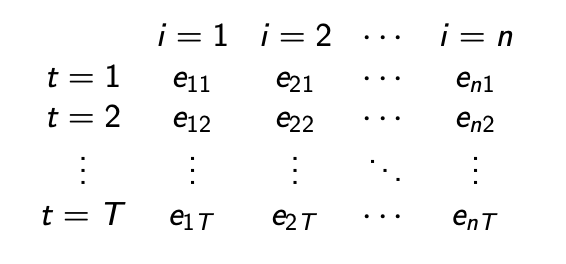
\includegraphics[scale=0.5]{figure1.png}
\end{center}
\textbf{Cross sectional independence:}
\newline
We suppose that $(e_{i1}, e_{i2}, \cdots e_{iT})$ is independent of $(e_{j1}, e_{j2}, \cdots e_{jT})$: cross sectional independence:
\newline
\newline
we control for time-varying common factors with dummies and hope this is enough to capture all sources of cross sectional dependence in the error term.
\newline
\newline
\textbf{time series dependence}
\newline
but we allow for arbitrary dependence for each individual: for each $i$
\begin{equation*}
\begin{aligned}
Cov(e_{it}, e_{is}) \ne 0 \ \ \ \ \textmd{if} \ \ \ t \ne s
\end{aligned} 
\end{equation*}
here, the idea is that even after controlling for individual FE (the $\alpha_i$ ), there is some residual serial dependence we need to account for. \textcolor{NavyBlue}{FE is still unbiased (if all the other assumptions hold, in particular, the exogeneity assumption).However, the standard errors are no longer valid.One way to proceed is to compute robust standard errors}
\subsection{“Clustered standard errors”}
\begin{shaded*}
\noindent Let:
\begin{equation*}
\begin{aligned}
y_{it} = \mu + e_{it} \ \ \ \ \ i=1,\cdots n , t = 1, \cdots T
\end{aligned} 
\end{equation*}
$\mu = E(y_{it})$ is we assume $E(e_{it}) =0$ 
\newline
\newline
The OLS estimator of $\mu$ is :
\begin{equation*}
\begin{aligned}
\hat{\mu} = \frac{1}{Tn} \sum^T_{t=1} \sum^n_{i=1} y_{it}
\end{aligned} 
\end{equation*}
the sample analogue of $\mu$
\newline
\newline
We can rewrite $\hat \mu$ as 
\begin{equation*}
\begin{aligned}
\hat{\mu} = \frac{1}{n} \sum^n_{i=1} (\frac{1}{T} \sum^T_{t=1} y_{it} ) = \frac{1}{n} \sum^n_{i=1} \bar y_i
\end{aligned} 
\end{equation*}
Under cross sectional independence, $(\bar y_1, \bar y_2, \cdots \bar y_n)$ is a random sample and we can apply a CLT to
\begin{equation*}
\begin{aligned}
\hat{\mu} - \mu = \frac{1}{n} \sum^n_{i=1} (\bar y_i - \mu)
\end{aligned} 
\end{equation*}
In particular, if $n \rightarrow \infty$:
\begin{equation*}
\begin{aligned}
\sqrt{n} (\hat{\mu} - \mu) \overset{d}{\rightarrow} N(0,V)
\end{aligned} 
\end{equation*}
where:
\begin{equation*}
\begin{aligned}
V = Var(\sqrt{n} \hat{\mu}) = Var(\frac{1}{\sqrt{n}} \sum^n_{i=1} \bar y_i ) = \frac{1}{n} \sum^n_{i=1} Var(\bar y_i) = Var(\bar y_i)
\end{aligned} 
\end{equation*}
\newline
\newline
The natural estimator is the sample variance of $(\bar y_1, \bar y_2, \cdots \bar y_n):$
\begin{equation*}
\begin{aligned}
\hat{V}= \frac{1}{n} \sum^n_{i=1} (\bar y_i - \bar y)^2
\end{aligned} 
\end{equation*}
where 
\begin{equation*}
\begin{aligned}
\bar y = \frac{1}{n} \sum^n_{i=1} \bar y_i = \frac{1}{nT} \sum^n_{i=1} \sum^T_{t=1} y_{it}
\end{aligned} 
\end{equation*}
By a LLN:
\begin{equation*}
\begin{aligned}
p \ \ \underset{n \rightarrow \infty}{\lim} \ \hat{V} = Var(\bar y_i) \equiv V
\end{aligned} 
\end{equation*}
\end{shaded*}
\subsubsection{Theory of clustered SE}
Clustered SE:
\begin{equation*}
\begin{aligned}
SE_{\hat{\mu}} = \sqrt{\frac{\hat{V}}{n}} = \sqrt{\frac{1}{n} \sum^n_{i=1} (\bar y_i - \bar y)^2 }
\end{aligned} 
\end{equation*}
This estimator is robust to autocorrelation in $y_{it}$
\begin{enumerate}
    \item \textcolor{NavyBlue}{we only used the independence across individuals to derive it.}
    \item we did not specify the presence or absence of serial correlation in $y_{it}$ for each $i$ 
    \item thus, this estimator is valid (i.e. consistent) for any arbitrary form of serial correlation among the observations for each individual.
\end{enumerate}
It is called a “clustered SE” because we view each individual $i$ as a “cluster”:
\begin{itemize}
    \item The observations within each cluster are arbitrarily correlated but we assume the clusters to be independent.
\end{itemize}
\begin{equation*}
\begin{aligned}
V = Var(\bar y_i ) =& \  Var(\frac{1}{T} \sum^T_{t=1} y_{it} ) \\
=& \ \frac{1}{T^2} \sum^T_{t=1} \sum^T_{s=1} Cov(y_{it}, y_{is}) \\
=& \ \frac{1}{T^2} \{ \sum^T_{t=1} Var(y_{it}) + 2 \sum_{s < t} Cov(y_{it}, y_{is}) \}
\end{aligned} 
\end{equation*}
\begin{itemize}
    \item If $y_{it}$ is not autocorrelated, all the autocovariances are zero.
    \item Otherwise, we need to add the autocovariances
    \newline
    If there is positive autocorrelation, the usual estimator (which ignores autocorrelation) will tend to underestimate the true variance
\end{itemize}
\subsubsection{The magic of the clustered SE}
By working with the time averages for each $i$, the clustered SE are automatically robust to serial correlation in $y_{it}$
\begin{equation*}
\begin{aligned}
\hat{V}_{cluster} =& \  \widehat{Var}(\bar y_i) = \frac{1}{n} \sum^n_{i=1} (\bar y_i - \bar y)^2  = \frac{1}{n} \sum^n_{i=1}(\frac{1}{T} \sum^T_{t=1} (y_{it} - \bar y))^2 \\
=& \ \frac{1}{n} \sum^n_{i=1} (\frac{1}{T^2} \sum^T_{t=1} \sum^T_{s=1} (y_{it} - \bar y)(y_{is} - \bar y)) \\
= & \ \frac{1}{T^2} \sum^T_{t=1} \sum^T_{s=1} (\frac{1}{n} \sum^n_{i=1} (y_{it} - \bar y)(y_{is} - \bar y))
\end{aligned} 
\end{equation*}
In contrast, the “usual” estimator omits all the cross products for $t \ne s$ 
\subsection{Asymptotic distribution of the FE estimator for the simple panel regression model}
\begin{center}
\fcolorbox{white}{c1}{\parbox{1\linewidth}{
Consider the simple panel regression model:
\begin{equation*}
\begin{aligned}
y_{it} = \alpha_i + x_{it} \beta +e_{it}
\end{aligned} 
\end{equation*}
where $x_{it}$ is scalar (i.e., $k=1$)
\begin{itemize}
    \item Within transformation:
\end{itemize}
\begin{equation*}
\begin{aligned}
\ddot y_{it} = \ddot x_{it} \beta + \ddot e_{it}
\end{aligned} 
\end{equation*}
\begin{itemize}
    \item The FE of $\beta$:
\end{itemize}
\begin{equation*}
\begin{aligned}
\hat{\beta} = (\sum^n_{i=1} \sum^T_{t=1} (\ddot x_{it})^2)^{-1} \sum^n_{i=1} \sum^T_{t=1} \ddot x_{it} \ddot y_{it}
\end{aligned} 
\end{equation*}
The asymptotic distribution of $\hat{\beta}$ as $n \rightarrow \infty$ and $T$ is fixed:
\begin{equation*}
\begin{aligned}
\sqrt{n} (\hat{\beta} - \beta) =& \  ( \frac{1}{n} \sum^n_{i=1} \frac{1}{T} \sum^T_{t=1} (\ddot x_{it})^2 )^{-1} \frac{1}{\sqrt{n}} \sum^n_{i=1} \frac{1}{T} \sum^T_{t=1} \ddot x_{it}  e_{it} \\
=& \ (\frac{1}{n} \sum^n_{i=1} \bar S_{xx,i})^{-1} \frac{1}{\sqrt{n}} \sum^n_{t=1} \bar S_{xe,i} \\
\textmd{where} \ \ \ \bar S_{xx,i} =& \frac{1}{T} \sum^T_{t=1} (\ddot x_{it})^2 \ \ \ \ \ \textmd{and} \ \ \ \ \bar S_{xe,i} = \frac{1}{T} \sum^T_{t=1} \ddot x_{it} e_{it}
\end{aligned} 
\end{equation*}
Under the cross sectional independence assumption, $(\bar S_{xx,i}, \bar S_{xe,i})$ are jointly independent across $i$. \textcolor{NavyBlue}{So, we can apply LLN's and CLT's for independent data}
}}
\end{center}
\subsubsection{Asymptotic distribution}
Under the assumption that $E(\ddot x_{it} e_{it})=0$
\begin{equation*}
\begin{aligned}
E(\bar S_{xe,i}) = \frac{1}{T} \sum^T_{t=1} E(\ddot x_{it} e_{it} ) = 0
\end{aligned} 
\end{equation*}
This requires strict exogeneity since $\ddot x_{it} = x_{it} - \bar x_i$ and $\bar x_i = T^{-1} \sum^T_{t=1} x_{it}$
\newline
\newline
The variance of $\frac{1}{\sqrt{n}} \sum^n_{i=1} \bar S_{xe,i}: $
\newline
\newline
Under cross sectional independence and $E(\bar S_{xe,i}) = 0$
\begin{equation*}
\begin{aligned}
V = Var(\frac{1}{\sqrt{n}} \sum^n_{i=1} \bar S_{xe,i}) = Var(\bar S_{xe,i}) = E(\bar S_{xe,i}^2)
\end{aligned} 
\end{equation*}
Since $\bar S_{xe,i} = \frac{1}{T} \sum^T_{t=1} \ddot x_{it} e_{it}$
\begin{equation*}
\begin{aligned}
V = E[(\frac{1}{T} \sum^T_{t=1} \ddot x_{it} e_{it} )^2] = \frac{1}{T^2} \sum^T_{t=1} \sum^T_{s=1} E(\ddot x_{it}  e_{it}  \ddot x_{is} e_{is})
\end{aligned} 
\end{equation*}
\textcolor{NavyBlue}{Without the assumption of no serial correlation in $e_{it}$ , we need cluster standard errors}
\newline
\newline
The clustered variance estimator is the sample variance of $\bar S_{x \hat{e},i} = \frac{1}{T} \sum^T_{t=1} \ddot x_{it} \hat{e}_{it}$ where $\hat{e}_{it} = \ddot y_{it} - \ddot x_{it} \hat{\beta}$
\begin{equation*}
\begin{aligned}
\hat{V}_{cluster} = \frac{1}{n} \sum^n_{i=1} (\bar S_{x\hat{e},i})^2 = \frac{1}{n} \sum^n_{i=1} \frac{1}{T^2} \sum^T_{t=1} \sum^T_{s=1} \ddot x_{it} \ddot x_{is} \hat{e}_{it} \hat{e}_{is}
\end{aligned} 
\end{equation*}
\subsubsection{Clustered standard errors}
\begin{equation*}
\begin{aligned}
\sqrt{n} (\hat{\beta} - \beta)
=\ (\frac{1}{n} \sum^n_{i=1} \bar S_{xx,i})^{-1} \frac{1}{\sqrt{n}} \sum^n_{t=1} \bar S_{xe,i} \ \ \ \overset{d}{\rightarrow} N(0,(E(\bar S_{xx,i}))^{-2} V)
\end{aligned} 
\end{equation*}
A natural estimator of $E(\bar S_{xx,i})$ is the sample average $n^{-1} \sum^n_{i=1} \bar S_{xx,i}$
\newline
\newline
The \textcolor{NavyBlue}{clustered variance estimator of $\hat{\beta}$} is given by 
\begin{equation*}
\begin{aligned}
\widehat{Var}(\sqrt{n} \hat{\beta} ) = (n^{-1} \sum^n_{i=1} \bar S_{xx,i})^{-2} \ \ \hat{V}_{\textmd{cluster}}
\end{aligned} 
\end{equation*}
\section{Generalized Least Squares (GLS)}
\begin{shaded*}
\noindent Consider the linear regression model: 
\begin{equation*}
\begin{aligned}
y = X \beta + e, \ \ \ E(e|X) =0 \ \ \ \ Var(e|X) = \Omega
\end{aligned} 
\end{equation*}
When the errors are conditionally homoskedastic and uncorrelated(i.e., $\Omega = \sigma^2 I$), the OLS estimator is BLUE (Gauss-Markov Theorem)
\newline
\newline
When $\Omega$ is of a general form, $\hat{\beta}_{\textmd{OLS}}$ is nolonger efficient
\newline
\newline
The BLUE estimator is given by the GLS estimator:
\begin{equation*}
\begin{aligned}
\hat{\beta}_{\textmd{GLS}} = (X' \Omega^{-1} X)^{-1} X' \Omega^{-1} y
\end{aligned} 
\end{equation*}
\end{shaded*}
\subsection{Derivation of the GLS formula}
Let $Var(e|X)= \Omega$, where \textcolor{NavyBlue}{$\Omega$ is a symmetric positive definite matrix.}
\newline
\newline
$\Rightarrow$ there exists a \textcolor{NavyBlue}{nonsingular matrix $C$} such that:
\begin{equation*}
\begin{aligned}
\underset{n \times n}{\Omega}^{-1} = \underset{n \times n}{C}C'
\end{aligned} 
\end{equation*}
one way to obtain $C$ is to apply the Choleski decomposition, which yields a triangular matrix $C$.
\newline
\newline
Given $C$, we can transform the original model by pre-multiplying it by $C'$:
\begin{equation*}
\begin{aligned}
C'y =& \ C' X \beta + C'e \ \ \ \textmd{or equivalently} \\
y^* =& \ X^* \beta + e^*
\end{aligned} 
\end{equation*}
\textbf{The transformed model satisfies the Gauss-Markov assumptions.}
\subsection{Mean and variance of the transformed error vector}
Transformed model: $y^* = X^* \beta + e^*$ 
\newline
Since $E(e|X)=0:$ 
\begin{equation*}
\begin{aligned}
E(e^*|X^*) =& \  E(C'e|X) = C'E(e|X) = 0 \\ 
\Rightarrow Var(e^* | X^*) =& \ Var(C'e|X) = C'Var(e|X)C \\
=& \ C' \Omega C \\
=& \ C'(\Omega^{-1})^{-1} C \\
=& \ C' (CC')^{-1} C \\
=& \ C'(C')^{-1} C^{-1} C \\
=& \ I_n
\end{aligned} 
\end{equation*}
which is of the type $\sigma^2 I$
\subsection{GLS estimator}
The GLS estimator of $\beta$ is the OLS estimator applied to the transformed model:
\begin{equation*}
\begin{aligned}
\hat{\beta}_{\textmd{GLS}}=& \ (X^{*'} X^*)^{-1} X^{*'} y^* \\
=& \ ((C'X)' (C'X))^{-1} (C'X)'C'y \\
=& \ (X'CC'X)^{-1} X'CC'y \\
=& \ (X' \Omega^{-1} X)^{-1} X' \Omega^{-1} y
\end{aligned} 
\end{equation*}
This estimator is BLUE by the Gauss-Markov Theorem.
\subsection{GLS objective function and special cases of GLS}
\begin{shaded*}
\noindent $\hat{\beta}_{\textmd{GLS}}$ minimizes the following objective function:
\begin{equation*}
\begin{aligned}
Q(\beta) =& (y^* - X^* \beta)' (y^* - X^* \beta) \\
=& (y- X\beta)' CC' (y- X\beta) \\
=& (y-X\beta)' \Omega^{-1} (y- X\beta)
\end{aligned} 
\end{equation*}
This objective function is a generalization of the OLS objective function: $(y-X\beta)' (y-X\beta)$
\begin{itemize}
    \item Thus, OLS is a special case of GLS, where. $\Omega = I_n$
\end{itemize}
\newline
\newline
\textbf{Another special case}: WLS, where $\Omega = \textmd{diag}(\sigma_i^2), \sigma^2_i = Var(e_i|X)$
\newline
Here $Q(\beta)$ is the SSR of weighted observations: $Q(\beta) = e^{*'} e^* = \sum^n_{i=1} (\frac{y_i - x'_i \beta}{\sigma_i})^2$, hence the name "weighted least squares"
\end{shaded*}
\subsection{GLS and Feasible GLS (FGLS)}
The formula:
\begin{equation*}
\begin{aligned}
\hat{\beta}_{\textmd{GLS}} = (X' \Omega^{-1} X)^{-1} X' \Omega^{-1} y
\end{aligned} 
\end{equation*}
is not feasible in general since we don't observe $\Omega$.
\newline
\newline
When we replace $\Omega$ with an estimator $\hat{\Omega}$, we get the FGLS:
\begin{equation*}
\begin{aligned}
\hat{\beta}_{\textmd{FGLS}} = (X' \hat{\Omega}^{-1} X)^{-1} X' \hat{\Omega}^{-1} y
\end{aligned} 
\end{equation*}
\textcolor{NavyBlue}{Unfortunately, the finite sample properties of $\hat{\beta}_{\textmd{FGLS}}$ are not known. 
\begin{itemize}
    \item Even if GLS is BLUE, this is not generally true for FLGS.
    \item asymptotically, FGLS is more efficient than OLS if we correctly specify $\Omega$
\end{itemize}}
\subsection{Random effects}
Let:
\begin{equation*}
\begin{aligned}
y_{it} = \alpha_i + x_{it}' \beta + e_{it}
\end{aligned} 
\end{equation*}
\textbf{To obtain a consistent estimator of $\beta$:}
\newline
we need to eliminate $\alpha_i$ before applying OLS because they might be correlated with $x_{it}$. So far, there are two possible transformations:
\begin{itemize}
    \item FD
    \item FE
\end{itemize}
However, \textcolor{NavyBlue}{if we are willing to assume that $\alpha_i$ is uncorrelated with $x_{it}$} , then a more efficient estimator exists.
\newline
\newline
Another advantage with respect to FE/FD is that we can include time invariant regressors such as gender or race.
\subsection{Homoskedastic equi-correlation structure}
Let
\begin{equation*}
\begin{aligned}
y_{it} = x_{it}' \beta + v_{it}
\end{aligned} 
\end{equation*}
where $v_{it} = e_{it} + \alpha_i$ This \textcolor{NavyBlue}{error term is
autocorrelated} due to the presence of $\alpha_i$
\newline
\newline
Suppose that $e_{it} \sim \textmd{i.i.d.}(0, \sigma^2_e), \alpha_i \sim \textmd{i.i.d.} (0, \sigma^2_\alpha)$ and $e_{it} \perp \alpha_i$
\begin{equation*}
\begin{aligned}
var(v_{it}) =& \ \sigma_e^2 + \sigma_\alpha^2 \\
cov(v_{it}, v_{is})=& \ \sigma_\alpha^2
\end{aligned} 
\end{equation*}
\begin{itemize}
    \item \textcolor{NavyBlue}{the error term is homoskedastic and positively autocorrelated.}
    \item \textcolor{NavyBlue}{the autocorrelation is constant, so we have equi-correlation.}
\end{itemize}
\textbf{Consequences for pooled OLS:}
\begin{enumerate}
    \item the standard errors obtained from OLS are wrong.
    \item OLS is not the best estimator; there is a more efficient estimator: GLS.
\end{enumerate}
\subsubsection{The model in matrix form}
Let: 
\begin{equation*}
\begin{aligned}
y_{it} = x'_{it} \beta + v_{it}
\end{aligned} 
\end{equation*}
where $v_{it} = e_{it} + \alpha_i$ is the composite error. 
\newline
\newline
Stacking the $T$ observations for each $i$ yields:
\begin{equation*}
\begin{aligned}
y_{i} =& x'_{i} \beta + v_{i} \ \ \ \ \ i=1\cdots n \\
& \textmd{where} \\
\underset{T \times 1}{y_i} =& \begin{pmatrix}
y_{i1} \\
\vdots \\
y_{iT}
\end{pmatrix} \ \ \ \ 
\underset{T \times k}{x_i} = \begin{pmatrix}
x_{i1}' \\
\vdots \\
x_{iT}'
\end{pmatrix} \ \ \ \ \textmd{and} \ \ \  \underset{T \times 1}{v_i} = \begin{pmatrix}
v_{i1} \\
\vdots\\
v_{iT}
\end{pmatrix}
\end{aligned} 
\end{equation*}
Letting $\iota_T = (1,\cdots 1)'$ we can write $v_i = e_i + \alpha_i \iota_T$
\newline
\newline
Stacking across $i$ yields:
\begin{equation*}
\begin{aligned}
y =& X \beta + v  \\
& \textmd{where} \\
\underset{nT \times 1}{y} =& \begin{pmatrix}
y_{1} \\
\vdots \\
y_{n}
\end{pmatrix} \ \ \ \ 
\underset{nT \times k}{X} = \begin{pmatrix}
x_{1} \\
\vdots \\
x_{n}
\end{pmatrix} \ \ \ \ \textmd{and} \ \ \  \underset{nT \times 1}{v} =& \begin{pmatrix}
v_{1} \\
\vdots\\
v_{n}
\end{pmatrix} = \begin{pmatrix}
e_1 + \alpha_1 \iota_T \\
\vdots \\
e_n + \alpha_n \iota_T
\end{pmatrix}
\end{aligned} 
\end{equation*}
\subsubsection{RE assumptions}
Under the RE assumptions, $E(v|X)=0$ 
\begin{itemize}
    \item this follows from strict exogeneity (i.e. $E(e_{it}|X)=0$)
    \item independence between fixed effects and regressors (in fact, it suffices that $E(\alpha_i|X)=0$
\end{itemize}
\textcolor{NavyBlue}{$\Rightarrow$ pooled OLS is unbiased.} 
\newline
\newline
Under the typical RE assumptions that
\begin{equation*}
\begin{aligned}
e_{it}|X \sim \textmd{i.i.d.} (0, \sigma_e^2) , \ \ \alpha_i|X \sim \textmd{i.i.d.}(0, \sigma_\alpha^2) \ \ \ \ \ \ \textmd{and} \ \ \ \ \ e_{it} \perp \alpha_i
\end{aligned} 
\end{equation*}
In this case, we will be able to see that $\Omega = E(vv'|X)$ is not of the "ideal" type $\sigma^2 I$ 
\newline
\textcolor{NavyBlue}{$\Rightarrow$ pooled OLS is inefficient}
\subsubsection{Variance-covariance matrix of the error term}
\begin{equation*}
\begin{aligned}
\Omega \equiv E(vv'|X) = \begin{pmatrix}
E(v_1 v_1'|X) & \cdots & E(v_1 v_n'|X) \\
\vdots & \ddots & \vdots \\
E(v_n v_1' |X) & \cdots & E(v_n v_n'|X)
\end{pmatrix}
\end{aligned} 
\end{equation*}
Under the RE assumptions, $E(v_i v_j'|X)=0$ for $i \ne j$ and 
\begin{equation*}
\begin{aligned}
E(v_i v_i'|X) =& \begin{pmatrix}
E(v_{i1}^2|X) & \cdots & E(v_{i1}v_{iT}|X) \\
\vdots & \ddots & \vdots \\
E(v_{iT}v_{i1}|X) & \cdots & E(v_{iT}^2|X)
\end{pmatrix} \\
=& \begin{pmatrix}
\sigma_e^2 + \sigma_\alpha^2 & \cdots & \sigma_\alpha^2 \\
\vdots & \ddots & \vdots \\
\sigma_\alpha^2 & \cdots & \sigma_e^2 + \sigma_\alpha^2
\end{pmatrix}
\end{aligned} 
\end{equation*}
$\Rightarrow \ \ \Omega$ is block diagonal...OLS is not BLUE. 
\newline
\textcolor{NavyBlue}{The RE estimator is the GLS estimator in this model.}
\subsection{The random effects estimator}
Panel data model in matrix form:
\begin{equation*}
\begin{aligned}
y = X \beta + v \ \ \ \ E(v|X)=0 \ \ \ \ \ \textmd{and} \ \ \ \ E(vv'|X)=\Omega
\end{aligned} 
\end{equation*}
Under the homoskedastic and equi-correlated structure of the errors:
\begin{equation*}
\begin{aligned}
\underset{nT \times nT}{\Omega} = \textmd{diag}(\Sigma) \ \ \ \textmd{where} \ \ \ \underset{T \times T}{\Sigma} = \begin{pmatrix}
\sigma_e^2 + \sigma_\alpha^2 & \cdots & \sigma_\alpha^2 \\
\vdots & \ddots & \vdots \\
\sigma_\alpha^2 & \cdots & \sigma_e^2 + \sigma_\alpha^2
\end{pmatrix}
\end{aligned} 
\end{equation*}
where $\sigma_e^2 = Var(e_{it})$ and $\sigma_\alpha^2 = Var(\alpha_i)$
\begin{itemize}
    \item The RE estimator is the FGLS estimator
\end{itemize}
\begin{equation*}
\begin{aligned}
\hat{\beta}_{\textmd{RE}} = (X' \hat{\Omega}^{-1} X)^{-1} X' \hat{\Omega}^{-1} y
\end{aligned} 
\end{equation*}
where $\hat{\Omega} = \textmd{diag}(\hat{\Sigma})$. This requires $\hat{\sigma}_e^2$ and $\hat{\sigma}_\alpha^2$
\subsection{Feasible GLS estimation}
Note that: $e_{it} = y_{it} - \alpha_i - \beta' x_{it}$, we can estimate:
\begin{equation*}
\begin{aligned}
\hat{e}_{it} = y_{it} - \hat{\alpha}_i - \hat{\beta}x_{it} = (y_{it} - \bar y_i ) - (x_{it} - \bar x_i)' \hat{\beta} = \widehat{\ddot e_{it}}
\end{aligned} 
\end{equation*}
where $\hat{\beta}$ is the FE estimator of $\beta$ and we let $\hat{\alpha_i} = \bar y_i - \hat{\beta}' \bar x_i$
\begin{equation*}
\begin{aligned}
\Rightarrow \ \ \ \hat{\sigma}_2 = 
\frac{1}{n(T-1)-k}\sum^T_{t=1} \sum^n_{i=1} \widehat{\ddot e_{it}}^2
\end{aligned} 
\end{equation*}
the number of degrees of freedom is $nT-n-k=n(T-1)-k$,since we have to estimate $n$ individual effects and $k$ parameters in $\beta$
\newline
\newline
\textbf{A popular estimator is based on the "between" regression:}
\begin{equation*}
\begin{aligned}
\bar y_i = \bar x_i' \beta + \alpha_i + \bar e_i \ \ \ \ i=1,2\cdots , n
\end{aligned} 
\end{equation*}
This estimator is unbiased and consistent under the same assumptions as RE
\newline
\newline
we have that
\begin{equation*}
\begin{aligned}
Var(\bar u_i) = Var(\alpha_i) + Var(\bar e_i) = \sigma_\alpha^2 + \frac{1}{T} \sigma_e^2
\end{aligned} 
\end{equation*}
Implying that:
\begin{equation*}
\begin{aligned}
\hat{\sigma}^2_\alpha =& \widehat{Var(\bar u_i)} - \frac{1}{T} \hat{\sigma}_e^2 \\
\widehat{Var(\bar{u}_i)} =& \frac{1}{n-k} \sum^n_{i=1} (\bar y_i - \bar x_i' \hat{\beta}_{\textmd{between}})^2
\end{aligned} 
\end{equation*}
\chapter{Chapter 3}
\section{Generalized Method of Moments}
Consider the linear regression model: $y_i = x_i' \beta + e_i$ 
\newline
\textcolor{NavyBlue}{The most important assumption for OLS is $E(x_i e_i)=0$. Without it, OLS is not even consistent.}
\subsection{Simultaneity bias: demand and supply of oranges in Florida}
\textcolor{Purple}{
The variables $q_i$ and $p_i$ (quantity and price) are jointly determined by the demand equation
\begin{equation*}
\begin{aligned}
q_i = \alpha_0 + \alpha_1 p_i + e_{1i} \ \ \ \ \ \textmd{(demand)} 
\end{aligned} 
\end{equation*}
and the supply equation
\begin{equation*}
\begin{aligned}
q_i = \beta_0 + \beta_1 p_i + e_{2i} \ \ \ \ \ \textmd{(supply)} 
\end{aligned} 
\end{equation*}
where $\alpha_1 \ne \beta_1$
\newline
\newline
Economic theory predicts that $\alpha_1< 0$ and $\beta_1 >0$.
\newline
The error term $e_{1i}$ contains all the factors that determine the demand
for oranges other than the price ("demand shifters": e.g. preference for oranges).
\newline
Similarly, $e_{2i}$ contains the "supply shifters": e.g., the temperature.}
\newline
\newline
Suppose that
\begin{equation*}
\begin{aligned}
e_{1i} \sim \textmd{i.i.d.} (0, \sigma_1^2) \ \ \ \ \ e_{2i} \sim \textmd{i.i.d.}(0, \sigma_2^2), \ \ \ E(e_{1i} e_{2i}) = 0
\end{aligned} 
\end{equation*}
\subsubsection{The reduced form equations}
\textcolor{Purple}{
If we equate demand=supply,
\begin{equation*}
\begin{aligned}
\alpha_0 + \alpha_1 p_i + e_{1i} =& \beta_0 + \beta_1 p_i + e_{2i} \\
p_i =& \frac{\alpha_0 - \beta_0}{\beta_1 - \alpha_1} + \frac{e_{1i}-e_{2i}}{\beta_1 - \alpha_1} \ \ \ \ \ (3)
\end{aligned} 
\end{equation*}}
which implies that:
\begin{equation*}
\begin{aligned}
q_i =& \beta_0 + \beta_1 (\frac{\alpha_0 - \beta_0}{\beta_1 - \alpha_1} + \frac{e_{1i}-e_{2i}}{\beta_1 - \alpha_1}) + e_{2i} \\
=& \frac{\beta_1 \alpha_0 - \beta_0 \alpha_1}{\beta_1 - \alpha_1} + \frac{\beta_1}{\beta_1 -  \alpha_1}e_{1i} - \frac{\alpha_1}{\beta_1 - \alpha_1} e_{2i} \ \ \ \ \ (4)
\end{aligned} 
\end{equation*}
(3) and (4) are called the reduced form equations:
\begin{itemize}
    \item they express each endogenous variable as a function of exogenous variables (here, $e_{1i}$ and $e_{2i}$ ).
\end{itemize}
\subsubsection{Endogeneity of price and quantity}
Suppose we would like to estimate the demand equation:
\begin{equation*}
\begin{aligned}
q_i = \alpha_0 + \alpha_1 p_i + e_{1i}
\end{aligned} 
\end{equation*}
Using the reduced form equation of $p_i:$
\begin{equation*}
\begin{aligned}
Cov(p_i, e_{1i}) = \frac{\sigma_1^2}{\beta_1 - \alpha_1} \ne 0
\end{aligned} 
\end{equation*}
i.e. pi is endogenous in demand
\newline
\newline
Similarly
\begin{equation*}
\begin{aligned}
Cov(p_i, e_{2i}) = - \frac{\sigma_2^2}{\beta_1 - \alpha_1} \ne 0
\end{aligned} 
\end{equation*}
and therefore $p_i$ is endogenous in the supply equation
\subsubsection{The probability limit of the OLS estimator of the price effect coefficient}
The OLS estimator of regressing $q_i$ on $p_i$ :
\begin{equation*}
\begin{aligned}
\hat{\theta}_1 = \frac{n^{-1}\sum^n_{i=1}(p_i - \bar p)q_i}{n^{-1}\sum^n_{i=1}(p_i - \bar p)^2} \overset{P}{\rightarrow} \frac{Cov(p_i,q_i)}{Var(p_i)} \equiv \theta_1
\end{aligned} 
\end{equation*}
$\theta_1$ is the linear projection coefficient in the model
\begin{equation*}
\begin{aligned}
q_i = \theta_0 + \theta_1 p_i + v_i \ \ \ \ \ Cov(p_i, v_i)=0
\end{aligned} 
\end{equation*}
We have that:
\begin{equation*}
\begin{aligned}
Cov(p_i,q_i) =& Cov(\frac{e_{1i}-e_{2i}}{\beta_1 - \alpha_1}, \frac{\beta_1}{\beta_1 - \alpha_1}e_{1i} - \frac{\alpha_1}{\beta_1 - \alpha_1} e_{2i}) \\
=& \frac{\beta_1}{(\beta_1 - \alpha_1)^2} \sigma_1^2 + \frac{\alpha_1}{(\beta_1 - \alpha_1)^2} \sigma_2^2 \\
Var(p_i) =& \frac{\sigma_1^2 + \sigma_2^2}{(\beta_1 - \alpha_1)^2}
\end{aligned} 
\end{equation*}
\textbf{The limit in probability of the OLS estimator:}
\begin{equation*}
\begin{aligned}
\theta_1 \equiv p \ \lim \hat{\theta}_1 = \frac{\beta_1 \sigma_1^2 + \alpha_1 \sigma_2^2}{\sigma_1^2 + \sigma_2^2}
\end{aligned} 
\end{equation*}
In general, $\theta_1$ is different from $\beta_1$ and $\alpha_1$. We have a simultaneity bias.
\begin{itemize}
    \item If $\sigma_1^2 =0$ (i.e., no "demand shifters"), then $p \lim \hat{\theta}_1 = \alpha_1$. i.e., we estimate the demand equation
    \item If $\sigma_2^2 =0$ (i.e., no "supply shifters"), then $p \lim \hat{\theta}_1 = \beta_1$. i.e., we estimate the supply equation
\end{itemize}
This analysis suggests that we can estimate the demand equation if we find a variable that affects the supply but not the demand equation.
\subsubsection{Identification of the demand equation: observable supply shifters}
Suppose we can decompose the supply shock $e_{2i}$ into an observable factor $t_i$. (e.g. temperature) and an unobservable factor $\epsilon_{2i}$
\begin{equation*}
\begin{aligned}
e_{2i} = \beta_2 t_i + \epsilon_{2i}
\end{aligned} 
\end{equation*}
where $\beta_2 \ne 0$ is such that $Cov(t_i, \epsilon_{2i}) =0$ (i.e., $\beta_2$ is a linear projection
coefficient).
\newline
\newline
Then, we obtain the following system of equations
\begin{equation*}
\begin{aligned}
q_i =& \ \alpha_0 + \alpha_1 p_i + e_{1i} \ \ \ \ \textmd{demand} \\
q_i =& \ \beta_0 + \beta_1 p_i + \beta_2 t_i + \epsilon_{2i} \ \ \ \ \textmd{supply}
\end{aligned} 
\end{equation*}
Under certain conditions, we will be able to use $t_i$ as an instrumental variable for $p_i$ in the demand equation.
\subsection{Conditions on the instrumental variable}
\begin{shaded*}
\noindent Two condition:
\begin{enumerate}
    \item $Cov(t_i, e_{1i}) =0$ (exogeneity of the instrument)
    \item $Cov(t_i,p_i) \ne 0$ (relevance of the instrument
\end{enumerate}
The first condition requires that $t_i$ does not determine the demand of oranges (this is something we must assume).
\newline
\newline
The second condition is verified if $\beta_2 \ne 0$
\begin{itemize}
    \item This is the identification condition.
    \item We can test this assumption using the reduced form equation.
\end{itemize}
\end{shaded*}
\subsubsection{The reduced form equations}
We can solve the system with respect to $(q_i,p_i)$ to find:
\begin{equation*}
\begin{aligned}
p_i =& \frac{\alpha_0 - \beta_0}{\beta_1 - \alpha_1} - \frac{\beta_2}{\beta_1 - \alpha_2} t_i + \frac{e_{1i}- \epsilon_{2i}}{\beta_1 - \alpha_1} \ \ \ \ \ (5)\\
q_i =& \frac{\alpha_0 \beta_1 - \alpha_1 \beta_0 }{\beta_1 - \alpha_1} - \frac{\alpha_1 \beta_2}{\beta_1 - \alpha_1}t_i + \frac{\beta_1}{\beta_1 -  \alpha_1}e_{1i} - \frac{\alpha_1}{\beta_1 - \alpha_1} \epsilon_{2i} 
\end{aligned} 
\end{equation*}
Since $Cov(t_i, e_{1i})=0$ and $Cov(t_i, \epsilon_{2i} =0$
\begin{equation*}
\begin{aligned}
Cov(t_i, p_i) = - \frac{\beta_2}{\beta_1 - \alpha_1} Var(t_i) \ne 0
\end{aligned} 
\end{equation*}
if $\beta_2 \ne 0$
\newline
\newline
$\Rightarrow$ Thus, $t_i$ is a valid instrument for $p_i$ in the demand equation. 
\subsubsection{Instrumental variable estimator}
Consider the demand equation: $q_i = \alpha_0 + \alpha_1 p_i + e_{1i}$
\newline
We have that:
\begin{equation*}
\begin{aligned}
Cov(t_i, q_i) =& \ Cov(t_i, \alpha_0 + \alpha_1 p_i + e_{1i}) \\
=& \ \alpha_1 Cov(t_i,p_i) + Cov(t_i, e_{1i}) \\
=& \ \alpha_1 Cov(t_i , p_i) \ \ \ \ \textmd{Since} \ \ Cov(t_i, e_{1i}) = 0
\end{aligned} 
\end{equation*}
Because $Cov(t_i, p_i) \ne 0$, it follows that:
\begin{equation*}
\begin{aligned}
\alpha_1 = \frac{Cov(t_i,q_i)}{Cov(t_i,p_i)}
\end{aligned} 
\end{equation*}
A consistent etimator of $\alpha_1$ is: 
\begin{equation*}
\begin{aligned}
\hat{\alpha}_1 = \frac{\widehat{Cov}(t_i,q_i)}{\widehat{Cov}(t_i,p_i)} = \frac{n^{-1}\sum^n_{i=1}(t_i - \bar t)(q_i - \bar q)}{n^{-1} \sum^n_{i=1} (t_i - \bar t)(p_i - \bar p)}
\end{aligned} 
\end{equation*}
\textcolor{Purple}{
\begin{itemize}
    \item Other examples of endogeneity bias
    \begin{itemize}
        \item Omission of relevant explanatory variables: OVB problem.
        \item Presence of measurement error in explanatory variables: the "errors-in-variables problem".
    \end{itemize}
\end{itemize}
}
\subsubsection{Errors-in-variables problem}
Suppose we would like to estimate a consumption function:
\begin{equation*}
\begin{aligned}
y_i = \beta_0 + \beta_1 x_i^* + e_i
\end{aligned} 
\end{equation*}
where $y_i$ is consumption and $x_i^*$ is income. Assume that this model satisfies the Gauss-Markov assumptions, so in particular
\begin{equation*}
\begin{aligned}
Cov(x_i^*, e_i) =0
\end{aligned} 
\end{equation*}
However, we observe reported income, i.e., we observe
\begin{equation*}
\begin{aligned}
x_i = x_i^* + v_i
\end{aligned} 
\end{equation*}
where $v_i$ is a measurement error.
\newline
\textcolor{NavyBlue}{Depending on the assumptions we make on $v_i$, we might have an endogeneity problem for the observed regressor $x_i$}
\begin{itemize}
    \item A natural assumption is $E(e_i|x_i^*,x_i)=0$
\end{itemize}
This implies that $E(y_i|x_i^*,x_i)=E(y_i|x_i^*)$, i.e. consumption depends only on actual income. Adding the measured income does not change the expectation
\begin{itemize}
    \item Classical error-in-variable assumption: $v_i$ is uncorrelated with $x_i^*$
    \begin{enumerate}
        \item measurement error in income is assumed uncorrelated with actual income
        \item this assumption might be questionable
        \item under this assumption, we can show that $x_i$ is correlated with the error term of the underlying regression.
    \end{enumerate}
\end{itemize}
\subsubsection{Attenuation bias}
To see the endogeneity problem, replace $x_i^* = x_i-v_i$ into the original equation
\begin{equation*}
\begin{aligned}
y_i =& \beta_0 + \beta_1 x_i + (-\beta_1 v_i + e_i) \\
\newline
\newline
Cov(x_i, u_i) =& - \beta_1 Cov(x_i, v_i) + Cov(x_i, e_i) = -\beta_1 \sigma_v^2 \ne 0
\end{aligned} 
\end{equation*}
Let $\hat{\beta}_1= \frac{\sum^n_{i=1}(x_i - \bar x)y_i}{\sum^n_{i=1}(x_i - \bar x)^2}$ be the OLS estimator. Then:
\begin{equation*}
\begin{aligned}
p \ \lim \hat{\beta}_1 = \beta_1 + \frac{Cov(x_i,u_i)}{Var(x_i)} = \beta_1 + \frac{- \beta_1 \sigma^2_v}{\sigma_{x*}^2 + \sigma_v^2} = \beta_1 ( \frac{\sigma_{x*}^2}{\sigma_{x*}^2 + \sigma_v^2})
\end{aligned} 
\end{equation*}
Thus, the estimated OLS is attenuated (or biased towards zero): if $\beta_1 >0$ , we obtain $\hat{\beta}_1 < \beta_1$ and if $\beta_1 <1, \hat{\beta}_1 > \beta_1$
\subsection{Instrumental variable estimator: one single regressor and one single instrument}
Consider:
\begin{equation*}
\begin{aligned}
y_i = \beta_1 + \beta_2 x_{2i} + e_i
\end{aligned} 
\end{equation*}
where $E(e_i)=0$ and
\begin{equation*}
\begin{aligned}
Cov(e_i, x_{2i} ) = E(x_{2i} e_i) \ne 0
\end{aligned} 
\end{equation*}
i.e., $x_{2i}$ is an endogenous regressor
\newline
\newline
$z_{2i}$ is an IV for $x_{2i}$ if it is excluded from previous function and 
\begin{equation*}
\begin{aligned}
Cov(z_{2i},e_i) =& E(z_{2i} e_i)=0 \ \ \ \ \ (7) \\
Cov(z_{2i}, x_{2i} ) \ne& \ 0 \ \ \ \ \ (8)
\end{aligned} 
\end{equation*}
The condition (8) is an identification condition (rank condition)
\subsubsection{Derivation of the IV estimator}
Given that $y_i = \beta_1 + \beta_2 x_{2i} + e_i$
\begin{equation*}
\begin{aligned}
Cov(z_{2i}, y_i) =& \ Cov(z_{2i}, \beta_1 + \beta_2 x_{2i} + e_i) \\
=& \ \beta_2 \ Cov(z_{2i}, x_{2i}) + Cov(z_{2i}, e_i)
\end{aligned} 
\end{equation*}
Thus: 
\begin{equation*}
\begin{aligned}
\beta_2 = \frac{Cov(z_{2i}, y_i)}{Cov(z_{2i},x_{2i})}
\end{aligned} 
\end{equation*}
The IV estimator of $\beta_2$ is:
\begin{equation*}
\begin{aligned}
\hat{\beta}_{2,IV} = \frac{n^{-1}\sum^n_{i=1} (z_{2i}-\bar z_i)(y_i -\bar y)}{n^{-1} \sum^n_{i=1} (z_{2i} - \bar z_2 )(x_{2i} - \bar x_2)}
\end{aligned} 
\end{equation*}
\subsubsection{Convergence of IV}
By a LLN:
\begin{equation*}
\begin{aligned}
p \ \lim \ \hat{\beta}_{2,IV} =& \ \beta_2 + \frac{plim \ n^{-1}\sum^n_{i=1}(z_{2i}-\bar z_2)e_i}{plim \ n^{-1} \sum^n_{i=1} (z_{2i} - \bar z_2)(x_{2i} - \bar x_2)} \\
=& \ \beta_2 + \frac{Cov(z_{2i},e_i)}{Cov(z_{2i}, x_{2i})} \\
=& \beta_2
\end{aligned} 
\end{equation*}
Thus, $\hat{\beta}_{2,IV}$ is a consistent estimator of $\beta_2$, by construction (because we assumed that $Cov(z_{2i},e_i)=0$ and $Cov(z_{2i},x_{2i}\ne 0)$
\newline
\newline
To consistently estimate $\beta_1$ we can use the condition:
\begin{equation*}
\begin{aligned}
E(e_i)= 0 \Leftrightarrow E(y_i - \beta_1 - \beta_2 x_{2i} ) = 0 \Leftrightarrow \beta_1 = E(y_i) - \beta_2 E(x_{2i})
\end{aligned} 
\end{equation*}
which implies
\begin{equation*}
\begin{aligned}
\hat{\beta}_{1,IV} = \bar y - \hat{\beta}_{2,IV} \bar x_2
\end{aligned} 
\end{equation*}
as in OLS (but with the difference that we use $\hat{\beta}_{2,IV}$ instead of $\hat{\beta}_{2,OLS}$
\subsubsection{Testing the identification condition:}
We can test $H_0: Cov(z_{2i},x_{2i})=0$ with a t-test on $\pi_2$ in the linear projection model:
\begin{equation*}
\begin{aligned}
x_{2i} = \pi_1 = \pi_2 z_{2i} + v_i \ \ \ \ \ \ E(v_i) =0 \ \ \ \ E(z_{2i}v_i) =0
\end{aligned} 
\end{equation*}
where:
\begin{equation*}
\begin{aligned}
\pi_2 = \frac{Cov(z_{2i},x_{2i})}{Var(z_{2i})}
\end{aligned} 
\end{equation*}
In particular:
\begin{equation*}
\begin{aligned}
H_0 :& \  \pi_2 = 0 \Leftrightarrow Cov(z_{2i}, x_{2i})= 0 \\
vs H_1:& \ \pi_2 \ne 0 \Leftrightarrow Cov(z_{2i}, x_{2i} ) \ne 0
\end{aligned} 
\end{equation*}
where the test statistic is:
\begin{equation*}
\begin{aligned}
t_{\hat{\pi}_2} = \frac{\hat{\pi}_2}{se(\hat{\pi}_2)}
\end{aligned} 
\end{equation*}
We can use a robust standard error
\subsection{Asymptotic properties of IV}
Let
\begin{equation*}
\begin{aligned}
y_i =& \beta_1 + \beta_2 x_{2i} + e_i \ \ \ \ \ \textmd{where} \\
E(e_i) =& 0 \ \ \ \ E(z_{2i} e_i) =0
\end{aligned} 
\end{equation*}
and assume that $\{ (y_i, x_{2i},z_{2i}:i=1,\cdots, n\}$ is i.i.d.
\newline
\newline
The IV estimator of $\beta_2$ is
\begin{equation*}
\begin{aligned}
\hat{\beta}_2 = \frac{\sum^n_{i=1}(z_{2i}-\bar z_2)y_i}{\sum^n_{i=1}(z_{2i}- \bar z_2)(x_{2i}-\bar x_2)} = \beta_2 + \frac{\sum^n_{i=1}(z_{2i}-\bar z_2)e_i}{\sum^n_{i=1}(z_{2i}-\bar z_2)(x_{2i}-\bar x_2)}
\end{aligned} 
\end{equation*}
after we replace $y_i$
\begin{itemize}
    \item The asymptotic variance of $\hat{\beta}_2$
\end{itemize}
\begin{equation*}
\begin{aligned}
V_{\hat{\beta}_2} = \frac{Var((z_{2i}-\mu_{z_2})e_i)}{(Cov(z_{2i},x_{2i}))^2}
\end{aligned} 
\end{equation*}
\begin{itemize}
    \item The asymptotic variance under homoskedasticity
\end{itemize}
Suppose that $E(e_i^2|z_{2i}) = \sigma^2$ (this is the homoskedasticity condition under IV)
\begin{equation*}
\begin{aligned}
Var((z_{2i} - \mu_{z_2} )e_i) =& \ E((z_{2i} - \mu_{z_2})^2 e_i^2) \\
=& \ E((z_{2i}- \mu_{z_2})^2 E(e_i^2 | z_{2i})) \\
=& \ \sigma^2 Var(z_{2i})
\end{aligned} 
\end{equation*}
And:
\begin{equation*}
\begin{aligned}
V_{\hat{\beta}_2} = \frac{Var((z_{2i}-\mu_{z_2})e_i)}{(Cov(z_{2i}, x_{2i}))^2}= \frac{\sigma^2 Var(z_{2i})}{[Cov(z_{2i},x_{2i})]^2}
\end{aligned} 
\end{equation*}
\begin{shaded*}
\begin{itemize}
    \item \textbf{Comparison of the asymtotic variance of OLS and IV}
\end{itemize}
We can write:
\begin{equation*}
\begin{aligned}
V_{\hat{\beta}_{2,IV}} \equiv Var(\sqrt{n} \hat{\beta}_{2,IV}) = \frac{\sigma^2}{\rho^2_{z2,x2}Var(x_{2i})}
\end{aligned} 
\end{equation*}
where
\begin{equation*}
\begin{aligned}
\rho_{z2,x2} = Cov(z_{2i}, x_{2i}) / \sqrt{Var(x_{2i})} \sqrt{Var(z_{2i})}
\end{aligned} 
\end{equation*}
is the correlation coefficient between the instrument and the regressor
\newline
\newline
In contrast:
\begin{equation*}
\begin{aligned}
V_{\hat{\beta}_{2,OLS}} \equiv Var(\sqrt{n} \hat{\beta}_{2,OLS}) = \frac{\sigma^2}{Var(x_{2i})}
\end{aligned} 
\end{equation*}
Since $\rho^2_{z_2,x_2} \le 1$ , $V_{\hat{\beta}_{2,IV}} \ge V_{\hat{\beta}_{2,OLS}}$
\newline
\newline
Thus, the IV standard errors are larger than those of OLS
\begin{itemize}
    \item \textbf{Consistent estimation of the asymptotic variance}
\end{itemize}
The estimator of $\sigma^2$ is
\begin{equation*}
\begin{aligned}
\hat{\sigma^2} = \frac{1}{n-2} \sum^n_{i=1} \hat{e_i}^2 
\end{aligned} 
\end{equation*}
where $\hat{e}_i = y_i - \hat{\beta}_{1,IV} - \hat{\beta}_{2,IV} x_{2i}$
\newline
\newline
The estimator of $\rho^2_{z_2,x_2}$ is the $R^2$ from regressing $x_2$ on $z_2$ (inclusing a constant):
\begin{equation*}
\begin{aligned}
R^2_{x_2,z_2} = ( \widehat{Cov} (z_{2i}, x_{2i}) / \sqrt{\widehat{Var}(x_{2i})} \sqrt{\widehat{Var}(z_{2i}}))^2
\end{aligned} 
\end{equation*}
The estimator of $Var(x_{2i})$ is the sample variance of $x_2$:
\begin{equation*}
\begin{aligned}
\widehat{Var}(x_{2i})
\end{aligned} 
\end{equation*}
\begin{itemize}
    \item \textbf{Consistent estimator of V}
\end{itemize}
We obtain the following estimator:
\begin{equation*}
\begin{aligned}
\hat{V}_{\hat{\beta}_{2,IV}} \equiv& \  \widehat{Var}(\sqrt{n} \hat{\beta}_{2,VI})  \\
=& \ \frac{\hat{\sigma}^2}{R^2_{z_2,x_2} \widehat{Var}(x_{2i})}
\end{aligned} 
\end{equation*}
Thus, the estimated variance of $\hat{\beta}_{2,IV}$ is:
\begin{equation*}
\begin{aligned}
\widehat{Var}(\hat{\beta}_{2,IV}) = \frac{\sigma^2}{R^2_{z_2,x_2}\times SST_{x_2}} \ \ \ \ \ \ SST_{x_2} = \sum^n_{i=1} (x_{2i} - \bar x_2)^2
\end{aligned} 
\end{equation*}
This is a decreasing function of $R^2_{x_2,z_2}$ i.e., the weaker the correlation between the IV and the endogenous variable, the larger the standard error of $\hat{\beta}_{2,IV}$
\end{shaded*}
\subsubsection{Problem caused by "weak instruments"}
The $IV \ z_{2i}$ is "weak" if $Cov(z_{2i},x_{2i})$ is weak:
\begin{itemize}
    \item The standard errors of IV are "very large" 
    \item The standard normal distribution is not a good approximation to the finite sampling distribution of the IV estimator 
    \item inference based on the normal critical values is not correct
\end{itemize}
\subsubsection{Consequences of weak IV on bias}
If $Cov(z_{2i},e_i)$ is not exactly null, the IV estimator is no longer consistent
\newline
\newline
Indeed:
\begin{equation*}
\begin{aligned}
p \ \lim \hat{\beta}_{2,IV} = \beta_2 + \frac{Cov(z_{2i},e_i)}{Cov(z_{2i},x_{2i}} = \beta_2 + \frac{\sigma_e}{\sigma_{x_2}} \frac{Corr(z_{2i},e_i)}{Corr(z_{2i},x_{2i})}
\end{aligned} 
\end{equation*}
This shows that $p \ \lim \hat{\beta}_{2,IV} - \beta_2$ can be very large if $Corr(z_{2i}, x_{2i}) \approx 0$, even if $Corr(z_{2i},e_i) \approx 0$, but not quite zero
\newline
\newline
The IV estimator can be even more biased than OLS estimator. Indeed:
\begin{equation*}
\begin{aligned}
p \ \lim \hat{\beta}_{2,OLS} = \beta_2 + \frac{Cov(x_{2i},e_i)}{Var(x_{2i})} = \beta_2 + \frac{\sigma_e}{\sigma_{x_2}} Corr(x_{2i},e_i)
\end{aligned} 
\end{equation*}
The comparison between the two biases depends on the maginitutde of $\frac{Corr(z_{2i},e_i)}{Corr(z_{2i},x_{2i})}$ and $Corr(x_{2i},e_i)$
\subsection{A general linear regression model}
Consider the linear regresion model
\begin{equation*}
\begin{aligned}
y_i = x_i' \beta + e_{i}
\end{aligned} 
\end{equation*}
where $x_i$ is a $k \times 1$ vector such that $E(x_i e_i)\ne 0$
\newline
\newline
Among the $k$ regressors, $k_1$ are exogenous and $k_2$ are endogenous, i.e., if:
\begin{equation*}
\begin{aligned}
\underset{k \times 1}{x_i} = \begin{pmatrix}
x_{1i} \\
x_{2i}
\end{pmatrix} \begin{matrix}
k_1 \times 1 \\
k_2 \times 1
\end{matrix} \ \ \ \ \ \ k_1 + k_2 = k
\end{aligned} 
\end{equation*}
we have that $E(x_{1i}e_i) =0$ but $E(x_{2i}e_i) \ne 0$ and thus
\begin{equation*}
\begin{aligned}
E(x_i e_i ) = E(\begin{bmatrix} x_{1i}e_i \\ x_{2i}e_i \end{bmatrix} ) \ne 0
\end{aligned} 
\end{equation*}
\subsection{The general case: several instruments and several endogenous regressors}
Let $z_i$ denote a vector of $\ell$ random variables such that $E(z_i e_i)=0$ 
\newline
\newline
We can paritition $z_i$ as follows:
\begin{equation*}
\begin{aligned}
\underset{\ell \times 1}{z_i} = \begin{pmatrix}
z_{1i} \\
z_{2i}
\end{pmatrix} =\begin{pmatrix}
x_{1i} \\
z_{2i}
\end{pmatrix} \ \ \ \begin{matrix}
k_1 \times 1 \\
\ell_2 \times 1
\end{matrix} \ \ \ \ \ \ k_1 + \ell_2 = \ell
\end{aligned} 
\end{equation*}
Because $E(x_{1i}e_i) = 0$, the elements of $x_{1i}$ are included in $z_i$
\newline
\newline
The variables $z_{1i} = x_{1i}$ are included exogenous variables whereas $z_{2i}$ are excluded exogenous variables
\newline
\newline
So far, $k_2 = \ell_2 =1$ i.e., one single instrument for one single regressor
\begin{itemize}
    \item Now we are going to consider $\ell_2 . k_2$
    \begin{enumerate}
        \item we will first consider estimation in the just identified case where $\ell_2 = k_2$
        \item and then move to the overidentified case, where $\ell_2 > k_2$
    \end{enumerate}
\end{itemize}
\textcolor{Purple}{
\textbf{Example: Return to Schooling}
\newline
\newline
Consider estimating the returns to schooling $(\beta_2)$ using a model such as 
\begin{equation*}
\begin{aligned}
\log (\textmd{wages}_i) =& \  \beta_1 + \beta_2 \textmd{educ}_i + \beta_3 \textmd{experience}_i + \beta_4 \textmd{experience}_i^2 + e_i \\
y_i =& \ \log (\textmd{wage}_i) , \ \ \ k=4 \\
x_i =& \begin{pmatrix}
1 \\
\textmd{experience}_i \\
\textmd{experience}_i^2 \\
\textmd{educ}_i
\end{pmatrix} \ \ \ \ \begin{matrix}
k_1 =3 \\
k_2 =1
\end{matrix}
\end{aligned} 
\end{equation*}
where $\textmd{educ}_i$ is potentially endogenous as it depends on ability
\newline
\newline
Assuming experience is exogenous, we need to find at least one instrument.
\newline
\newline
Card (1995): use college proximity to instrument for education: if a
person lives close to a college, this reduces the cost of attendance and increases the likelihood the person will attend college. At the same time, whether someone lives close to a college does not determine his/her ability, so no direct impact on wages.}
\subsection{A general linear IV regression model}
Consider the linear regression model:
\begin{equation*}
\begin{aligned}
y_i = x_i' \beta + e_i
\end{aligned} 
\end{equation*}
where $x_i$ is a $k \times 1$ vector such taht $E(x_ie_i)\ne 0$ 
\newline
\newline
We have an $\ell \times 1$ vector $z_i$ such that:
\begin{equation*}
\begin{aligned}
E(z_i e_i) =0 
\end{aligned} 
\end{equation*}
\subsection{Identification}
The moment conditions define a system of $\ell$ linear equations in $k$ unknowns:
\begin{equation*}
\begin{aligned}
E(z_ie_i)= E(z_i(y_i - x_i'\beta)) = 0
\end{aligned} 
\end{equation*}
or:
\begin{equation*}
\begin{aligned}
E(z_ix'_i)\beta = E(z_iy_i)
\end{aligned} 
\end{equation*}
By assumption, there exists at least one value of $\beta$ that solves this system
\newline
\newline
Identification means that there is only one such value
\newline
From linear algebra, a necessary and sufficient condition is that rank $(E(z_ix_i'))=k$
\subsubsection{The rank identification condition}
To ensure that a unique $\beta$ solves the moment conditions, we impose:
\begin{equation*}
\begin{aligned}
rank(E(z_ix_i'))=k
\end{aligned} 
\end{equation*}
\begin{itemize}
    \item Special case: $\ell=k$
\end{itemize}
In this case, $E(z_ix_i')$ is a square matrix and the rank condition implies that $\beta= E(z_i x_i')^{-1} E(z_iy_i)$
\begin{itemize}
    \item More generally, the rank condition requires $\ell \ge k$
\end{itemize}
This is because for any $\ell \times k$ matrix $A$, rank(A) $\le \min(\ell, k)$
\newline
$\Rightarrow$  if $\ell < k$, then $rank(E(z_ix_i'))$ would have to be smaller or equal than $\ell$, contradicting the rank condition. 
\subsubsection{The order condition for identification}
The order condition simply states that $\ell \ge k$. This is a necessary but not sufficient condition for identification
\newline
\newline
It requires that:
\begin{equation*}
\begin{aligned}
\# \ \textmd{moment (orthogonality) conditions} \ge& \  \# \  \textmd{parameters, or}. \\
\# \ \textmd{instruments} \ge& \  \# \  \textmd{regressors,  or} \\
\# \ \textmd{excluded exogenous variables} \ge& \  \# \ \textmd{endogenous regressors}
\end{aligned} 
\end{equation*}
Suppose the rank condition is satisfied. Then:
\begin{itemize}
    \item the model is just or exactly identified if $\ell =k$ 
    \item the model is over-identified if $\ell > k$ 
\end{itemize}
If $\ell <k$ (or the rank condition is not satisfied), we say the model is not identified(or under-identified)
\newline
\newline
\textcolor{Purple}{
\textbf{An example: simple linear regression with one instrument only:}
\newline
\newline
Simple linear regression model: $y_i = x_i' \beta + e_i$, where $E(e_i)=0$ and
\begin{equation*}
\begin{aligned}
x_i = \begin{pmatrix}
1 \\ 
x_{2i}
\end{pmatrix} \ \ \ \ \ \ \ \beta = \begin{pmatrix}
\beta_1 \\
\beta_2
\end{pmatrix}
\end{aligned} 
\end{equation*}
Only one instrumental variable: $z_{2i}$
\newline
\newline
Moment conditions: $E(e_i)=0$ and $E(z_{2i} e_i) =0 $. Letting:
\begin{equation*}
\begin{aligned}
\underset{2 \times 1}{z_i} = \begin{pmatrix}
1 \\
z_{2i}
\end{pmatrix}
\end{aligned} 
\end{equation*}
We can write the moment conditions as $E(z_ie_i)=0$ \newline
\newline
Here $\ell = k =2$
\newline
\newline
We have that:
\begin{equation*}
\begin{aligned}
E \underset{2 \times 2}{(z_ix_i')} = E( \begin{pmatrix}
1 \\ 
z_{2i}
\end{pmatrix} \ \ \ \begin{pmatrix}
1 & x_{2i}
\end{pmatrix}) = \begin{pmatrix}
1 & E(x_{2i}) \\
E(z_{2i}) & E(z_{2i} x_{2i})
\end{pmatrix}
\end{aligned} 
\end{equation*}
For a square matrix, requiring that the columns are linearly independent is equivalent to requiring that the matrix is nonsingular, i.e.
\begin{equation*}
\begin{aligned}
det(E(z_i x_i')) \ne 0
\end{aligned} 
\end{equation*}
This is equivalent to:
\begin{equation*}
\begin{aligned}
Cov(z_{2i}, x_{2i}) = E(z_{2i} x_{2i} ) - E(z_{2i}) E(x_{2i}) \ne 0
\end{aligned} 
\end{equation*}
which is exactly the identification condition we have before
\begin{itemize}
    \item The rank condition is a generalization of this condition
\end{itemize}}
\subsubsection{Instrumental variables estimator in the just identified case}
Let 
\begin{equation*}
\begin{aligned}
y_i = x_i' \beta + e_i = x_{1i}' \beta_1 + x_{2i}' \beta_2 + e_i
\end{aligned} 
\end{equation*}
\begin{itemize}
    \item $x_i' = (x_{1i}', x_{2i}'$ is $1 \times k$, where $k=k_1 + k_2$
    \item $x_{1i}$ are $k_1$ exogenous regressors
    \item $x_{2i}$ are $k_2$ endogenous regressors
\end{itemize}
Assume that we have a vector of $\ell = k$ moment conditions: 
\begin{equation*}
\begin{aligned}
E(z_ie_i) = E(\begin{pmatrix}
x_{1i} \\
z_{2i}
\end{pmatrix} \ e_i ) = 0
\end{aligned} 
\end{equation*}
$z_{2i}$ is $\ell_2 \times 1$ with $\ell_2 = k_2$
\newline
\newline
\textbf{Estimate $\beta$ consistently:}
\newline
The simple formula of IV we say up to now only applies when $\ell = k =2$ i.e. when $\ell_2 = k_2 =1:$
\begin{equation*}
\begin{aligned}
\hat{\beta}_{IV} = \frac{\sum^n_{i=1}(z_{2i}- \bar z_2)y_i}{\sum^n_{i=1}(z_{2i} - \bar z)(x_{2i} - \bar x_2)}
\end{aligned} 
\end{equation*}
We seek a generalization of this formula that applies for any values of $\ell$ and $k$ satisfying $\ell = k$
\begin{itemize}
    \item Making the substitution $e_i = y_i - x_i' \beta$, we find
\end{itemize}
\begin{equation*}
\begin{aligned}
E(z_i (y_i - x'_i \beta)) =& \  0 \\
\textmd{or} \\
E(z_i y_i) - E(z_i x'_i)\beta =& \  0
\end{aligned} 
\end{equation*}
where $E(z_i x'_i)$ is a square matrix when $\ell = k$
\begin{itemize}
    \item Solving for $\beta$ gives
\end{itemize}
\begin{equation*}
\begin{aligned}
\beta = (E(z_i x'_i))^{-1} E(z_i y_i)
\end{aligned} 
\end{equation*}
This assumes invertibility of $E(z_i x'_i)$, which holds under the rank condition
\begin{itemize}
    \item The IV estimator for $\beta$ replaces the population moments by their sample versions:
\end{itemize}
\begin{equation*}
\begin{aligned}
\hat{\beta}_{iv} =& \  (n^{-1} \sum^n_{i=1} z_i x'_i)^{-1} n^{-1} \sum^n_{i=1} z_i y_i \\
=& \  (\sum^n_{i=1} z_i x'_i)^{-1} \sum^n_{i=1} z_i y_i \\
=& \ (Z'X)^{-1} Z' y
\end{aligned} 
\end{equation*}
Here:
\begin{equation*}
\begin{aligned}
\underset{n \times k}{Z} = \begin{pmatrix}
x'_{1i} & z'_{2i}
\end{pmatrix} \textmd{and} \underset{n \times k}{X} = \begin{pmatrix}
x_{1i}' & x'_{2i}
\end{pmatrix}
\end{aligned} 
\end{equation*}
\subsubsection{Instrumental variables estimator in general case}
The \textcolor{NavyBlue}{previous fomular} only applies when $k = \ell$ 
\begin{itemize}
    \item can't invert the $\ell \times k$ matrix $(Z'X)$ when $\ell > k$ (not a square matrix)
\end{itemize}
How should we estimate $\beta$ when $\ell > k \ ?$ 
\begin{itemize}
    \item In Cardís example, we might consider proximity to a public college and proximity to a private college.
    \item Or we might use motherís and fatherís education to instrument for a personís level of education.
\end{itemize}
One consistent estimator is the two-stage-least-squares (2SLS) estimator.
\begin{itemize}
    \item this estimator "works" whenever $\ell \ge k$ 
    \item it amounts to the previous IV estimator when $\ell =k$ 
    \item when $\ell > k$, it is the most efficient IV estimator (under a certain
    homoskedasticity assumption).
\end{itemize}
\textcolor{Purple}{
\textbf{Example:}
\newline
\newline
Consider
\begin{equation*}
\begin{aligned}
\log (\textmd{wages}_i) =& \  \beta_1 + \beta_2 \textmd{educ}_i + \beta_3 \textmd{expereince}_i + \beta_4 \textmd{experience}_i^2 + e_i \\
y_i =& \  \log(\textmd{wage}_i) \ \ \ \ k =4 \\
x_i =& \begin{pmatrix}
1 \\
\textmd{experience}_i \\
\textmd{experience}_i^2 \\
\textmd{educ}_i
\end{pmatrix} \ \ \ \ \begin{matrix}
k_1 =3 \\
k_2 =1
\end{matrix}
\end{aligned} 
\end{equation*}
and $\ell =5$
\begin{equation*}
\begin{aligned}
z_i = \begin{pmatrix}
x_{1i} \\ z_{2i}
\end{pmatrix} \ \ \ = \begin{pmatrix}
1 \\
\textmd{experience}_i \\
\textmd{experience}_i^2 \\
\textmd{father educ}_i \\
\textmd{mother educ}_i
\end{pmatrix} \ \ \ \ \ \begin{matrix}
k_1 =3 \\
I_2 = 2
\end{matrix}
\end{aligned} 
\end{equation*}
We estimate the reduced form equation for educ:
\begin{equation*}
\begin{aligned}
\textmd{educ}_i = \pi_i + \pi_2 \textmd{experience}_i + \pi_3 \textmd{experience}_i^2 + \pi_4 \textmd{father educ}_i + \pi_5 \textmd{mother educ}_i + v_i
\end{aligned} 
\end{equation*}
and we get:
\begin{equation*}
\begin{aligned}
\widehat{\textmd{educ}_i} = \hat{\pi}_1 + \hat{\pi}_2 \textmd{experience}_i + \hat{\pi}_3 \textmd{experience}_i^2 + \hat{\pi}_4 \textmd{father educ}_i + \hat{\pi}_5 \textmd{mother educ}_i
\end{aligned} 
\end{equation*}
We estimate the following regression by OLS
\begin{equation*}
\begin{aligned}
\log (\textmd{wage}_i) = \beta_1 + \beta_2 \widehat{\textmd{educ}_i} + \beta_3 \textmd{experience}_i + \beta_4 \textmd{experience}_i^2 + r_i
\end{aligned} 
\end{equation*}}
\textbf{Why does this work ? }
\newline
Take the simple case where:
\begin{equation*}
\begin{aligned}
y_i = \beta_1 + \beta_2 x_{1i} + \beta_3 x_{2i} + e_i
\end{aligned} 
\end{equation*}
where $x_{1i}$ is exogenous and $x_{2i}$ is endogenous
\newline
\newline
we have two instruments $z_{2i}$ and $z_{3i}$
\newline
\newline
Take the reduced form equation for $x_{2i}:$
\begin{equation*}
\begin{aligned}
x_{2i} = \pi_1 + \pi_2 x_{1i} + \pi_3 z_{2i} + \pi_4 z_{3i} + v_i
\end{aligned} 
\end{equation*}
where by definition of linear projection 
\begin{equation*}
\begin{aligned}
Cov(x_{2i}^*, v_i) = 0
\end{aligned} 
\end{equation*}
The exogeneity of $x_{1i}, z_{2i}$ and $z_{3i}$ implies:
\begin{equation*}
\begin{aligned}
Cov(x_{2i}^*,  e_i) = Cov(\pi_1 + \pi_2 x_{1i} + \pi_3 z_{2i} + \pi_4 z_{3i}, e_i) =0
\end{aligned} 
\end{equation*}
By replacing $x_{2i}$ with $x_{2i}^*+v_i$, we get:
\begin{equation*}
\begin{aligned}
y_i =& \ \beta_1 + \beta_2 x_{1i} + \beta_3 (x_{2i}^* + v_i) + e_i \\
=& \ \beta_1 + \beta_2 x_{1i} + \beta_3 x_{2i}^* + (\beta_3 v_i + e_i) \\
=& \ \beta_1 + \beta_2 x_{1i} + \beta_3 x_{2i}^* + r_i \ \ \ \ \ \ \ \ (3)
\end{aligned} 
\end{equation*}
where 
\begin{equation*}
\begin{aligned}
r_i = \beta_3 v_i + e_i
\end{aligned} 
\end{equation*}
is mean zero and is uncorrelated with $x_i$ and $x_{2i}^*$
\newline
$\Rightarrow$ Thus, we can estimate (3) with OLS
\newline
\newline
\textbf{Note:} \textcolor{NavyBlue}{However that the standard errors of (3) are note valid.} The true variance depends on the variance of $e_i$ whereas the errors of (3) are given by $r_i$
\subsection{Derivation of 2SLS in the general case}
In the general case, we have
\begin{equation*}
\begin{aligned}
y_i = x_i' \beta + e_i
\end{aligned} 
\end{equation*}
where $x_i$ is $k \times 1$
\newline
\newline
The reduced form equations for $x_i$ can be written as 
\begin{equation*}
\begin{aligned}
\underset{k \times 1}{x_i} = \underset{k \times \ell}{\Pi}' z_i + \underset{k \times 1}{v_i} \ \ \ \ \ \textmd{where} E(z_i v_i') = 0_{\ell \times k}
\end{aligned} 
\end{equation*}
\begin{itemize}
    \item $E(z_iv_i') =0$ is not an assumption: it follows by definition of the linear projection matrix $\Pi$
    \item In particular, we can show that if $\Pi$ is defined by:
\end{itemize}
\begin{equation*}
\begin{aligned}
\Pi = E(z_i z_i')^{-1} E(z_i x_i')
\end{aligned} 
\end{equation*}
then $E(z_i v_i') =0$. The model equations are: 
\begin{equation*}
\begin{aligned}
y_i =& \ x_i' \beta + e_i \\
x_i =& \ \Pi' z_i + v_i
\end{aligned} 
\end{equation*}
By definition of linear projection $E(z_i v_i')=0$. Replacing $x_i$ with $\Pi'z_i + v_i$ in the structural equation for $y_i$ yields:
\begin{equation*}
\begin{aligned}
y_i = (z_i' \Pi)\beta + (e_i + v_i' \beta)
\end{aligned} 
\end{equation*}
where
\begin{equation*}
\begin{aligned}
E(z_i r_i) =0
\end{aligned} 
\end{equation*}
Since
\begin{equation*}
\begin{aligned}
E(z_i e_i) = 0 \ \ \ (\textmd{by the exogeneity assumption on } z_i) \\
E(z_i v_i') = 0 \ \ \ (\textmd{by the linear projection assumption})
\end{aligned} 
\end{equation*}
Let $x_i^* = \Pi' z_i$, we can write
\begin{equation*}
\begin{aligned}
y_i = x_i^{*'} \beta + r_i \ \ \ \ E(x_i^* r_i) = 0
\end{aligned} 
\end{equation*}
If we knew $\Pi$, then we would estimate $\beta$ by least-squares of $y_i$ on $x_i^*$
\begin{equation*}
\begin{aligned}
\hat{\beta} = (X^{*'} X^*)^{-1} X^{*'} y
\end{aligned} 
\end{equation*}
where
\begin{equation*}
\begin{aligned}
\underset{n \times k}{X^*} = \begin{pmatrix}
x_1^{*'} \\
\vdots \\
x_n^{*'}
\end{pmatrix} = \begin{pmatrix}
(\Pi' z_1)' \\
\vdots \\
(\Pi' z_n)'
\end{pmatrix} \ \ \ = \begin{pmatrix}
z_1' \Pi \\
\vdots \\
z_n' \Pi
\end{pmatrix} \ \ \ = Z \Pi
\end{aligned} 
\end{equation*}
Thus, we would get
\begin{equation*}
\begin{aligned}
\hat{\beta} = (\Pi' Z'Z \Pi)^{-1} \Pi' Z'y
\end{aligned} 
\end{equation*}
This estimator is infeasible as it depends on the unknown $\Pi$
\subsection{The 2SLS formula}
\begin{shaded*}
\noindent Since $\Pi = E(z_i z_i')^{-1} E(z_i x_i')$, we estimate $\Pi$ consistently with
\begin{equation*}
\begin{aligned}
\hat{\Pi} = (Z'Z)^{-1} Z'X
\end{aligned} 
\end{equation*}
This implies the 2SLS formula:
\begin{equation*}
\begin{aligned}
\hat{\beta}_{2sls} =& \  (\hat{\Pi}' Z'Z\hat{\Pi})^{-1} \hat{\Pi}' Z' y \\
=& \ (X'Z(Z'Z)^{-1} Z'Z(Z'Z)^{-1} Z'X)^{-1} X'Z(Z'Z)^{-1} Z'y \\
=& \ (X'Z(Z'Z)^{-1} Z'X)^{-1} X'Z(Z'Z)^{-1} Z'y
\end{aligned} 
\end{equation*}
\end{shaded*}
\subsubsection{2SLS reduced to IV when the model is just identified}
Since $\ell =k$, the matrices $(Z'X)$ and $(X'Z)$ are square, and we can factor
\begin{equation*}
\begin{aligned}
(X'Z(Z'Z)^{-1} Z'X)^{-1} =& \ (Z'X)^{-1} ((Z'Z)^{-1})^{-1} (X'Z)^{-1} \\
=& \ (Z'X)^{-1} Z'Z(X'Z)^{-1}
\end{aligned} 
\end{equation*}
It follows that:
\begin{equation*}
\begin{aligned}
\hat{\beta}_{2sls} =& \  (X'Z(Z'Z)^{-1} Z'X)^{-1} X'Z(Z'Z)^{-1} Z'y \\
=& \ (Z'X)^{-1} Z'Z (X'Z)^{-1} X'Z(Z'Z)^{-1} Z'y \\
=& \ (Z'X)^{-1} Z'y \\
=& \hat{\beta}_{IV}
\end{aligned} 
\end{equation*}
Thus, 2SLS is a generalization of the IV estimator defined before
\subsubsection{Alternative representation of 2SLS}
Let 
\begin{equation*}
\begin{aligned}
P_z = Z(Z'Z)^{-1} Z'
\end{aligned} 
\end{equation*}
\begin{itemize}
    \item this is the usual projection matrix on the space generated by the columns of $Z$
    \item when we premultiply any vector by $P_Z$ we obtain the fitted values from regressing that vector on $Z$
\end{itemize}
It follows that
\begin{equation*}
\begin{aligned}
\hat{\beta}_{2sls} =& \  (X'Z(Z'Z)^{-1} Z'X)^{-1} X'Z(Z'Z)^{-1} Z'y \\
=& \ (X'P_Z X)^{-1} X'P_Z y
\end{aligned} 
\end{equation*}
\subsubsection{2SLS at two-step OLS}
Write:
\begin{equation*}
\begin{aligned}
\hat{\beta}_{2sls} =& \  (X'P_Z X)^{-1} X'P_Z y\\
=& \ (X'P'_Z P_ZX)^{-1} X'P'_ZP_Zy \\
=& \ (\hat{X}' \hat{X})^{-1} \hat{X'}y
\end{aligned} 
\end{equation*}
where $\hat{X} = P_Z X$ and where $P_Z$ is symmetric and idempotent
\newline
\newline
This suggest that we can obtain 2SLS in two steps:
\begin{itemize}
    \item Regress $X$ on $Z$ and get "fitted values" $\hat{X} = P_Z X$ 
    \item Regress $y$ on $\hat{X}$ and get $\hat{\beta}_{2sls} = (\hat{X}' \hat{X})^{-1} \hat{X'}y$
\end{itemize}
\subsection{Interpretation of the formula with only one endogenous regressor}
Suppose that $k_2 =1$ and hence:
\begin{equation*}
\begin{aligned}
X =& \  \begin{pmatrix}
\underset{n \times k_1}{X_1} & \underset{n \times 1}{x_2}
\end{pmatrix} \\
Z =& \ \begin{pmatrix}
\underset{n \times k_1}{X_1} & \ \underset{n \times \ell_2}{Z_2}
\end{pmatrix} \ \ \ \ \ell_2 \ge 1
\end{aligned} 
\end{equation*}
Then:
\begin{equation*}
\begin{aligned}
\hat{X} = P_Z \begin{pmatrix}
X_1 & x_2
\end{pmatrix} = \begin{pmatrix}
P_Z X_1 & P_Z x_2
\end{pmatrix} = \begin{pmatrix}
X_1 & \hat{x}_2
\end{pmatrix}
\end{aligned} 
\end{equation*}
Since $X_1$ belongs to $Z$. 
\newline
\newline
Hence, the formula $\hat{\beta}_{2sls}= (\hat{X}'\hat{X})^{-1}\hat{X}'y$ can be interpreted as the OLS estimator in the regression of $y$ on $X_1$ and $\hat{x}_2$, where $\hat{x}_2$ are the fitted values of regressing $x_2$ on $Z$. 
\subsection{The variance-covariance matrix of 2SLS}
write:
\begin{equation*}
\begin{aligned}
\hat{\beta}_{2sls} =& \ (X'P_ZX)^{-1} X'P_Z y\\
=& \ (X'P_Z X)^{-1} X'P_Z (X\beta+e) \\
=& \ \beta + (X' P_Z X)^{-1} X'P_Z e
\end{aligned} 
\end{equation*}
If $Var(e|X,Z)=\sigma^2 I_n$
\begin{equation*}
\begin{aligned}
Var(\hat{\beta}_{2sls}|X,Z) = \sigma^2 (X' P_ZX)^{-1}= \sigma^2 (\hat{X'} \hat{X'})^{-1}
\end{aligned} 
\end{equation*}
The parameter $\sigma^2$ is the variance of the original error term $e$. 
\newline
\newline
A consistent estimator of $\sigma^2$ is
\begin{equation*}
\begin{aligned}
\hat{\sigma}^2 = \frac{(y- X \hat{\beta}_{2sls})'(y-X\hat{\beta}_{2sls})}{n-k}
\end{aligned} 
\end{equation*}
\subsubsection{The 2SLS and the IV estimators}
Consider again the example:
\textcolor{Purple}{
\begin{equation*}
\begin{aligned}
\log (\textmd{wage}_i)= \beta_1 + \beta_2 \textmd{educ}_i + \beta_3 \textmd{experience}_i + \beta_4 \textmd{experience}_i^2 + e_i
\end{aligned} 
\end{equation*}
We have two instruments: \textmd{father educ} and $\textmd{mother educ}_i$
\newline
\newline
\textmd{If we try to use the formula for IV estimator}
\begin{equation*}
\begin{aligned}
\hat{\beta}_{IV} = (Z'X)^{-1} Z'y
\end{aligned} 
\end{equation*}
We have a problem because $Z$ is $n \times 5$ and hence $Z'X$ is $5 \times 4$ (non invertible) 
\newline
\newline
We could however do IV with only one of the instruments. For instance:
\begin{equation*}
\begin{aligned}
Z = (1, \textmd{experience}_i , \textmd{experience}_i^2 , \textmd{father educ}_i)
\end{aligned} 
\end{equation*}
2SLS chooses the best linear combination of the two IV's: $Z = \hat{X}$
\newline
This turns out to be the most efficient IV estimator under homoskedasticity of the error term}
\subsubsection{2SLS is the efficient IV estimator Under the homoskedasticity assumption}
\begin{itemize}
    \item 2SLS
\end{itemize}
\begin{equation*}
\begin{aligned}
\hat{\beta}_{2sls} = (\hat{X}'\hat{X})^{-1} \hat{X}' y
\end{aligned} 
\end{equation*}
where 
\begin{equation*}
\begin{aligned}
\hat{X} = P_Z X
\end{aligned} 
\end{equation*}
and the fitted values from the regression of $X$ on $Z$
\begin{itemize}
    \item Efficient IV:
\end{itemize}
\begin{equation*}
\begin{aligned}
\hat{\beta}_{IV} = (\hat{X}'X)^{-1} \hat{X}' y
\end{aligned} 
\end{equation*}
This is the same formula we saw for the simple case $:(Z'X)^{-1}Z'y$, with $Z= \hat{X}$
\newline
\newline
$\Rightarrow$ we can show that $\hat{\beta}_{2sls} = \hat{\beta}_{IV}$
\newline
Indeed:
\begin{equation*}
\begin{aligned}
\hat{\beta}_{IV} = (\hat{X}' X)^{-1} \hat{X}' y = (X' P'_Z X)^{-1} X'P_Z y =\hat{\beta}_{2sls}
\end{aligned} 
\end{equation*}
\subsubsection{Testing the rank condition in general case: Several endogenous regressors and several instruments}
Suppose we have two instruments for $x_{2i}, z_{2i}$ and $z_{3i}$ 
\begin{itemize}
    \item The reduced from equation for $x_{2i}:$
\end{itemize}
\begin{equation*}
\begin{aligned}
x_{2i} = \pi_1 + \pi_2 x_{1i} + \pi_3 z_{2i} + \pi_4 z_{3i} + v_i
\end{aligned} 
\end{equation*}
\begin{itemize}
    \item To test the rank condition, we can test 
\end{itemize}
\begin{equation*}
\begin{aligned}
H_0 :& \ \pi_3 = \pi_4 = 0 \ vs.  \\
H_1 :& \ \pi_3 \ne 0 \ \ \textmd{or} \ \pi_4 \ne 0
\end{aligned} 
\end{equation*}
\begin{itemize}
    \item An $F-$test is appropriate to test $H_0$ 
\end{itemize}
If we reject $H_0,$ at least one of the two available IV's ($z_{2i}$ or $z_{3i}$ is correlated (partially) with $x_{2i}$ and we can proceed with 2SLS. 
\subsubsection{Testing the rank condition in the general case: Several endogenous regressors and several instruments}
Consider the example
\begin{equation*}
\begin{aligned}
y_i = \beta_1 + \beta_2 x_{1i} + \beta_3 x_{2i}+ \beta_3 x_{3i} + e_i
\end{aligned} 
\end{equation*}
where 
\begin{equation*}
\begin{aligned}
x_{1i} \ \ \ \textmd{is exogenous} \\
x_{2i} \ \textmd{and} x_{3i} \ \textmd{are endogenous}
\end{aligned} 
\end{equation*}
The order condition requires at least two IV, $z_{2i}$ and $z_{3i}$ 
\subsection{Testing for endogeneity}
Consider the model:
\begin{equation*}
\begin{aligned}
y_i= x_{1i}' \beta_1 + x_{2i}' \beta_2 + e_i
\end{aligned} 
\end{equation*}
where $x_{1i}$ is a vector of $k_1$ exogenous variables and $x_2$ is $k_2 \times 1$
\begin{itemize}
    \item We would like to test
\end{itemize}
\begin{equation*}
\begin{aligned}
H_0:  E(x_{2i} e_i) = 0 \ \ \ \ \textmd{vs} \ \ \ H_1: E(x_{2i} e_i) \ne 0 
\end{aligned} 
\end{equation*}
Under $H_0, x_{2i}$ are exogenous $\Rightarrow$ OLS is consistent (and efficient under the Gauss-Markov assumptions); IV is also consistent but inefficient
\newline
\newline
Under $H_1, x_{2i}$ is endogenous and OLS is asymptotically biased. IV is consistent
\begin{itemize}
    \item To test $H_0$ we need instruments. Let
\end{itemize}
\begin{equation*}
\begin{aligned}
z_i = \begin{pmatrix}
x_{1i}\\
z_{2i}
\end{pmatrix} \ \ \begin{matrix}
k_1 \times 1 \\
\ell_2 \times 1
\end{matrix}
\end{aligned} 
\end{equation*}
where $\ell_2 \ge k_2$. We will work under the assumption that $E(z_i e_i)=0$
\subsubsection{Hausman's Test}
The idea is to compare the OLS and the 2SLS estimators:
\begin{equation*}
\begin{aligned}
H = \sqrt{n}(\hat{\beta}_{2SLS} - \hat{\beta}_{OLS})' [\widehat{Var}(\sqrt{n} (\hat{\beta}_{2SLS} - \hat{\beta}_{OLS}))]^{-1} \sqrt{n} (\hat{\beta}_{2SLS} - \hat{\beta}_{OLS})
\end{aligned} 
\end{equation*}
\begin{itemize}
    \item If $H_0$ is true, then the two estimators OLS and 2SLS should be similar
    \item But if $H_0$ is false, $\hat{\beta}_{OLS} \rightarrow^p \beta_{proj}$, the projection coefficient, whereas $\hat{\beta}_{2SLS} \rightarrow^p \beta$. Thus, $H \rightarrow^p \infty$
\end{itemize}
This suggests that we should reject $H_0$ if $H$ is sufficiently large. 
\newline
\newline
We can show that $H$ is asymptotically distributed as a chi-square random variable.
\newline
\textbf{Inverting the var-cov matrix is difficult}
\subsubsection{Steps of the Hausman test(Via an auxiliary regression)}
If we would like to test the endogeneity of a single regressor, e.g. $x_2$ the steps are:
\begin{enumerate}
    \item Estimate the OLS the reduced form equation of this variable and get the residuals $\hat{v}_{2i}:$
\newline
\begin{equation*}
\begin{aligned}
\hat{v}_{2i} = x_{2i} - z_i' \hat{\pi}
\end{aligned} 
\end{equation*}
    \item Estimate by OLS the original model "arugumented" with $\hat{v}_{2i}$:
\newline
\begin{equation*}
\begin{aligned}
y_i = x'_{1i} \beta_1 + x_{2i} \beta_2 + \rho \hat{v}_{2i} + r_i
\end{aligned} 
\end{equation*}
    \item Test:
\newline
\begin{equation*}
\begin{aligned}
H_0 : \rho =  0    \ \ \ \textmd{vs.} \ \ \ \ \ H_1: \rho \ne 0
\end{aligned} 
\end{equation*}
with a $t$-test
\end{enumerate}
If we reject $H_0$, we can conclude that $x_2$ is endogenous
\subsection{Testing the exogeneity of an instrument:Possible only in. the overidentified case}
Let:
\begin{equation*}
\begin{aligned}
y_i = x'_{1i} \beta_1 + x_{2i} \beta_2 + e_i
\end{aligned} 
\end{equation*}
where the variable $x_{2i}$ is endogenous
\begin{itemize}
    \item If we only have an IV, say $z_{2i}$, then the exogeneity hypothesis 
\newline
\begin{equation*}
\begin{aligned}
E(z_{2i} e_i) =0
\end{aligned} 
\end{equation*}
can not be tested
    \item In constrast, if we have several IV, say $z_{2i}$ and $z_{3i}$, we can test if one of them is uncorrelated with $e_i$ maintaining the hypothesis that the other one is exogenous
    \item Intuitively, with two or more IV, we can use one IV to obtain an estimate of $e_i$ (by IV regression) and then check whether $\hat{e_i}$ is correlated with the other IV.
\end{itemize}
\subsubsection{Testing overidentification restrictions}
\begin{itemize}
    \item Suppose that $\ell_2 = \ \#$ instruments $> k_2 = \ \# $ endogenous explanatory variables (the model is overidentified)
    \item The null hypothesis underlying the $J$ test of overidentification (Hansen, 1982) is 
\newline
\begin{equation*}
\begin{aligned}
H_0 : E(z_i e_i)=0 \ \ \ \ell \times 1
\end{aligned} 
\end{equation*}
where
\begin{equation*}
\begin{aligned}
z_i = \begin{pmatrix}
x_{1i} \\
z_{2i}
\end{pmatrix} \ \ \ \ \begin{matrix}
k_1 \times 1 \\
\ell_2 \times 1
\end{matrix} \ \ \ \ \ \ k_1 + \ell_2 = \ell > k_1 + k_2
\end{aligned} 
\end{equation*}
    \item The $J$ test can be written as a quadratic form of the empirical moment conditions
    \item Its symptotic distribution is $\chi^2_{\ell -k}$ under $H_0$
    \begin{itemize}
        \item This requires $\ell >k$
        \item if $\ell =k, J=0$ and we can't test $H_0$
        \item If we reject $H_0$, we conclude that there is at least one IV in the model that is not exogenous (but this test does not allow us to decide which one it is)
    \end{itemize}
\end{itemize}
\subsubsection{Testing for overidentifying restriction using an auxiliary regression}
The $J-$ test can be implemented as follows:
\begin{enumerate}
    \item We estimate the original model by 2SLS and we get the residuals
\begin{equation*}
\begin{aligned}
\hat{e}_i = y_i - x'_i \hat{\beta}_{2SLS} = y_i - x'_{1i} \hat{\beta}_{1,2SLS} - x'_{2i} \hat{\beta}_{2,2SLS} 
\end{aligned} 
\end{equation*}
    \item We regress $\hat{e}_i$ on all the exogenous variables, i.e., we regress $\hat{e}_i $ on 
\begin{equation*}
\begin{aligned}
z_i = \begin{pmatrix}
x'_{1i} & z'_{2i}
\end{pmatrix}'
\end{aligned} 
\end{equation*}
and we get the $R^2$
    \item We compute $J=nR^2$. Under $H_0 : E(z_i e_i)=0, \ \ \ J \rightarrow^d \chi^2_{\ell -k}$
    \begin{itemize}
        \item If $p-$value $(J)<\alpha$, we reject the $H_0$ and we conclude that where are variables in $z_i$ that are not exogenous
    \end{itemize}
\end{enumerate}
\subsection{GMM}
\begin{itemize}
    \item  Generalized method of moments (GMM) is one of the most popular estimation methods in econometrics.
    \item GMM generalizes the method of moment estimators by allowing for models with more equations than unknown parameters (overidentified models).
    \item It includes as special cases OLS, IV, and 2SLS.
\end{itemize}
\subsection{Moment equations models}
\begin{itemize}
    \item The models we have seen so far can all be defined by a set of orthogonality conditions of the type:
\newline
\begin{equation*}
\begin{aligned}
E(\underset{\ell \times 1}{g_i} (\beta)) =0
\end{aligned} 
\end{equation*}
where $g_i(\beta)$ is a known $\ell \times 1$ function of the $i^{th}$ observation and a $k \times 1$ parameter $\beta$ 
\begin{itemize}
    \item for OLS, we let $g_i(\beta) = x_i(y_i - x'_i \beta)$
    \item for IV, we let $g_i(\beta) = z_i (y_i - x'_i \beta)$
\end{itemize}
    \item The parameter $\beta$ is identified if there is a unique solution to this system of equations.
    \item This required $\ell \ge k$, as explained before
    \begin{itemize}
        \item If $\ell <k$, $\beta$ is underidentified (or not identified). This means that there exists more than one solution for the system of equations.
        \item If $\ell =k$, $\beta$ is exactly identified (if a rank condition holds)
        \item If $\ell>k$, $\beta$ is overidentified (if a rank condition holds)
    \end{itemize}
\end{itemize}
\subsection{Method of moments estimator}
Suppose the model is just identified, i.e. $\ell =k$ \begin{itemize}
    \item The method of moments suggests we replace these moment conditions by their sample analogue
\newline
\begin{equation*}
\begin{aligned}
\bar g_n (\beta) = \frac{1}{n} \sum^n_{i=1} g_i (\beta) =0 
\end{aligned} 
\end{equation*}
    \item This gives the method of moments estimator $\hat{\beta}_{mm}:$
\begin{equation*}
\begin{aligned}
\bar g_n (\hat{\beta}_{mm}) = \frac{1}{n} \sum^n_{i=1} g_i (\hat{\beta}_{mm}) = 0
\end{aligned} 
\end{equation*}
    \item For instance, in the linear IV model with as many instruments as moment conditions $\hat{\beta}_{mm} = \hat{\beta}_{IV}$
    \item When $\ell >k$, we have more equations than unknowns and so this is not feasible
    \item In this case, we need to use the Generalized method of moments (GMM) estimator
\end{itemize}
\subsubsection{The Generalized Method of Moments estimator}
\begin{itemize}
    \item When $\ell >k$, a solution to the sample moment conditions $\bar g_n (\beta)=0$ does not in general exist (we have more questions than unknowns)
    \item The idea of GMM is to choose $\beta$ so as to get $\bar g_n (\beta)$ as close to zero as possible 
    \item GMM criterion function:
\newline
\begin{equation*}
\begin{aligned}
J (\beta) = n \bar g_n (\beta)' W \bar g_n (\beta)
\end{aligned} 
\end{equation*}
where $W$ is an $\ell \times \ell$ symmetric positive definite weighting matrix
    \item The factor $n$ is usually present for deriving asymptotic theory.
    \item This objective function is a quadratic form in the moment conditions (weighted sum of squared moment conditions).
    \begin{itemize}
        \item the distance between two vectors $\eta$ and $\xi$ can be measured by the quadratic form $(\eta - \xi)' W (\eta - \xi)$, where $W$ is a symmetric p.d. matrix
        \item If $W=I$, then $(\eta - \bar \xi)' W ( \eta - \xi) = (\eta - \xi)' (\eta - \xi) = || \eta - \xi||^2$ which is the square of the Euclidean distance
        \item the choice of $W$ will have efficiency implications
    \end{itemize}
\end{itemize}
\subsubsection{GMM includes MM as a special case}
GMM: $\hat{\beta}_{gmm}$ minimizes the GMM criterion function
\begin{equation*}
\begin{aligned}
J(\beta) =n \bar g_n (\beta)' W \bar g_n (\beta)
\end{aligned} 
\end{equation*}
which depends on $W$ in general
\begin{itemize}
    \item However, if $\ell =k$, then we can set $\bar g_n ( \hat{\beta}_{mm}) =0$ using the method of moments estimator
    \item This implies that $\hat{\beta}_{mm}$ sets $J(\hat{\beta}_{mm})$ equal to zero, which is the minimum value that $J(\beta)$ can take $(J(\beta)) \ge 0$ because $W$ is positive definite by assumption). Hence:
\newline
\begin{equation*}
\begin{aligned}
\hat{\beta}_{mm} = \hat{\beta}_{gmm} = \textmd{arg} \underset{\beta}{\min} J(\beta)
\end{aligned} 
\end{equation*}
    \item Link between OLS and GMM: OLS solves the moment conditions
\newline
\begin{equation*}
\begin{aligned}
\bar g_n (\hat{\beta}_{OLS}) = \frac{1}{n} X' (y- X \hat{\beta})=0
\end{aligned} 
\end{equation*}
Thus $\hat{\beta}_{OLS}$ minimize $J(\beta) = n \bar g_n (\beta)' W \bar g_n (\beta)$ for any $W$. So $\hat{\beta}_{OLS}$ is a GMM estimator
\end{itemize}
\subsection{Linear GMM}
\begin{shaded*}
\noindent Consider the linear GMM model:
\begin{equation*}
\begin{aligned}
E(g_i(\beta)) = E(z_i (y_i - x_i' \beta)) =0 
\end{aligned} 
\end{equation*}
The sample moment conditions are
\begin{equation*}
\begin{aligned}
\bar g_n ( \beta) = n^{-1} \sum^n_{i=1} z_i (y_i -x_i' \beta) = n^{-1}Z' (y - X \beta) = n^{-1} (Z'y - Z'X\beta)
\end{aligned} 
\end{equation*}
GMM objective function
\begin{equation*}
\begin{aligned}
J(\beta) =& \ n \bar g_n (\beta)' W \bar g_n (\beta) \\
=& \ n (\frac{Z'e}{n})'W (\frac{Z'e}{n}) \ \ \ \ e = y- X\beta
\end{aligned} 
\end{equation*}
\end{shaded*}
\subsubsection{The GMM estimator}
For linear moment conditions, $\bar g_n(\beta) = n^{-1}Z'(y-X\beta)$, which implies that $J(\beta)$ is equal to (ignoring the factors in $n$):
\begin{equation*}
\begin{aligned}
J(\beta) =& (Z'e)'W(Ze) \ \ \ e = y-X\beta \\
=& \ (Z'y - Z'X\beta)'W(Z'y - Z' X \beta) \\
=& \ (y'Z - \beta' X'Z)(WZ' y-WZ'X\beta) \\
=& \ y'ZWZ' y - y'ZWZ'X\beta - \beta'X'ZWZ' y + \beta'X'ZWZ' X \beta \\
=& \ y'ZWZ'y - 2y' ZWZ'X\beta + \beta'X'ZWZ'X \beta \\
=& \ c- a'\beta + \beta'D \beta
\end{aligned} 
\end{equation*}
This is quadratic function of the form $J(\beta) = c- a'\beta + \beta'D \beta$
\begin{itemize}
    \item \textbf{First order conditions for GMM}
\newline
We need to differentiate a real function $J(\beta)$ with respect to a $k \times 1$ vector $\beta$ to get the first order conditions:
\begin{equation*}
\begin{aligned}
\frac{\partial J(\hat{\beta})}{\partial \beta} = 0 \ \ \ \ \text{with} \ \ J(\beta) = c - a' \beta + \beta' D \beta
\end{aligned} 
\end{equation*}
    \item This is called the \textbf{gradient vector} of the real function J: $\mathbb{R}^k \rightarrow \mathbb{R}$ with respect to $\beta \in \mathbb{R}^k$
    \item Next, we use the following facts:
\newline
\begin{equation*}
\begin{aligned}
\frac{\partial}{\partial x} (a'x) = \frac{\partial}{\partial x}(x'a) = a 
\end{aligned} 
\end{equation*}
and 
\begin{equation*}
\begin{aligned}
\frac{\partial (x'Ax)}{\partial x} =& \ (A+A')x \\
=& \ 2Ax \ \ \ \text{if A is symmetric}
\end{aligned} 
\end{equation*}
    \item \textbf{GMM formula}
\newline
Using these rules, we get the FOC:
\begin{equation*}
\begin{aligned}
-a + 2D \hat{\beta} = 0 \Rightarrow \hat{\beta} = \frac{1}{2}D^{-1} a 
\end{aligned} 
\end{equation*}
where
\begin{equation*}
\begin{aligned}
D =& \ X'ZWZ'X \ \ \text{a symmetric matrix} \\
a =& \  (2y'ZWZ'X)' = 2X'ZWZ'y
\end{aligned} 
\end{equation*}
    \item \textbf{This gives the GMM formula:}
\begin{equation*}
\begin{aligned}
\hat{\beta}_{\text{gmm}} = (X'ZWZ'X)^{-1} X'ZWZ'y
\end{aligned} 
\end{equation*}
\end{itemize}
\subsubsection{The linear GMM formula}
\begin{equation*}
\begin{aligned}
\hat{\beta}_{\text{gmm}} = (X'ZWZ'X)^{-1} X'ZWZ'y
\end{aligned} 
\end{equation*}
\begin{itemize}
    \item This formula defines the GMM estimator
    \begin{itemize}
        \item for given instruments $Z$, we obtain a family of GMM estimators as a function of $W$
    \end{itemize}
    \item The choice of $W$ is important: it determines the variance of $\hat{\beta}_{\text{gmm}}$, hence it determines the efficiency of GMM.
    \item Efficient GMM: the GMM estimator with the minimum variance among all GMM estimators based on $Z$.
\end{itemize}
\begin{center}
\fcolorbox{white}{c1}{\parbox{1\linewidth}{
\begin{itemize}
    \item \textbf{Special cases of linear GMM: Method of Moments}
\end{itemize}
when $\ell = k$, we get
\begin{equation*}
\begin{aligned}
\hat{\beta}_{\text{gmm}} = \hat{\beta}_{\text{mm}} = \hat{{\beta}}_{\text{IV}} = (Z'X)^{-1} Z'y 
\end{aligned} 
\end{equation*}
\begin{itemize}
    \item the choice of $W$ does not matter for just-identified models
    \item \textcolor{Purple}{e.g. suppose the moment conditions are:}
\newline
\begin{equation*}
\begin{aligned}
\bar g_n (\beta) = \frac{1}{n} X'(y-X\beta)=0
\end{aligned} 
\end{equation*}
Then the value $\hat{\beta}$ which minimizes $J(\beta)= n \bar g_n (\beta)' W \bar g_n ( \beta)$ is $\hat{\beta}_{\text{ols}}$ since it sets $\bar g_n (\hat{\beta}_{\text{ols}}) = 0$ for any $W$. So $\hat{\beta}_{\text{ols}}$ is a GMM estimator
\end{itemize}
}}
\end{center}
\subsubsection{IV is a special case of GMM}
\begin{itemize}
    \item when $\ell = k, Z'X$ and $X'Z$ are square matrices...so, we can invert them assuming they are non-singular.
    \item Also, $W$ is p.d. by assumption, so $W^{-1}$ exists
    \item Then:
\end{itemize}
\begin{equation*}
\begin{aligned}
\hat{\beta}_{\text{gmm}} =& \ (X'ZWZ'X)^{-1} X'ZWZ'y \\
=& \ (Z'X)^{-1} W^{-1} (X'Z)^{-1} X'ZWZ'y \\
=& \ (Z'X)^{-1} Z'y \\
=& \hat{\beta}_{\text{IV}}
\end{aligned} 
\end{equation*}
\subsubsection{2SLS is a GMM estimator}
\begin{itemize}
    \item Another special case of this formula is 2SLS: if $W=(Z'Z)^{-1}$, we get
\begin{equation*}
\begin{aligned}
\hat{\beta}_{\text{gmm}} =& \ (X'ZWZ'X)^{-1} X'ZWZ'y \\
=& \ (X'Z(Z'Z)^{-1}Z'X)^{-1} X'Z(Z'Z)^{-1}Z'y
\\
=& \ (X'P_Z X)^{-1} X'P_Z y \\
=& \ \hat{\beta}_{\text{2sls}}
\end{aligned} 
\end{equation*}
    \item As it turns out, 2SLS amounts to the efficient GMM estimator when the error term is conditionally homoskedastic:
\begin{equation*}
\begin{aligned}
E(e_i^2 | z_i) = \sigma^2
\end{aligned} 
\end{equation*}
\end{itemize}
\subsubsection{GLS is a GMM estimator}
\begin{itemize}
    \item Suppose
\begin{equation*}
\begin{aligned}
y = X \beta + e \ \ \ E(X'e) =0 \ \ \ \text{and} \ \ \ Var(e) = \Sigma
\end{aligned} 
\end{equation*}
    \item GLS:
\begin{equation*}
\begin{aligned}
\hat{\beta} = (X'\Sigma^{-1} X)^{-1} X' \Sigma^{-1} y
\end{aligned} 
\end{equation*}
    \item We can show that this is a special case of a GMM estimator where the moment conditions are:
\begin{equation*}
\begin{aligned}
E(X' \Sigma^{-1}e) = 0
\end{aligned} 
\end{equation*}
    \begin{itemize}
        \item just identified model: GMM is the OLS estimator based on these moment conditions.
    \end{itemize}
    \item GLS=IV with instruments given by $Z = \Sigma^{-1} X$
\end{itemize}
\subsubsection{Efficient GMM}
\begin{itemize}
    \item Efficient GMM: the GMM estimator with the minimum variance among all GMM estimators based on $Z$.
    \item Hansen (1982) showed that the optimal choice of $W$ is:
\begin{equation*}
\begin{aligned}
W = \Omega^{-1}
\end{aligned} 
\end{equation*}
where
\begin{equation*}
\begin{aligned}
\Omega = Var(\sqrt{n} \bar g_n (\beta))
\end{aligned} 
\end{equation*}
    \begin{itemize}
        \item under random sampling, i.e. $g_i(\beta)$ is i.i.d., then $\Omega = Var(g_i (\beta))$
    \end{itemize}
    \item In the linear GMM case, under random sampling,$g_i(\beta) = z_ie_i$
\begin{equation*}
\begin{aligned}
\Omega = E(z_i z_i' e_i^2)
\end{aligned} 
\end{equation*}
    \item The efficient GMM estimator solves:
\begin{equation*}
\begin{aligned}
\underset{\beta}{\min} J(\beta) = n \bar g(\beta)' \Omega^{-1} \bar g(\beta)
\end{aligned} 
\end{equation*}
    \item $\Omega$ is usually unknown and needs to be estimated before we can solve this optimization problem...
\end{itemize}
\textbf{Efficient GMM under conditional homoskedasticity}
\begin{itemize}
    \item When $E(e_i^2|z_i)=\sigma^2$
\begin{equation*}
\begin{aligned}
\Omega = \sigma^2 E(z_iz_i') \Rightarrow W = \Omega^{-1} = \frac{1}{\sigma^2} (E(z_iz_i'))^{-1}
\end{aligned} 
\end{equation*}
    \item Since the GMM estimator is invariant to multiplication of the weighting matrix by a constant, all we need to estimate is $E(z_iz_i')$(i.e., we don't need to estimate $\sigma^2)$
    \item This implies the estimate
\begin{equation*}
\begin{aligned}
\hat{W} = (\frac{Z'Z}{n})^{-1}
\end{aligned} 
\end{equation*}
    \item 2SLS uses this estimate, or equivalently, $\tilde{W}=(Z'Z)^{-1}$ (which is what we had reported before)
\end{itemize}
\textbf{Efficient linear GMM when the conditional homoskedasticity assumption fails}
\begin{itemize}
    \item The efficient GMM estimator solves:
\begin{equation*}
\begin{aligned}
\underset{\beta}{\min} J(\beta) = n \bar g(\beta)' \Omega^{-1} \bar g(\beta)
\end{aligned} 
\end{equation*}
where
\begin{equation*}
\begin{aligned}
\Omega = Var(\sqrt{n} \bar g_n (\beta)) 
\end{aligned} 
\end{equation*}
    \item In the linear case, where $g_i (\beta) = z_i e_i$, and assuming data are i.i.d.
\begin{equation*}
\begin{aligned}
\Omega = Var(z_ie_i) = E(z_iz_i'e_i^2)
\end{aligned} 
\end{equation*}
    \item If $E(e_i^2|z_i)=\sigma^2, \Omega$ simplifies to $\sigma^2 E(z_i z_i')$ and the efficient GMM is equal to the 2SLS
    \item But if $E(e_i^2|z_i) \ne \sigma^2$, then $\Omega$ does not simplify to $\sigma^2 E(z_iz_i')$, and 2SLS is not the efficient GMM
    \begin{itemize}
        \item 2SLS is still consistent provided $E (z_i e_i ) = 0$, but there is another GMM estimator with a smaller asymptotic variance..
    \end{itemize}
\end{itemize}
\subsubsection{Two-step efficient GMM estimator}
Let $g_i (\beta) = z_ie_i$ such that
\begin{equation*}
\begin{aligned}
\Omega = Var(z_ie_i) =E(z_iz_i'e_i^2)
\end{aligned} 
\end{equation*}
where $e_i = y_i - x_i' \beta$
\newline
\newline
To implement the efficient GMM, we need to estimate $W = \Omega^{-1}$, In general, $\Omega$ is a function of $\beta$
\begin{equation*}
\begin{aligned}
\Omega = E(z_iz_i'e_i^2) = E(z_i z_i' (y_i - x_i \beta)^2) 
\end{aligned} 
\end{equation*}
\begin{itemize}
    \item we need to estimate $\beta$ before we can estimate $\Omega \cdots $ but we need $W= \Omega^{-1}$ to get an efficient estimate of $\beta \cdots$
    \item proceed iteratively
\end{itemize}
\textbf{2-step efficient GMM:}
\begin{itemize}
    \item For a given $W$, get $\tilde{\beta}$ and $\tilde{\Omega}$ by GMM using $W$ (\textcolor{Purple}{e.g. use $W=I$ or $W=(Z'Z)^{-1}$})
    \item Set $\tilde{W} = \tilde{\Omega}^{-1}$ and get $\hat{\beta}$ by GMM using $\tilde{W}$
\end{itemize}
\textbf{Two-step efficient GMM estimator: algorithm}
\begin{itemize}
    \item \textcolor{NavyBlue}{Step 1:} Choose some weighting matrix $\tilde{W} \overset{P}{\rightarrow} W$, where $W$ is symmetric and p.d. and compute
\begin{equation*}
\begin{aligned}
\tilde{\beta} = (X'Z \tilde{W} Z'W)^{-1}X'Z \tilde{W}Z'y
\end{aligned} 
\end{equation*}
let $\tilde{e_i} = y_i - x_i' \tilde{\beta}$ and $\tilde{\Omega} = n^{-1} \sum^n_{i=1} z_i z_i' \tilde{e_i}^2$
\newline
\newline
\textcolor{Purple}{e.g. Take $\tilde{W} = I_\ell$ or $\tilde{W} = (\frac{Z'Z}{n})^{-1}$ (in which case $\tilde{\beta}$ is 2SLS)}
    \item \textcolor{NavyBlue}{Step 2:} Compute
\begin{equation*}
\begin{aligned}
\hat{\beta} = (X'Z \tilde{\Omega}^{-1}Z'X)^{-1} X'Z \tilde{\Omega}^{-1}Z'y
\end{aligned} 
\end{equation*}
$\hat{\beta}$ is known as the two-step e¢ cient GMM estimator
\end{itemize}
\subsection{GMM with time series data}
\begin{itemize}
    \item The efficient GMM estimator requires an estimator of $W= \Omega^{-1}$, where
\begin{equation*}
\begin{aligned}
\Omega = Var(\sqrt{n} \bar g_n (\beta)) = Var(\frac{1}{\sqrt{n}} \sum^n_{i=1} g_i (\beta))
\end{aligned} 
\end{equation*}
where
\begin{equation*}
\begin{aligned}
g_i (\beta) = z_i (y_i - x_i' \beta)=z_i e_i
\end{aligned} 
\end{equation*}
in the linear model 
    \item If $(y_i,x_i', z_i')$ is i.i.d. over $i=1,\cdots, n$, then 
\begin{equation*}
\begin{aligned}
\Omega = Var(g_i(\beta)) = Var(z_i e_i) = E(z_i z_i' e_i^2)
\end{aligned} 
\end{equation*}
and estimating $\Omega$ is easy: we use
\begin{equation*}
\begin{aligned}
\hat{\Omega} = n^{-1} \sum^n_{i=1} z_iz_i \tilde{e_i}^2
\end{aligned} 
\end{equation*}
for some set of residuals $\tilde{e_i}$, \textcolor{Purple}{e.g., 2SLS}
    \item In this case, $\Omega$ is a long run variance:
\begin{equation*}
\begin{aligned}
\Omega =& \ \underset{n \rightarrow \infty}{\lim} Var(\frac{1}{\sqrt{n}}\sum^n_{i=1} g_t(\beta)) \\
=& \  \underset{n \rightarrow \infty}{\lim} \frac{1}{n} \sum^n_{t=1} \sum^n_{s=1} Cov(g_t(\beta), g_s(\beta))
\end{aligned} 
\end{equation*}
    \item We can estimate this variance with a HAC estimator, i.e. the second step of the 2-step efficient GMM is based on $\tilde{W} = \tilde{\Omega}_{\text{HAC}}^{-1}$
\begin{equation*}
\begin{aligned}
\tilde{\Omega}_{\text{HAC}} = \sum^{n-1}_{j=-(n-1)} k(j) \hat{\Gamma}_j \ \ \ \ \hat{\Gamma}_j = \widehat{Cov}(g_t(\tilde{\beta}), g_{t+j}(\tilde{\beta}))
\end{aligned} 
\end{equation*}
    \item So, although for consistency of GMM we don't need to worry about the serial correlation, this plays a role in efficiency and inference.
\end{itemize}
\subsubsection{GMM in asset pricing}
\begin{center}
\fcolorbox{white}{c1}{\parbox{1\linewidth}{
\begin{itemize}
    \item Many economic theories provide us with moment equations, which can then be used for estimation purposes.
    \item A classical example is asset pricing models.
    \begin{itemize}
        \item a great reference is John Cochrane's book ("Asset pricing", 2005)
    \end{itemize}
    \item The fundamental asset pricing equation has the form
\begin{equation*}
\begin{aligned}
p_t= E_t(m_{t+1}x_{t+1}) \equiv E(m_{t+1}x_{t+1}|F^t)
\end{aligned} 
\end{equation*}
    \item where $F^t$ is the information set at time $t$
    \begin{itemize}
        \item $p_t$ is the asset's price at time $t$
        \item $x_{t+1}$ is the payoff of the investment at time $t+1$
        \item $m_{t+1}$ is the "stochastic discount factor",(some function of data and parameters)
    \end{itemize}
\end{itemize}}}
\end{center}
\begin{itemize}
    \item \textbf{The asset pricing problem}
    \item The investor's optimization problem at time $t$ can be written as
\begin{equation*}
\begin{aligned}
\underset{\{c_t,a_{t+1}\}}{\max}& \  E_0 (\sum^{\infty}_{t=0} \beta^t u(c_t)) \\
\text{s.t}& \ c_t + p_t + a_{t+1} = y_t + a_t x_t
\end{aligned} 
\end{equation*}
where $y_t$ is income at time $t$, $a_{t+1}$ is the quantity of the asset bought at time $t$; for a stock, the payoff $x_t$ is equal to $p_t + d_t$ , with $d_t$ denoting dividends.
    \item The FOC for this problem yield the Euler equation:
\begin{equation*}
\begin{aligned}
p_t u'(c_t) = \beta E_t (x_{t+1} u' (c_{t+1}))
\end{aligned} 
\end{equation*}
where $E_t(\dot) = E(\dot |F^t)$
    \item The Euler equation:
\begin{equation*}
\begin{aligned}
p_t u'(c_t) =& \ \beta E_t (x_{t+1} u'(c_{t+1}) \\
p_t =& \ E_t(x_{t+1} \frac{\beta u'(c_{t+1})}{u'(c_t)} \\
p_t =& \ E_t(x_{t+1} m_{t+1})
\end{aligned} 
\end{equation*}
where
\begin{equation*}
\begin{aligned}
m_{t+1} = \frac{\beta u' (c_{t+1})}{u' (c_t)} = \beta (\frac{c_{t+1}}{c_t})^{-\gamma}
\end{aligned} 
\end{equation*}
if $u(c_t) = \frac{c_t^{1-\gamma}}{1-\gamma}$ is CRRA
    \item For the CRRA utility function, we get:
\begin{equation*}
\begin{aligned}
p_t = E_t (x_{t+1} \beta( \frac{c_{t+1}}{c_t})^{-\gamma})
\end{aligned} 
\end{equation*}
or
\begin{equation*}
\begin{aligned}
E_t & \ ( \frac{x_{t+1}}{p_t} \beta (\frac{c_{t+1}}{c_t})^{-\gamma} -1 ) = 0 \\
E_t & \ (R_{t+1} \beta (\frac{c_{t+1}}{c_t})^{-\gamma} -1) = 0
\end{aligned} 
\end{equation*}
where $R_{t+1} = \frac{x_{t+1}}{p_t}$ is the gross return on the asset.
    \item This defines a set of conditional moment restrictions 
    \item \textbf{The moment conditions for GMM}
    \begin{itemize}
        \item Conditional moments:
\begin{equation*}
\begin{aligned}
E_t (R_{t+1} \beta (\frac{c_{t+1}}{c_t})^{-\gamma}-1) = 0
\end{aligned} 
\end{equation*}
        \item Unconditional moments: by the LIE, for any $z_t \in F^t$ \ \ \textcolor{Purple}{e.g. $z_t \in \{ 1, R_t, R_{t-1}, \cdots, \frac{c_t}{c_{t-1}},\cdots \}$}
\begin{equation*}
\begin{aligned}
E(z_t (R_{t+1} \beta (\frac{c_{t+1}}{c_t})^{-\gamma} -1 )) = 0
\end{aligned} 
\end{equation*}
        \item Since $\theta = (\beta, \gamma)'$, we need at least two moment conditions, i.e. dim$(z_t) \ge 2$
        \item \textcolor{Purple}{E.g. Hansen and Singleton (1982) used lags of consumption growth and returns for $z_t$}
    \end{itemize}
\end{itemize}
\subsubsection{Nonlinear GMM}
Moment conditions are nonlinear functions of the parameters $\theta = (\beta, \gamma)'$
\begin{equation*}
\begin{aligned}
E(g_t(\theta)) = 0
\end{aligned} 
\end{equation*}
where
\begin{equation*}
\begin{aligned}
g_t (\theta) = z_t ( R_{t+1} \beta (\frac{c_{t+1}}{c_t})^{-\gamma} -1 )
\end{aligned} 
\end{equation*}
and dim $(z_t) \ge 2$ (so that order condition is satisfied) 
\newline
\newline
Nonlinear GMM problem:
\begin{equation*}
\begin{aligned}
\hat{\theta} = \text{arg}\underset{\theta}{\min} J(\theta) =n \bar g(\theta)' W \bar g(\theta) 
\end{aligned} 
\end{equation*}
\begin{itemize}
    \item Since the problem is nonlinear, we need to use numerical optimization to obtain $\hat{\theta}$
    \item Efficient GMM requires $W = \Omega^{-1}$, where $\Omega = Var(\sqrt{n} \bar g(\theta))$
\end{itemize}



























\end{document}
